% Author: Jannes Bantje
% Modified: Lars Haalck lars.haalck@uni-muenster.de
% please ask Lars Haalck first if you have any questions
%!TEX root = thesis.tex
% Author: Jannes Bantje
% Modified: Lars Haalck lars.haalck@uni-muenster.de
% please ask Lars Haalck first if you have any questions

\documentclass[%
a4paper,
parskip=half,
index=totoc,
toc=listof,
fontsize=11,
headinclude,
twoside,
BCOR=12mm,
cleardoublepage=empty,
DIV=13,
draft=false
%final
]{scrreprt}


\usepackage[usenames,x11names]{xcolor}
\usepackage[final]{graphicx}
\usepackage{subcaption}
\usepackage{datetime}

% typographic settings, fonts, and math
\usepackage[utf8]{inputenc}
\usepackage[semibold]{libertine}
\usepackage[T1]{fontenc}
\usepackage{textcomp} % verhindert ein paar Fehler bei den Fonts
\usepackage[varl]{zi4}
\usepackage{mathtools,amssymb,amsthm} % Verbesserung von amsmath (die amsmath selbst lädt)
\usepackage[libertine,cmintegrals,bigdelims,varbb]{newtxmath}
\usepackage[english]{babel}
\usepackage[babel=true, tracking=true,final]{microtype}
\usepackage{listings}
\usepackage{svg}

\lstset{language = Python, breaklines = true}
\lstset{numbers=left, numberstyle=\small, stepnumber=2, numbersep=8pt, frame=single, aboveskip= 10pt, belowskip=10pt}

\newif\ifimportant
% Setze hier, ob Deutsch oder Englisch gezeigt werden soll
% Für Deutsch:
\importanttrue
% Für Englisch:
% \importantfalse

%Abkürzungsverzeichnis
\usepackage[toc,acronym]{glossaries}
\makeglossaries


% set line spacing
\usepackage{setspace}
% for example 1.5 line spacing
\onehalfspacing

% literature settings
\usepackage[%
backend=biber,
sortlocale=auto,
natbib,
hyperref,
backref,
mincitenames=1,
maxcitenames=1,
style=ieee
]%
{biblatex}
\addbibresource{literature.bib} % sets literature file

% hyperref settings to make links clickable in PDF
\usepackage[%
hidelinks,
pdfpagelabels,
bookmarksopen=true,
bookmarksnumbered=true,
linkcolor=black,
urlcolor=SkyBlue2,
plainpages=false,
pagebackref,
citecolor=black,
hypertexnames=true,
pdfborderstyle={/S/U},
linkbordercolor=SkyBlue2,
colorlinks=false,
backref=false,
pdfencoding=auto,
psdextra
]{hyperref}
\hypersetup{final}

% enumeration settings
\usepackage[shortlabels]{enumitem}
\setlist[enumerate,description]{font=\sffamily\bfseries} % makes labels in enumeration bold
\usepackage{csquotes}


\usepackage{ifdraft}
\setlength{\marginparwidth}{2.0cm}
\ifoptionfinal{}{
    % enable this line to better visualize overflows
    % \PassOptionsToPackage{showframe}{geometry}

    \paperwidth=\dimexpr \paperwidth + 3cm\relax
    \oddsidemargin=\dimexpr\oddsidemargin + 0cm\relax
    \evensidemargin=\dimexpr\evensidemargin + 3cm\relax
    \setlength{\marginparwidth}{2.5cm}
}

\usepackage[pass]{geometry}
% allows adding of todo notes at the side of the document
\usepackage[obeyFinal,textsize=small,textwidth=2.5cm]{todonotes}

% settings for the header and footer
\usepackage[headsepline=1pt]{scrlayer-scrpage}
\pagestyle{scrheadings}
\clearpairofpagestyles % clear defaults
\setkomafont{headsepline}{\color{gray}} % adds a gray line under the header

% set section title on the right, and chapter title on the left page in a double page
% document
\automark[section]{chapter}

\rohead{\rightmark} % section title on the right side
\lehead{\scshape\leftmark} % chapter title on the left side an in small caps
\ofoot[\pagemark]{\pagemark} % page marks always on the outer site of the page

% sets page marks and footer and header texts to sans-serif in gray
\renewcommand*{\pnumfont}{\sffamily}
\renewcommand*{\footfont}{\sffamily\color{gray}}
\renewcommand*{\headfont}{\sffamily\color{gray}}

% change the chapter, section and subsection font sizes and spacings a bit for a5 format
% \setlength{\footskip}{1.75\baselineskip} % change the spacing a bit for a5 format
% \RedeclareSectionCommand[%
% afterskip=1\baselineskip,%
% beforeskip=-1\baselineskip]{chapter}

% \setkomafont{chapter}{\LARGE}
% \setkomafont{section}{\Large}
% \setkomafont{subsection}{\large}

% adds a thick gray line after the chapter number
\renewcommand*{\chapterformat}{%
    \thechapter\enskip
    \textcolor{gray!50}{\rule[-\dp\strutbox]{1.5pt}{\baselineskip}}\enskip
}

% math environments
\usepackage{amsthm}
\usepackage{thmtools}
\usepackage{mdframed}
\usepackage{blindtext}
\renewcommand{\listtheoremname}{Übersicht aller Aussagen}

% -- Theoreme als PDF-Lesezeichen
\usepackage{bookmark}
\bookmarksetup{open,numbered}
\makeatletter
\newcommand*{\theorembookmark}{%
   \bookmark[
     dest=\@currentHref,
     rellevel=1,
     keeplevel,
   ]{%
     \thmt@thmname\space\csname the\thmt@envname\endcsname
     \ifx\thmt@shortoptarg\@empty
     \else
       \space(\thmt@shortoptarg)%
     \fi
   }%
}
\makeatother

% -- Definition der einzelnen Umgebungen
\declaretheoremstyle[%
     headfont=\sffamily\bfseries,
     notefont=\normalfont\sffamily,
     bodyfont=\normalfont,
     headformat=\NAME\ \NUMBER\NOTE,
     headpunct=,
     postheadspace=\newline,
     spaceabove=\parsep,spacebelow=\parsep,
     %shaded={bgcolor=gray!20},
     postheadhook=\theorembookmark,
     mdframed={
         backgroundcolor=gray!20,
             linecolor=gray!20,
             innertopmargin=6pt,
             roundcorner=5pt,
             innerbottommargin=6pt,
             skipbelow=\parsep,
             skipbelow=\parsep }
     ]%
{mainstyle}

\declaretheoremstyle[%
     headfont=\sffamily\bfseries,
     notefont=\normalfont\sffamily,
     bodyfont=\normalfont,
     headformat=\NAME\ \NUMBER\NOTE,
     headpunct=,
     postheadspace=\newline,
     spaceabove=15pt,spacebelow=10pt,
     postheadhook=\theorembookmark]%
{mainstyle_unshaded}

\declaretheoremstyle[%
     headfont=\sffamily\bfseries,
     notefont=\normalfont\sffamily,
     bodyfont=\normalfont,
     headformat=\NUMBER\NAME\NOTE,
     headpunct=,
     postheadspace=\newline,
     spaceabove=15pt,spacebelow=10pt,
     % shaded={bgcolor=gray!20},
     postheadhook=\theorembookmark]%
{mainstyle_unnumbered}

\declaretheorem[name=Definition,parent=section,style=mainstyle]{definition}
\declaretheorem[name=Definition,numbered=no,style=mainstyle]{definition*}
\declaretheorem[name=Definition,sharenumber=definition,style=mainstyle_unshaded]{definitionUnshaded}

\declaretheorem[name=Theorem,sharenumber=definition,style=mainstyle]{theorem}
\declaretheorem[name=Theorem,numbered=no,style=mainstyle_unnumbered]{theorem*}

\declaretheorem[name=Proposition,sharenumber=definition,style=mainstyle]{proposition}
\declaretheorem[name=Lemma,sharenumber=definition,style=mainstyle]{lemma}

\declaretheorem[name=Satz,sharenumber=definition,style=mainstyle]{satz}
\declaretheorem[name=Satz,sharenumber=definition,style=mainstyle_unshaded]{satzUnshaded}
\declaretheorem[name=Satz,numbered=no,style=mainstyle_unnumbered]{satz*}

\declaretheorem[name=Korollar,sharenumber=definition,style=mainstyle]{korollar}

\declaretheorem[name=Notation,numbered=no,style=mainstyle_unnumbered]{notation}
\declaretheorem[name=Bemerkung,numbered=no,style=mainstyle_unnumbered]{bemerkung}
\declaretheorem[name=Beispiel,numbered=no,style=mainstyle_unnumbered]{beispiel}
\declaretheorem[name=Beispiele,numbered=no,style=mainstyle_unnumbered]{beispiele} 


%Informationen zur Arbeit
\newcommand{\printname}{Timo Lietmeyer}
\newcommand{\printnumber}{459 169}

\newcommand{\printtitle}{Deep Learning for Small Vehicle Detection and Classification on High-Resolution Multispectral Remote Sensing Imagery}
\newcommand{\printalttitle}{Deep Learning zur Detektion und Klassifikation kleiner Fahrzeuge auf hochauflösenden multispektralen Fernerkundungsbildern}
\newcommand{\printcity}{Münster}
\newcommand{\printtype}{Master's thesis}
\newcommand{\printdegree}{Master of Science}
\newcommand{\printsupervisor}{Sebastian Thiele}
\newcommand{\printfirstassessor}{Prof. Dr. Benjamin Risse}
\newcommand{\printsecondassessor}{Dr. Christian Knoth}
\newcommand{\printinstitute}{Institute for Geoinformatics}

% !!!only for pseudo text, can be deleted!!!
%\usepackage{blindtext}

\widowpenalty = 10000
\clubpenalty = 10000
\displaywidowpenalty = 10000

\begin{document}
% set the pager numbering to big roman numbers for first few pages
\pagenumbering{Roman}
\listoftodos

% titlepage does not need cleardoubleoddemptypage
\begin{titlepage}
	%!TEX root = ../thesis.tex
\thispagestyle{empty}

\begin{center}
    
\includegraphics[height=1.3cm]{logos/unims.pdf}
    \hfill
    \raisebox{-1.5ex}{
\includegraphics[height=1.6cm]{logos/cvmls.pdf}}
    \par
    \vspace*{8ex}
    {
        \linespread{0.9}
        \LARGE
        \printtitle
        \par
    }
    \normalsize
    \vspace*{8ex}
    \large
    \textsc{\printtype}\\
    \normalsize
    in partial fulfilment of the requirements for the degree of\\
    \large
    \textsc{\printdegree}
    \par
    \normalsize
    \vspace*{6ex}
    University of Münster\\
    \printinstitute
\end{center}



\par
\normalsize
\vspace*{6ex}
First Supervisor:\\
\large
\textit{\printfirstassessor}

\par
\normalsize
\vspace*{2ex}
Second Supervisor:\\
\large
\textit{\printsecondassessor}

\par
\normalsize
\vspace*{2ex}
Mentor:\\
\large
\textit{\printsupervisor}

\par
\normalsize
\vspace*{6ex}
Submitted by:\\
\large
\textit{\printname}

\par
\normalsize
\vspace*{4ex}
\printcity, \makeatletter
\monthname
\makeatother~\the\year

\end{titlepage}

\begin{titlepage}
	%!TEX root = ../thesis.tex
\thispagestyle{empty}
\LARGE
% \vspace*{\fill}
\vspace*{2em}
\begin{center}
    \printtitle
    \par
    \par\noindent\rule{0.8\textwidth}{0.4pt}
    \par
    \printalttitle
\end{center}
% \vspace*{\fill}

\end{titlepage}

%!TEX root = ../thesis.tex
\begin{abstract}
\section*{Abstract}

Die präzise Detektion und Klassifikation kleiner Fahrzeuge in hochaufgelösten Fernerkundungsdaten ist für Anwendungen wie Verkehrsüberwachung und Stadtplanung essenziell. 
Ziel dieser Arbeit war es, den Einfluss zusätzlicher spektraler Kanäle auf die Leistung bei der Objekterkennung zu untersuchen. Experimente auf multispektralen Luftbildern zeigen, dass Infrarotkanäle die Detektionsgenauigkeit kleiner Fahrzeuge verbessern, während Vegetationsindizes wie der NDVI nicht konsistent vorteilhaft sind. RGB-Daten allein liefern bereits solide Ergebnisse, wobei die Verfügbarkeit umfangreicher Trainingsdaten den größten Einfluss auf die Modellperformance hat. \acrshort{YOLO}v9 erweist sich dabei als besonders geeignet für kleine Objekte. Die Ergebnisse bestätigen das Potenzial tiefenlernender Verfahren für die Fahrzeugdetektion in multispektralen Fernerkundungsdaten und eröffnen Perspektiven für weiterführende Untersuchungen, etwa zur Nutzung multitemporaler Daten oder Skalierungseffekten.

\end{abstract}


% Die automatische Detektion und Klassifikation von Fahrzeugen in hochaufgelösten Fernerkundungsdaten ist eine zentrale Herausforderung für Anwendungen in Stadtplanung, Verkehrsüberwachung und Sicherheitsanalysen. 
% Insbesondere kleine Objekte stellen dabei hohe Anforderungen an die Bildverarbeitung, da sie in komplexen Szenen häufig schwer von der Umgebung zu unterscheiden sind. 

% Ziel dieser Arbeit war es, den Einfluss zusätzlicher spektraler Kanäle sowie unterschiedlicher Modellarchitekturen auf die Erkennung und Klassifikation kleiner Fahrzeuge zu untersuchen. 
% Hierfür wurden verschiedene Varianten des \textsc{YOLO}-Detektors auf multispektralen Luftbildern evaluiert und der Nutzen von Infrarot- und Vegetationsindizes im Vergleich zu reinen RGB-Daten analysiert. 

% Die Ergebnisse zeigen, dass die Einbeziehung von Infrarotkanälen die Detektionsleistung insbesondere bei kleinen Objekten verbessert, während Indizes wie der NDVI nicht in allen Fällen vorteilhaft sind. 
% Zudem konnte nachgewiesen werden, dass die Verfügbarkeit umfangreicher, qualitativ hochwertiger Trainingsdaten einen stärkeren Einfluss auf die Modellperformance hat als die bloße Erweiterung der Eingangskanäle. 
% Im direkten Vergleich erwies sich \textsc{YOLOv9} als besonders geeignet für die Erkennung kleiner Objekte und zeigte deutliche Verbesserungen gegenüber älteren Versionen wie \textsc{YOLOv3}. 

% Die Arbeit unterstreicht das Potenzial tiefenlernender Verfahren zur präzisen Fahrzeugdetektion in multispektralen Fernerkundungsdaten und legt die Grundlage für weiterführende Studien, etwa zur Integration multitemporaler Daten oder zur Untersuchung von Skalierungseffekten in Richtung satellitengestützter Anwendungen.
\cleardoubleoddemptypage

\tableofcontents
\cleardoubleoddemptypage

% set the page numbering back to arabic
\pagenumbering{arabic}
\setcounter{page}{1}
%!TEX root = ../thesis.tex
\chapter{Introduction}
\label{ch:intro}
\todo{sämtliche Abkürzungen mit glocaries einbinden und verwalten}
\section{Motivation}
%Proposal Version
    % Durch die leichte Verfügbarkeit von hochauflösenden Satelliten- und Luftbildern ist Detektion von Objekten weltweit möglich. Da außerdem die hohe Rechenleistung, die für maschinelles Lernen erforderlich ist, immer preiswerter wird, wird die Anwendung von künstlicher Intelligenz zur vollautomatischen Analyse immer leichter. \\
    % Das Monitoring von zerstörten (militärischen) Gerät oder Gebäudestrukturen in Konfliktregionen, wie Darfur \cite{Knoth2017} oder der Ukraine, kann durch künstliche Intelligenz unterstützt werden. Hier können Luftbiler gut genutzt werden, weil das Erstellen von Fotos vor Ort durch die Sicherheitslage am Boden in Konfliktregionen gefährlich sein kann. \\
    % Das Monitoring von militärischem Gerät an Ländergrenzen könnte benutzt werden um eine genauere Lageeinschätzung zu generieren, ob ein Konflikt bevorsteht. Es ist auch möglich die Arbeit von menschlichen Analysten unterstützen, da die Modelle Vorschläge für mögliche Detektionen und Klassifizierungen von Objekten liefern. \\
    % Maschinelles Lernen kann zur Automatisierung angewendet werden, um größere Datensätze zu verarbeiten. Eine Herausforderung hier besteht im Training der Algorithmen, da die Verfügbarkeit von Trainingsdaten limitiert ist.\\

    % Ein Anwendungszenario wäre die Auswertung des menschlichen Mobilitätsverhaltens im Rahmen des Zählen von Autos auf großen öffentlichen Parkplätzen. Hier kann auch ein Tracking von Verkehrsaufkommen durch die KI landesweit erfolgen, wenn Fahrzeuge auf einem Satellitenbild detektiert werden können. Dieser Ansatz kann genutzt werden um abzuschätzen ob mehr Parkflächen erforderlich sind oder die Anzahl der aktuellen Flächen ausreicht. Weitere Fragestellungen wären, ob es möglich ist fahrende und stehende Autos zu unterscheiden.

    % Außerdem kann in dieser Arbeit evaluiert werden, ob die Präzision der  Objekterkennung und -klassifzierung von Fahrzeugen in elektro-optischen, multi-spektralen Luftaufnahmen durch die Nutzung von mehr Bildkanälen (NIR, IR) verbessert werden kann. Dies kann durch einen Vergleich der Ergebnisse beim Trainieren desselben Deep Learning Modells geschehen, welches jeweils nur mit 3 und einmal mit  mehr Kanälen trainiert wurde. Da Fahrzeuge relativ klein auf hochauflösenden Satellitenbildern dargestellt werden, kann auch evaluiert werden, wie gut sich ein Deep Learning Modell zur Klassifizierung sehr kleiner Objekte eignet, bzw. ob ein weiterer Kanal die Präzision verbessert.
    % \todo{kann yolov9 kleine objeket auf satbildern zuverlässig erkennen? Vergleich mit Josis Thesis?}

%Ohne Josis Thesis


% Durch die zunehmende Verfügbarkeit hochauflösender Satelliten- und Luftbilddaten ist die weltweite Detektion von Objekten technisch möglich geworden. Gleichzeitig sinken die Kosten für die hohe Rechenleistung, die für maschinelles Lernen erforderlich ist, sodass der Einsatz von Methoden der Künstlichen Intelligenz (KI) zur vollautomatischen Analyse solcher Daten kontinuierlich erleichtert wird. Damit entstehen neue Möglichkeiten zur effizienten Auswertung großer Mengen an Bilddaten, die sowohl im zivilen als auch im militärischen Kontext von erheblicher Relevanz sind. \\

% Ein bedeutsamer Anwendungsbereich liegt im Monitoring von zerstörten militärischen Anlagen oder Gebäudestrukturen in Konfliktregionen, wie beispielsweise in Darfur \cite{Knoth2017} oder der Ukraine. Der Einsatz von KI-gestützter Bildanalyse kann hier wertvolle Unterstützung bieten, da eine direkte fotografische Dokumentation vor Ort aufgrund der unsicheren Sicherheitslage in Konfliktgebieten oftmals nicht möglich oder mit erheblichen Risiken verbunden ist. Luft- und Satellitenbilder eignen sich daher in besonderem Maße für die Informationsgewinnung. \\

% Darüber hinaus könnte die kontinuierliche Überwachung von militärischem Gerät an Ländergrenzen zur Verbesserung der Lageeinschätzung beitragen, indem potenzielle Eskalationen oder bevorstehende Konflikte frühzeitig erkannt werden. Ein entscheidender Vorteil der KI-gestützten Analyse besteht hierbei in der Möglichkeit, menschliche Analysten bei ihrer Arbeit zu entlasten, indem Modelle Vorschläge für Detektionen und Klassifizierungen liefern, die anschließend überprüft und validiert werden können. Auf diese Weise können bestehende Arbeitsabläufe effizienter gestaltet und Entscheidungsträger schneller mit relevanten Informationen versorgt werden. \\

% Neben diesen sicherheitsrelevanten Fragestellungen existieren auch vielfältige zivile Anwendungsbereiche. So kann die Analyse des Mobilitätsverhaltens der Bevölkerung durch die Erfassung von Fahrzeugen auf großen öffentlichen Parkplätzen unterstützt werden. Mithilfe automatisierter Detektions- und Klassifikationsmethoden lassen sich Fahrzeuge auf Satelliten- oder Luftbildern identifizieren und zählen, was wiederum Rückschlüsse auf die Auslastung von Parkflächen ermöglicht. Diese Informationen können beispielsweise genutzt werden, um den Bedarf an zusätzlichen Parkflächen zu bestimmen oder die Effizienz der bestehenden Infrastruktur zu evaluieren. Darüber hinaus eröffnet sich die Möglichkeit, das Verkehrsaufkommen auf nationaler Ebene zu quantifizieren, sofern eine kontinuierliche Fahrzeugdetektion auf Satellitenbildern implementiert wird. Eine weiterführende Fragestellung ist die Differenzierung zwischen fahrenden und stehenden Fahrzeugen, die zusätzliche Einblicke in Mobilitätsmuster und Verkehrsströme liefern könnte. \\

% Eine zentrale Herausforderung bei der Anwendung maschinellen Lernens auf hochauflösende Fernerkundungsbilder liegt jedoch in der begrenzten Verfügbarkeit geeigneter Trainingsdaten sowie in der Tatsache, dass Fahrzeuge auf Satellitenaufnahmen aufgrund des Maßstabs relativ klein dargestellt werden. Die präzise Erkennung und Klassifizierung dieser kleinen Objekte erfordert angepasste Deep-Learning-Methoden, die in der Lage sind, auch feine Strukturen zuverlässig zu erfassen. \\

% Im Rahmen dieser Arbeit soll daher untersucht werden, inwieweit die Präzision der Objekterkennung und -klassifizierung von Fahrzeugen in elektro-optischen und multispektralen Luft- und Satellitenaufnahmen verbessert werden kann, wenn zusätzliche Bildkanäle wie beispielsweise NIR- oder IR-Bänder einbezogen werden. Hierfür wird ein Deep-Learning-Modell sowohl mit konventionellen dreikanaligen (RGB) Daten als auch mit multispektralen Daten trainiert und die Ergebnisse miteinander verglichen. Auf diese Weise kann evaluiert werden, ob die Erweiterung der Spektralinformation die Erkennungsleistung für kleine Objekte wie Fahrzeuge verbessert. Gleichzeitig wird überprüft, wie gut sich moderne Deep-Learning-Ansätze grundsätzlich zur Detektion und Klassifizierung sehr kleiner Objekte eignen und welche Potenziale sich durch den Einsatz multispektraler Fernerkundungsdaten eröffnen.

%ChatGPT Vorschlag mit Josis Thesis
% Durch die zunehmende Verfügbarkeit hochauflösender Satelliten- und Luftbilddaten ist die weltweite Detektion von Objekten technisch möglich geworden. Gleichzeitig sinken die Kosten für die hohe Rechenleistung, die für maschinelles Lernen erforderlich ist, sodass der Einsatz von Methoden der Künstlichen Intelligenz (KI) zur vollautomatischen Analyse solcher Daten kontinuierlich erleichtert wird. Damit entstehen neue Möglichkeiten zur effizienten Auswertung großer Mengen an Bilddaten, die sowohl im zivilen als auch im militärischen Kontext von erheblicher Relevanz sind. \\

% Ein bedeutsamer Anwendungsbereich liegt im Monitoring von zerstörten militärischen Anlagen oder Gebäudestrukturen in Konfliktregionen, wie beispielsweise in Darfur \cite{Knoth2017} oder der Ukraine. Der Einsatz von KI-gestützter Bildanalyse kann hier wertvolle Unterstützung bieten, da eine direkte fotografische Dokumentation vor Ort aufgrund der unsicheren Sicherheitslage in Konfliktgebieten oftmals nicht möglich oder mit erheblichen Risiken verbunden ist. Luft- und Satellitenbilder eignen sich daher in besonderem Maße für die Informationsgewinnung. \\

% Darüber hinaus könnte die kontinuierliche Überwachung von militärischem Gerät an Ländergrenzen zur Verbesserung der Lageeinschätzung beitragen, indem potenzielle Eskalationen oder bevorstehende Konflikte frühzeitig erkannt werden. Ein entscheidender Vorteil der KI-gestützten Analyse besteht hierbei in der Möglichkeit, menschliche Analysten bei ihrer Arbeit zu entlasten, indem Modelle Vorschläge für Detektionen und Klassifizierungen liefern, die anschließend überprüft und validiert werden können. Auf diese Weise können bestehende Arbeitsabläufe effizienter gestaltet und Entscheidungsträger schneller mit relevanten Informationen versorgt werden. \\

% Neben diesen sicherheitsrelevanten Fragestellungen existieren auch vielfältige zivile Anwendungsbereiche. So kann die Analyse des Mobilitätsverhaltens der Bevölkerung durch die Erfassung von Fahrzeugen auf großen öffentlichen Parkplätzen unterstützt werden. Mithilfe automatisierter Detektions- und Klassifikationsmethoden lassen sich Fahrzeuge auf Satelliten- oder Luftbildern identifizieren und zählen, was wiederum Rückschlüsse auf die Auslastung von Parkflächen ermöglicht. Diese Informationen können beispielsweise genutzt werden, um den Bedarf an zusätzlichen Parkflächen zu bestimmen oder die Effizienz der bestehenden Infrastruktur zu evaluieren. Darüber hinaus eröffnet sich die Möglichkeit, das Verkehrsaufkommen auf nationaler Ebene zu quantifizieren, sofern eine kontinuierliche Fahrzeugdetektion auf Satellitenbildern implementiert wird. Eine weiterführende Fragestellung ist die Differenzierung zwischen fahrenden und stehenden Fahrzeugen, die zusätzliche Einblicke in Mobilitätsmuster und Verkehrsströme liefern könnte. \\

% Eine zentrale Herausforderung bei der Anwendung maschinellen Lernens auf hochauflösende Fernerkundungsbilder liegt jedoch in der begrenzten Verfügbarkeit geeigneter Trainingsdaten sowie in der Tatsache, dass Fahrzeuge auf Satellitenaufnahmen aufgrund des Maßstabs relativ klein dargestellt werden. Die präzise Erkennung und Klassifizierung dieser kleinen Objekte erfordert angepasste Deep-Learning-Methoden, die in der Lage sind, auch feine Strukturen zuverlässig zu erfassen. \\

% Vorarbeiten in diesem Themenfeld haben bereits gezeigt, dass Deep-Learning-Methoden wie YOLO grundsätzlich in der Lage sind, kleine Objekte in hochauflösenden Fernerkundungsbildern zu detektieren. Dabei konnte nachgewiesen werden, dass durch gezielte Anpassung von Hyperparametern wie Rastergröße, Trainingsdauer und Learning Rate die mittlere Average Precision (mAP) für sehr kleine Objekte verbessert werden kann. Insbesondere beim Airbus Ship Detection Datensatz wurden durch diese Optimierungen deutliche Leistungssteigerungen in den Klassen kleiner Objekte erzielt. \\

% Allerdings zeigten dieselben Untersuchungen auch die Grenzen dieses Ansatzes auf: Für komplexere Datensätze mit größeren Bildausschnitten und einer Vielzahl verschiedener Objektklassen, wie etwa den DOTA-Datensatz, ließ sich keine signifikante Verbesserung der Erkennungsleistung erzielen. Daraus ergibt sich die Schlussfolgerung, dass die Nutzung von YOLO für komplexe Szenarien mit mehreren Objektklassen und sehr kleinen Zielobjekten nicht zielführend ist. \\

%Mit Josis THesis

Durch die zunehmende Verfügbarkeit hochauflösender Satelliten- und Luftbilddaten ist die weltweite Detektion von Objekten technisch möglich geworden. Gleichzeitig sinken die Kosten für die erforderliche Rechenleistung, sodass der Einsatz von Methoden der Künstlichen Intelligenz (KI) zur vollautomatischen Analyse solcher Daten kontinuierlich erleichtert wird. Damit eröffnen sich neue Möglichkeiten zur effizienten Auswertung großer Mengen an Bilddaten, die sowohl im zivilen als auch im militärischen Kontext von erheblicher Relevanz sind. \\

Ein bedeutsamer Anwendungsbereich liegt im Monitoring von zerstörten militärischen Anlagen oder Gebäudestrukturen in Konfliktregionen, wie beispielsweise in Darfur \cite{Knoth2017} oder der Ukraine. Der Einsatz von KI-gestützter Bildanalyse kann hier wertvolle Unterstützung bieten, da eine direkte Dokumentation vor Ort aufgrund der unsicheren Sicherheitslage oftmals nicht möglich oder mit erheblichen Risiken verbunden ist. Luft- und Satellitenbilder eignen sich daher besonders gut zur Informationsgewinnung. \\

Darüber hinaus könnte die kontinuierliche Überwachung von militärischem Gerät an Ländergrenzen zur Verbesserung der Lageeinschätzung beitragen, indem potenzielle Eskalationen oder bevorstehende Konflikte frühzeitig erkannt werden. Ein entscheidender Vorteil der KI-gestützten Analyse besteht darin, menschliche Analysten zu entlasten, indem Modelle Vorschläge für Detektionen und Klassifizierungen liefern, die anschließend überprüft und validiert werden. Auf diese Weise können Arbeitsabläufe effizienter gestaltet und Entscheidungsträger schneller mit relevanten Informationen versorgt werden. \\

Auch im zivilen Bereich eröffnen sich vielfältige Anwendungsfelder. So kann die Analyse des Mobilitätsverhaltens der Bevölkerung durch die Erfassung von Fahrzeugen auf großen öffentlichen Parkplätzen unterstützt werden. Mithilfe automatisierter Detektions- und Klassifikationsmethoden lassen sich Fahrzeuge auf Satelliten- oder Luftbildern identifizieren und zählen, was Rückschlüsse auf die Auslastung von Parkflächen erlaubt. Diese Informationen können beispielsweise genutzt werden, um den Bedarf an zusätzlichen Parkflächen zu bestimmen oder die Effizienz der bestehenden Infrastruktur zu evaluieren. Zudem eröffnet sich die Möglichkeit, das Verkehrsaufkommen auf regionaler oder nationaler Ebene zu quantifizieren, sofern eine kontinuierliche Fahrzeugdetektion implementiert wird. Eine weiterführende Fragestellung ist die Differenzierung zwischen fahrenden und stehenden Fahrzeugen, die zusätzliche Einblicke in Mobilitätsmuster und Verkehrsströme liefern kann. \\

Eine zentrale Herausforderung bei der Anwendung maschinellen Lernens auf hochauflösende Fernerkundungsbilder liegt in der begrenzten Verfügbarkeit geeigneter Trainingsdaten sowie darin, dass Fahrzeuge aufgrund des Maßstabs relativ klein dargestellt werden. Die präzise Erkennung und Klassifizierung dieser kleinen Objekte erfordert angepasste Deep-Learning-Methoden, die auch feine Strukturen zuverlässig erfassen können. \\

Vorarbeiten in diesem Themenfeld, wie sie in einer vorherigen Bachelorarbeit \cite{Balzer2022} durchgeführt wurden, zeigen, dass Deep-Learning-Methoden wie \acrfull{YOLO} (v3) kleine Objekte in einfachen Szenarien grundsätzlich erkennen können. Dabei konnte durch die Anpassung von Hyperparametern die \acrfull{mAP} für sehr kleine Objekte verbessert werden. Allerdings wird im Anwendungsfall der Schiffsdetektion deutlich, dass die erzielte mAP kritisch zu bewerten ist und die Eignung von YOLOv3 für eine zuverlässige Detektion von kleinen Objekten nicht uneingeschränkt gegeben ist \cite{Balzer2022}. \\

Die vorliegende Masterarbeit knüpft an diese Ergebnisse an und überträgt die Fragestellung auf den Bereich der Detektion und Klassifikation von kleinen Fahrzeugen in hochauflösenden multispektralen Luftbilddaten. Dabei wird eine neuere Version von \acrfull{YOLO} (v9) eingesetzt, die Verbesserungen in der Netzwerkarchitektur aufweist. Zusätzlich wird untersucht, inwieweit die Integration elektro-optische und multispektrale Luftbildaufnahmen  die Präzision bei der Detektion und Klassifikation sehr kleiner Objekte steigern kann. Auf diese Weise erweitert die Arbeit bestehende Forschung sowohl inhaltlich (Fokus auf Fahrzeuge) als auch methodisch (Verwendung moderner YOLO-Architektur und multispektraler Daten) und adressiert die Forschungslücke der Objekterkennung in komplexen Szenarien.

%ohne militärischen kontext

% Durch die zunehmende Verfügbarkeit hochauflösender Satelliten- und Luftbilddaten ist die weltweite Detektion von Objekten technisch möglich geworden. Gleichzeitig sinken die Kosten für die erforderliche Rechenleistung, sodass der Einsatz von Methoden der Künstlichen Intelligenz (KI) zur vollautomatischen Analyse solcher Daten kontinuierlich erleichtert wird. Damit eröffnen sich neue Möglichkeiten zur effizienten Auswertung großer Mengen an Bilddaten, die in verschiedenen zivilen Bereichen von erheblicher Relevanz sind. \\

% Ein bedeutsamer Anwendungsbereich liegt im Monitoring von Gebäudestrukturen oder städtischen Infrastrukturen. Der Einsatz von KI-gestützter Bildanalyse kann hier wertvolle Unterstützung bieten, insbesondere wenn eine direkte Datenerhebung vor Ort schwierig oder mit hohem Aufwand verbunden ist. Luft- und Satellitenbilder eignen sich daher besonders gut zur Informationsgewinnung. \\

% Auch im zivilen Bereich eröffnen sich vielfältige Anwendungsfelder. So kann die Analyse des Mobilitätsverhaltens der Bevölkerung durch die Erfassung von Fahrzeugen auf großen öffentlichen Parkplätzen unterstützt werden. Mithilfe automatisierter Detektions- und Klassifikationsmethoden lassen sich Fahrzeuge auf Satelliten- oder Luftbildern identifizieren und zählen, was Rückschlüsse auf die Auslastung von Parkflächen erlaubt. Diese Informationen können beispielsweise genutzt werden, um den Bedarf an zusätzlichen Parkflächen zu bestimmen oder die Effizienz der bestehenden Infrastruktur zu evaluieren. Zudem eröffnet sich die Möglichkeit, das Verkehrsaufkommen auf regionaler oder nationaler Ebene zu quantifizieren, sofern eine kontinuierliche Fahrzeugdetektion implementiert wird. Eine weiterführende Fragestellung ist die Differenzierung zwischen fahrenden und stehenden Fahrzeugen, die zusätzliche Einblicke in Mobilitätsmuster und Verkehrsströme liefern kann. \\

% Eine zentrale Herausforderung bei der Anwendung maschinellen Lernens auf hochauflösende Fernerkundungsbilder liegt in der begrenzten Verfügbarkeit geeigneter Trainingsdaten sowie darin, dass Fahrzeuge aufgrund des Maßstabs relativ klein dargestellt werden. Die präzise Erkennung und Klassifizierung dieser kleinen Objekte erfordert angepasste Deep-Learning-Methoden, die auch feine Strukturen zuverlässig erfassen können. \\

% Vorarbeiten in diesem Themenfeld, wie sie in einer vorherigen Bachelorarbeit durchgeführt wurden, zeigen, dass Deep-Learning-Methoden wie \acrfull{YOLO} (v3) kleine Objekte in einfachen Szenarien grundsätzlich erkennen können. Dabei konnte durch die Anpassung von Hyperparametern die \acrfull{mAP} für sehr kleine Objekte verbessert werden. Allerdings wird im Anwendungsfall der Fahrzeugdetektion deutlich, dass die erzielte mAP kritisch zu bewerten ist und die Eignung von YOLOv3 für eine zuverlässige Detektion von kleinen Objekten nicht uneingeschränkt gegeben ist \cite{Balzer2022}. \\

% Die vorliegende Masterarbeit knüpft an diese Ergebnisse an und überträgt die Fragestellung auf den Bereich der Detektion und Klassifikation von kleinen Fahrzeugen in hochauflösenden multispektralen Luftbilddaten. Dabei wird eine neuere Version von \acrfull{YOLO} (v9) eingesetzt, die Verbesserungen in der Netzwerkarchitektur aufweist. Zusätzlich wird untersucht, inwieweit die Integration elektro-optischer und multispektraler Luftbildaufnahmen die Präzision bei der Detektion und Klassifikation sehr kleiner Objekte steigern kann. Auf diese Weise erweitert die Arbeit bestehende Forschung sowohl inhaltlich (Fokus auf Fahrzeuge) als auch methodisch (Verwendung moderner YOLO-Architektur und multispektraler Daten) und adressiert die Forschungslücke der Objekterkennung in komplexen Szenarien.


\section{Structure of the thesis}


Diese Thesis bietet einen umfassenden Überblick über die Methoden, Experimente und Ergebnisse der Forschung. Sie beginnt mit einer Einleitung, die die Motivation und die Ziele der Arbeit darlegt, gefolgt von den Grundlagen, in denen der theoretische Hintergrund und relevante Metriken erläutert werden. Der Stand der Forschung fasst die aktuelle Literatur zusammen, bevor die Methodik die verwendeten Datensätze, Werkzeuge und die Vorgehensweise im Detail beschreibt. Anschließend werden die Ergebnisse der Experimente präsentiert und in der Diskussion interpretiert und in den Kontext der bestehenden Forschung eingeordnet. Die Arbeit schließt mit einer Schlussfolgerung und einem Ausblick auf mögliche zukünftige Forschungsrichtungen. Ergänzendes Material wie Bilder und Tabellen findet sich im Anhang.
\cleardoubleoddemptypage

%!TEX root = ../thesis.tex
\chapter{Fundamentals}
\label{ch:fundamentals}

\section{Computer Vision}
\todo{Nochmal neu formulieren?}
Computer Vision ist ein Teilbereich der künstlichen Intelligenz, der eng mit der Bildverarbeitung und dem maschinellen Lernen verknüpft ist. Dabei wird die Rohdatenerfassung durch Verfahren erweitert, die digitale Bildverarbeitung, Mustererkennung, maschinelles Lernen und Computergrafik kombinieren. Ziel ist es, Maschinen die menschliche Fähigkeit zu verleihen, aus Bildern Informationen zu extrahieren und zu interpretieren \citep{Wiley2018}. Zur Informationsgewinnung und zur Simulation menschlicher visueller Wahrnehmung werden Algorithmen sowie optische Sensoren eingesetzt \citep{Matiacevich2013}. Es lässt sich zwischen Bildbeschaffung und Bildanalyse unterscheiden. Wichtige Komponenten der Bildanalyse sind unter anderem:
\begin{itemize}
    \item \textbf{Bilderzeugung:} Das Speichern eines Objekts als digitales Bild.
    \item \textbf{Bildverarbeitung:} Verbesserung der Bildqualität zur Erhöhung des Informationsgehalts.
    \item \textbf{Bildsegmentierung:} Trennung des Objekts vom Hintergrund.
    \item \textbf{Bildvermessung:} Ermittlung signifikanter Bildpunkte (sogenannter Features).
    \item \textbf{Bildinterpretation:} Ableitung semantischer Informationen aus den Bilddaten \citep{Mery2013}. 
\end{itemize}



\section{Machine Learning}
\todo{Nochmal neu formulieren?}
Maschinelles Lernen beschreibt einen Ansatz in der Informatik, bei dem Algorithmen auf Basis von vorhandenen Daten selbstständig Muster erkennen, um ein definiertes Ziel zu erreichen – etwa die Klassifikation von Informationen. Im Gegensatz zu traditionellen Algorithmen, die feste, vom Menschen vorgegebene Regeln befolgen, entwickelt ein lernfähiger Algorithmus eigene Verarbeitungsstrategien. Die Entscheidungslogik entsteht dabei nicht durch manuelle Programmierung, sondern durch die Analyse von Daten und das Erkennen wiederkehrender Strukturen \cite{Shetty2022}.Der Begriff „Lernen“ bezieht sich allgemein auf den Prozess, bei dem Wissen oder Fähigkeiten durch Erfahrung, Versuch und Irrtum, Anleitung oder Beobachtung erworben werden. Übertragen auf den maschinellen Kontext bedeutet dies, dass Maschinen durch wiederholte Analyse und Rückmeldung in der Lage sind, aus Beispielen zu generalisieren und neue, unbekannte Daten zu verarbeiten. Maschinelles Lernen kann daher als rechnergestützte Nachbildung menschlicher Lernprozesse verstanden werden, bei der Algorithmen in der Lage sind, abstrahierte Regeln aus Rohdaten zu entwickeln und auf neue Situationen anzuwenden \cite{Fischer1999, Braga-Neto2020}. Diese Fähigkeit eröffnet neue Möglichkeiten bei der Lösung komplexer Probleme, die sich mit konventionellen, regelbasierten Methoden nur schwer oder gar nicht bearbeiten lassen \cite{Goodfellow-et-al-2016}.

% Im Bereich des maschinellen Lernens lassen sich grundsätzlich drei Hauptarten unterscheiden: das überwachte Lernen (supervised learning), unüberwachte Lernen (unsupervised learning) und das Reinforcement Learning.

% Beim überwachten Lernen liegt ein klar definiertes Ziel vor, das mithilfe gelabelter Trainingsdaten erlernt werden soll. Innerhalb dieses Ansatzes unterscheidet man vor allem zwischen zwei Formen: Klassifikation und Regression. Bei der Klassifikation geht es darum, Eingabedaten einer vordefinierten Anzahl an Klassen korrekt zuzuordnen. Die Trainingsdaten enthalten dafür bereits bekannte Klassenzugehörigkeiten, anhand derer das Modell lernen kann, auch neue, unbekannte Eingaben richtig einzuordnen.Im Gegensatz dazu steht die Regression, bei der das Ziel die Vorhersage eines kontinuierlichen Wertes ist. Die Ausgabe wird dabei durch verschiedene Eingabegrößen beeinflusst und basiert auf einer zugrunde liegenden funktionalen Beziehung zwischen Ein- und Ausgabegrößen \cite{Braga-Neto2020}.

% Beim unüberwachten Lernen hingegen erhält der Algorithmus Daten ohne vorgegebene Labels. Ziel ist es, eigenständig Strukturen, Muster oder Auffälligkeiten in den Daten zu identifizieren und Gruppenbildungen (Cluster) zu erkennen \cite{Braga-Neto2020}.

% Das sogenannte Reinforcement Learning stellt einen weiteren Lernansatz dar, bei dem ein Modell durch Interaktion mit seiner Umgebung lernt. Es wird dabei durch ein Belohnungssystem gesteuert: Für erwünschte Handlungen erhält es positive Rückmeldungen, während unerwünschtes Verhalten bestraft wird. So entwickelt das Modell schrittweise eine Strategie zur Optimierung seines Verhaltens \cite{Braga-Neto2020}.

%In den folgenden Abschnitten wird der Fokus auf die Detektion und Klassifikation als Teilgebiet des überwachten Lernens gelegt.
\section{Deep Learning}
\begin{itemize}
    \item Teilgebiet von Maschine Learning
    \item Funktionsweise inspiriert von menschlichem Gehirn (neuronalen Prozessen) / simuliert den Prozess, der in den zentralen sensorischen Regionen des menschlichen Gehirns abläuft
    \item Funktioniert ohne strikte von Menschen entworfene Regeln, sondern nutzt große Datenmengen um Muster zu erkennen um die Eingabe auf bestimmte Eigenschaften zu analysieren
    \item DL nutzt zahlreiche Algorithmenschichten (artificial neural Networks, ANN), von denen jede die zugelieferte Information (einzigartig) interpretiert
    \item Herkömmliche ML Techniken benutzen: Pre Processing, Featrue Extraction, Wise Featrue selection, learning and classification
    \item DL kann das Lernen von Feature Sets für mehrere Aufgaben automatisiert
    \item DL kann Lernen und Klassifizieren in einem Schritt vornehmen (Single Shot)
    \item Vorteile Deep Learning
    \begin{itemize}
        \item Universeller Lernansatz (viele Anwendungsbereiche)
        \item Robustheit: keine Präezise entworfenen MEkrmale, stattdessen optimierte Merkamlle in einem automatisierten Prozess ntuzen
        \item Verallgemeinerung: Verschiedene Datentypen und Anwendungen können dieselbe DL Technik verwenden, (Transferlernen, TL); nützlicher Ansatz für Probleme bei denn die Daten nicht ausreichend sind
        \item Skalierbarkeit: Einfache Erweiterung, wenn mehr Knoten benötigt werden 
        \item 
    \end{itemize}
    \item DL Techniken haben drei Kategorien: Unsupervised, partially supervised (Semi-supervised), supervised
    \begin{itemize}
        \item Deep Supervised Learning
        \item Der Algorithmus bekommt eine Sammlung von Eingabe- und Ausgabedaten
        \item Intelligenter Agent schätzt $\hat{y}_t = f(x_t)$, wenn die Eingabe $x_t$ ist und erhält $tz(\hat{y}_t, y_t)$ als Verlustwert
        \item Netzparameter werden neu berechnet, bis die Schätzung besser zu den bekannten Ausgaben passt
        \item Agent erhält die Fähigkeit die richitgen Lösung für die Abfragen asu der Umgebung zu erhalten
        \item Mehrere Möglichkeiten zum überwachten Lernen für DL: rekurrent neuronale Netze (RNNs), konvolutionale neuronale Netze (CNNs) und tiefe neuronale Netze (DNNs)
    \end{itemize}
    \begin{itemize}
        \item Deep Semi supervised learning
        \item Lernprozess auf halb beschrifteten Datensätzen
        \item Vorteil: Minimierung der benötigten Menge an gelabelten Daten
        \item Nachteil: irrelevante Eingangsmerkmale in den Trainingsdaten können zu falschen Entscheidungen führen
        \item Bsp: Klassifizieren von Textdokumenten
    \end{itemize}
    \begin{itemize}
        \item Deep unsupervised Learning
        \item Lernprozess ohne gelabelte Daten
        \item Agent lernt signifkante Merkmale oder die innere Repräsentation um nicht identifizierte Strukturen oder Beziehungen in den Eingabedaten zu entdecken
        \item Hauptnachteil: keine genauen Informationen über die Datensortierung vom Algorithmus lieferbar und rechenintensiv 
        \item Bsp: Clustering
    \end{itemize}
    
    \item Arten von DL Netzwerken: RbNNs, RNNs und CNNs; Konzentration auf CNNs im folgenden Abschnitt da hohe Bedeutung
    \begin{itemize}
        \item CNN ist bekanntester und am häufigsten Verwendeter Algorithmus bei DL.
        \item Struktur von CNNs wurde von Neuronen in menschlichen und tierischen Gehirn inspiriert
        \item \cite{Goodfellow-et-al-2016} hat 3 Vorteile des CNNs identifziert: gleichwertige Darstellungen, spärliche Interaktion und gemeinsame Nutzung von Parametern
        \item drei Dimensionen einer Eingabe $x$ jeder Schicht in einem CNN : Höhe, Breite, Tiefe; wobei Höhe gleich der Breite ist; Tiefe wird auch als die Anzahl der (Bild-) Kanäle bezeichnet
        \item Merhere Kentel (Filter), die in jeder Faltungsschicht integriert sind, werde mit $k$ bezeichnet und haben ebenfalls drei Dimensionen ($n\times n  \times q$); Ähnlich zum Inputbild
        \item es gilt jedoch $n \ll m \land q \le r$; Kernel bilden Grundlage für lokale Verbindugnen, die ähnliche Parameter (Bias$b\hat{k}$ und Gewicht $W\hat{k}$) zur Erzeugung von $k$ Feature Maps$h\hat{k}$ mit einer jeweiligen Groeße von $(m-n-1)$. Diese werden im Input Layer verwendet. 
        \item Faltungsschicht berechnet Punktprodukt zwischen Eingabe und den Gewichten wie in \ref{eq:F1}
        \begin{equation}
        \label{eq:F1}
        h^k = f(W^k \ast x + b^k)
        \end{equation}
        \item Nächster Schritt ist Down Sampling jeder Feature Map in den Sup Sampling Schichten, um die Netzparameter zu verringern, was den Trainingsprozess beschleunigt. Außerdem wird das Lösen Problem der Überanpassung dadurch ermöglicht.
        \item Alle Feature Maps werden durch eine Pooling Funktion (max oder average) auf einen angrenzenden Berech der Größe $p \times p $ angewendet, wobei $p$ die Kernelgröße ist. Letztendlich erhalten die FC Schichten die Merkmale der mittleren und unteren Ebene und erstellen die Abstraktion der oberen Ebene, welches die letzte Schicht dastellt
        \item  Die Klassifizierung wird mit der abschließenden Schicht, wie einer Support Vector Machine (SVM) erzeugt, um für die gegebene Instanz die Wahrscheinlichkeit einer bestimmten Klasse in einem Score darzustellen
        \item Vorteile CNN Einsatz:
        \begin{itemize}
            \item Bessere Generalisierung des Netzwerkes und Verhinderung der Überanpassung durch Weight Sharing Featrue
            \item Ausgabe des Models ist flexibel organiisert als auch flexibel von den extrahierten Merkmalen abhängig durch das Lernen von zwei Merkmalsextraktionsschichten und einer Klassifizierungsschicht
            \item CNNs in großem Maßstab können sehr einfach entwickelt werden
        \end{itemize}
        \begin{itemize}
            \item CNN Architecture
            \item \textbf{Convolutional Layer}: Collektion von Convolutional Filtern (sog. Kernels); Eingabebild wird durch diesen Filter zur Output Feature Map Generierung genutzt
            \item \textbf{Kernel definition}: Grid of discrete numbers, which each value is called kernel weight. Werte werden zufällig initialisiert zum Beginn des CNN Trainingsprozesses; Gewichte werden in jeder Trainingsepoche optimiert, sodass der Kernel lernt relevante Features zu extrahieren
            \item Convolutional Operation: Übersprungen
            \item \textbf{Pooling Layer}: Hauptaufgabe: Sub Sampling der Feature Maps, oder verkleinern der großen Feature Maps um kleiner Feature Maps zu erzeugen; meistgenutzt max, min und GAP Pooling als Methode dafür
            \item \textbf{Activation Function (non linearity)}: Mapping the input to the output is core; input Value is the weight summation of the neuron input along with its bias (if present); Activation Function entscheidet ob eine Neuron aktiviert wird (feuert) oder nicht, mit Referenz zu einem Teil des Inputs  durch das Erstellen des dazugehörigen Outputs (d. Klasse?); (nicht lineare) Aktivierungsfunktion muss differenzierbar sein, um Backpropagation zu ermöglichne
            \item ReLu: Meist eingesetzt Aktivierungsfunktion; konvertiert alle Ergebnisse in Positive Zahlen; (NACHTEILE NICHT ERWÄHNEN? DYING RELU?)
            \item \textbf{Fully Connected Layer}: Am Ende jeder CNN Architecture; jedes Neuron ist mit allen Neuronen des letzten Layers verbunden, deshalb fully connected (FC) LAyer
            \item \textbf{Loss Function}:loss funktion berechnet den predicted error über die Training samples; error ist die difference zwischen dem Aktuellen Output und dem vorhergesagten; dieser wird optimiert -> first parameter: estimated Output (Prediction); second parameter: actual output (label); Euclidean Loss Function bei Regressionsproeblemen (meist auch mean square error genannt) 
        \end{itemize}
    \end{itemize}
    
\end{itemize}
\subsection{Backpropagation}
\begin{itemize}
    \item \cite{Goodfellow-et-al-2016}
    \item Feedforward neural Network um INput x Und Output y zu produzieren. x enthält die initiale Informaiton für die Hidden Units in jedem Layer, sodass Final y rauskommen kann (forward propagation)
    \item back propagation ist ein einfaches Verfahren um (Kosten (Berechnungszeit/Methode?)-) zurück durch das Netzwerk fließen zu lassen um einen Gradienten zu berechnen
\end{itemize}
\subsection{Vanishing}
\subsection{Exploding Gradients}
\subsection{Hyperparameter}
\subsection{Overfitting}







\section{YOLOv9}

\section{Evaluation Metrics}
\subsection{N Fold Cross Validation}
\begin{itemize}
    \item Cross validation to ensure robustness and better comparison of different models
    \item create own folds, as the ones provided by the paper had the same images in training and validation data
    \item  6 Folds
    \item 5 for Training and Validation, 1 for Test (Fold 5)
    \item Good object distribution between the folds
    \item 207-221 Images per Fold, where 3 or 7 Images are only background
    
    \item Sorting method similar to bucketsort
    \item Each fold gets an image at the beginning and the class that is least common in each fold is identified
    \item then the next image is taken and the objects of the classes are counted (how often each class appears in the image). The image is placed in the fold with the fewest objects of that class
    \item If there are the same number, priority is given to rarity
    \item \todo{Tabelle mit Verteilung einfügen}


\end{itemize}

\subsection{Mean Average Precision}
\subsubsection{mAP@50}
\subsubsection{mAP@90-95}





\cleardoubleoddemptypage

%!TEX root = ../thesis.tex
\chapter{State of research}
\label{ch:state_of_research}

% Mit Luftbildern oder Satellitenbildern können bereits Massengräber detektiert werden \cite{Kalacska2006}. 
% Dieser Ansatz kann in nahezu Echtzeit oder in der Vergangenheit angewendet werden \cite{Kalacska2006}. 
% Er basiert auf Satellitenbildern, die aus verschiedenen Bändern bestehen. 
% Man kann ihn auch zur Detektion von geheimen Massengräbern nutzen \cite{Kalacska2006}. 
% Möglicherweise ist ein Umbau zur Detektierung von Massengräbern in der Ukraine möglich \cite{Kalacska2006}.

% Weitere Ansätze umfassen die Erkennung von Einzelgräbern mithilfe von Air Borne Imagery \cite{Leblanc2014}.

% Außerdem wurden Satellitenbilder von chinesischen Krematorien genutzt, um die offiziellen Daten zur Covid Mortalität der Regierung zu überprüfen. 
% Dies konnte in Kombination mit Augenzeugenbefragungen dafür genutzt werden, die offiziellen Zahlen zur Sterblichkeit anzuzweifeln \cite{Spiegel_article}.

% Mit Satellitenbildern konnten bereits Zerstörungen von Hüttenstrukturen in Darfur detektiert werden \cite{Knoth2017}. 




% \acrshort{RGB} Bilder von Drohnen können in den meisten Szenarien gut für Objekterkennung eingesetzt werden. 
% Wärme (IR) kann die Möglichkeiten zur Objekterkennung in der Nacht oder bei verdeckten Objekten erweitern. 
% Ein Problem ist der Mangel an verfügbaren Trainingsdaten für IR Bilder von Drohnen. 




\acrlong{DL} kann zusammen mit Fernerkundungsdaten für eine Vielzahl von Anwendungszwecken eingesetzt werden, beispielsweise für Landnutzungs- und Landbedeckungsklassifikation, Szenenklassifikation oder Objekterkennung \cite{Zhu2017}. Darüber hinaus finden sich Einsatzgebiete in der Hyperspektralanalyse, in der Interpretation von \acrshort{SAR}-Bildern, in der Interpretation hochaufgelöster Satellitenbilder, in der multimodalen Datenfusion sowie in der 3D-Rekonstruktion. Besonders hervorzuheben sind hierbei die Hyperspektralanalyse und die Interpretation hochaufgelöster Satellitenbilder. In der Hyperspektralanalyse wurde beispielsweise ein \acrlong{SAE} genutzt, um hierarchische Merkmale in der spektralen Domäne zu extrahieren \cite{Chen2014}. Ebenso konnten überwachte \acrlongpl{CNN} erfolgreich für die Klassifizierung von Anbauarten eingesetzt werden \cite{Kussul2017}.

Bevor auf die methodischen Entwicklungen eingegangen wird, seien die für diese Arbeit relevanten Begriffe kurz definiert. Zu \emph{High Resolution} ist zu bemerken, dass bestimmte multispektrale Satellitensysteme wie Sentinel-1, Sentinel-2 oder Landsat vergleichsweise geringe räumliche Auflösungen (typischerweise im Bereich von 10–30 m) aufweisen \cite{Wieland2023}. Demgegenüber besitzen luftgestützte Aufnahmen — wie sie etwa im \acrlong{VEDAI}-Datensatz bereitgestellt werden — eine sehr viel höhere Auflösung; dort entsprechen die Pixel beispielsweise einer Fläche von 12.5\(\times\)12.5 cm und sind somit deutlich besser zur Erkennung kleiner Objekte geeignet \cite{Razakarivony2015}. Unter \emph{Multispectral Imagery} wird die spektrale Auflösung eines Sensors verstanden, also die Anzahl der spektralen Bänder und der Bereich des elektromagnetischen Spektrums, den ein Sensor erfasst \cite{Khan2018}. Sensoren können mehrere Bänder simultan aufzeichnen; ein Echtfarbbild besteht typischerweise aus den Bändern R (Rot), G (Grün) und B (Blau), das durch weitere Bänder wie \acrfull{NIR} oder andere Infrarotbänder erweitert werden kann. Aus solchen Kanälen lassen sich zusätzlich Indizes (z.\,B. \acrfull{NDVI}) für die Analyse ableiten \cite{Wiley2018}. Eine eindeutige, universelle Definition für \emph{Small Object Detection} existiert nicht, da die Klassifikation von „klein“ von der Auflösung des Bildes abhängt; gängige Operationalisierungen messen die relative Größe eines Objekts bezogen auf das Bild und beschreiben kleine Objekte beispielsweise durch mittlere relative Überlappungswerte (Intersection over Image Area) im Bereich von etwa 0.08\% bis 0.58\% \cite{Chen2017}.

Für die Interpretation hochaufgelöster Satellitenbilder spielt \Acrlong{DL} eine zentrale Rolle. Ein wichtiges Beispiel ist die Szenenklassifikation, bei der jedem Bild automatisch ein semantisches Label zugeordnet wird. Weit verbreitete Anwendungsbereiche sind Objekterkennung \cite{Bhagavathy2006,Cheng2016}, Change Detection \cite{Chen2006}, Urban Planning und Land Resource Management. Typischerweise lassen sich diese Aufgaben in die Schritte Feature Extraction und Classification unterteilen. Da \Acrlong{DL} mit zunehmender Tiefe abstraktere und unterscheidungskräftigere semantische Merkmale erlernen kann, wird im Vergleich zu klassischen Ansätzen eine deutlich bessere Klassifizierungsleistung erzielt; aus diesem Grund gilt \Acrlong{DL} als Stand der Technik für Szenenklassifikationsprobleme bei hochaufgelösten Satellitenbildern \cite{Zhu2017}.

Die Objekterkennung stellt in diesem Kontext eine besondere Herausforderung dar, da ein oder mehrere spezifizierte Ground-Objekte wie Gebäude, Fahrzeuge oder Flugzeuge nicht nur lokalisiert, sondern auch einer Kategorie zugeordnet werden müssen. \Acrlongpl{DCNN} werden hierfür bevorzugt, da sie in der Lage sind, hochgradig abstrakte und semantisch aussagekräftige Merkmalsrepräsentationen zu lernen \cite{Zhu2017}. Ein besonders relevantes Anwendungsfeld ist die Verkehrsplanung: Satellitenbilder können genutzt werden, um Informationen zur Fahrzeugverteilung in einer gesamten Region zu einem bestimmten Zeitpunkt zu gewinnen. Momentaufnahmen des gesamten Straßennetzes liefern dabei wertvolle Einblicke in die Verteilung der Fahrzeuge und bieten Informationen für Bereiche, die von herkömmlichen Zählsystemen — meist induktive Schleifendetektoren, die in die Fahrbahn eingebettet sind — nicht erfasst werden. Seit der Einführung ziviler optischer Hochauflösungssatelliten wie Quickbird und Ikonos sind Bilder mit einer Auflösung von etwa einem Meter verfügbar. Damit ist es möglich geworden, relativ kleine Objekte wie Fahrzeuge auf hochaufgelösten Satellitenbildern sicher zu detektieren und korrekt zu klassifizieren \cite{Eikvil2009}. Moderne Satellitenmissionen wie die von Planet (50 cm/Pixel) \cite{planet_labs} oder die Airbus Pléiades Neo Satelliten (30 cm/Pixel) \cite{airbus_neo} bieten mittlerweile noch höhere Auflösungen, was die Möglichkeiten für die präzise Erkennung kleiner Fahrzeuge erheblich erweitert.

Vor dem Durchbruch tiefer neuronaler Netze dominierten klassische Verfahren wie \Acrfull{SVM} oder \Acrfull{SAE}. Bei hyperspektralen Fernerkundungsbildern zeigte sich jedoch, dass \Acrshort{SAE} gegenüber \Acrshort{SVM} keine offensichtliche Leistungssteigerung erzielte; dies wird häufig damit erklärt, dass \acrshort{SAE} durch die große Anzahl an Parametern deutlich mehr Trainingsdaten benötigt und der zu erwartende Vorteil durch den Aufwand der Datensammlung relativiert wird \cite{Liu2017}.

Mit dem Aufkommen von \Acrlong{DL} etablierten sich \Acrshortpl{CNN} sowohl für spezifische als auch für generische Objekterkennungsaufgaben. Zur Verbesserung der Trainingsverfahren wurde ein weakly supervised learning Framework vorgeschlagen, das ein vortrainiertes \acrshort{CNN} und ein negatives Bootstrap-Schema nutzt, um eine schnelle Konvergenz des Detektors zu erreichen \cite{Zhou2016}. Weitere Arbeiten kombinierten tiefe, aus vortrainierten \Acrshortpl{CNN} extrahierte Umgebungsmerkmale mit klassischen lokalen Merkmalen wie Histogrammen orientierter Gradienten \cite{Dalal2005} zur zuverlässigen Detektion von Öltanks \cite{Zhang2015}. Zwei-Stufen-Ansätze wurden ebenfalls erfolgreich angewendet: So wurde GoogLeNet mit unterschiedlichen Fine-Tuning-Parametern trainiert und anschließend im Sliding-Window-Verfahren zur Objekterkennung eingesetzt \cite{Sevo2016}. Das Problem variierender Objektorientierungen wurde durch die Nutzung kombinierter \acrshort{CNN}-Layer-Merkmale adressiert, die orientierungsrobuste Erkennungen in einem groben Lokalisierungsrahmen ermöglichen \cite{Zhu2015}.

Parallel dazu gewann die Nutzung multispektraler und hyperspektraler Daten an Bedeutung. Multispektrale Kanäle wie \acrshort{RGB}, \acrshort{NIR}, \Acrfull{MIR} oder \Acrfull{FIR} werden beispielsweise im Kontext des autonomen Fahrens genutzt, da insbesondere Infrarotkanäle auch bei schlechten Witterungsbedingungen zuverlässig Detektionen erlauben \cite{Takumi2017}. Im Bereich der Fahrzeugdetektion wird das panchromatische Band für die Fahrzeugklassifikation eingesetzt, während multispektrale Informationen zur Maskierung von Vegetation und Schatten genutzt werden \cite{Eikvil2009}.

Für die Detektion von Fahrzeugen in hochaufgelösten Satellitenbildern wurden hybride \acrshort{CNN}-Modelle entwickelt, welche Feature-Maps aus Convolutional- und Pooling-Layern in Blöcke variabler Größe unterteilen, um mehrskalige Merkmale zu extrahieren \cite{XueyunChen2014}. Ein alternativer Ansatz nutzt graphbasierte Superpixel-Segmentierung, um Bildausschnitte zu extrahieren, die anschließend von einem \acrshort{CNN} daraufhin klassifiziert werden, ob ein Fahrzeug vorhanden ist \cite{Jiang2015}.

Vorangegangene Untersuchungen zeigen, dass bei \acrshort{YOLO}v3 die Optimierung von Hyperparametern  — insbesondere der Rastergröße, Trainingsdauer und Lernrate — die \acrfull{mAP} bei der Detektion kleiner Objekte verbessern kann. So führte beim Airbus Ship Detection Datensatz \cite{Airbus_Ship_Det} die Anpassung der Rastergröße sowie der Einsatz eines Learning Rate Schedulers zu besseren Ergebnissen in den Klassen kleinerer Objekte (0-5 \% bzw. 5-20 \% der Bildfläche). Für Datensätze mit größeren Bildern und einer Vielzahl von Objekten, wie z. B. \acrshort{DOTA}, konnte hingegen keine signifikante Verbesserung der \acrshort{mAP} erzielt werden. Diese Ergebnisse deuten darauf hin, dass \acrshort{YOLO}v3 unter bestimmten Bedingungen für die Detektion kleiner Objekte effektiv eingesetzt werden kann, für komplexere Multi-Klassen-Szenarien jedoch möglicherweise nicht optimal ist \cite{Balzer2022}.

Die Befunde ergänzen die bisherige Literatur und unterstreichen, dass neben der Architektur auch die Wahl der Hyperparameter und die Charakteristika des Datensatzes entscheidend für die Detektionsleistung sind. Sie unterstützen die Notwendigkeit, die Effekte zusätzlicher spektraler Kanäle sowie unterschiedlicher Bounding Box-Typen (axis-aligned vs. oriented) im Kontext hochaufgelöster multispektraler Satellitenbilder gezielt zu untersuchen.

Trotz dieser Fortschritte bleiben Forschungsfragen offen. Insbesondere ist zu klären, inwieweit moderne One-Stage-Detektoren wie \acrshort{YOLO} durch die Eingabe zusätzlicher spektraler Kanäle (z.,B. \Acrfull{IR}, \acrshort{NDVI}) gegenüber reinen \acrshort{RGB}-Eingaben profitieren. Theoretisch sollte sich die Leistung durch zusätzliche Kanäle verbessern, da Vegetation (z. B. durch Hinzufügen des \acrshort{NDVI}) besser separierbar ist und \acrshort{IR} zusätzliche informationsreiche Signale liefert. Ebenfalls zu untersuchen sind der Einfluss von axis-aligned versus oriented bounding boxes (\acrshort{abb} vs. \acrshort{obb}) auf die Erkennungsleistung sowie die Frage, welche einzelnen Kanäle die Leistung verbessern oder verschlechtern. \todo{gefühlt ein bisschen zu viel wiederholung}

In der vorliegenden Arbeit wird eine moderne YOLO-Architektur (Version 9) eingesetzt, wodurch sich möglicherweise gegenüber älteren Versionen wie YOLOv3 verbesserte Detektionsergebnisse und Trainingsmöglichkeiten ergeben. Dies erlaubt, die Effekte zusätzlicher spektraler Kanäle und optimierter Hyperparameter im Kontext hochaufgelöster multispektraler Luftbildern gezielt zu untersuchen.


%Version ohne Begriffsdefinition aber mit pleiades und planet
% \Acrlong{DL} kann zusammen mit Fernerkundungsdaten für eine Vielzahl von Anwendungszwecken eingesetzt werden, beispielsweise für Landnutzungs- und Landbedeckungsklassifikation, Szenenklassifikation oder Objekterkennung \cite{Zhu2017}. Darüber hinaus finden sich Einsatzgebiete in der Hyperspektralanalyse, in der Interpretation von SAR-Bildern, in der Interpretation hochaufgelöster Satellitenbilder, in der multimodalen Datenfusion sowie in der 3D-Rekonstruktion. Besonders hervorzuheben sind hierbei die Hyperspektralanalyse und die Interpretation hochaufgelöster Satellitenbilder. In der Hyperspektralanalyse wurde beispielsweise ein Stacked Autoencoder (SAE) genutzt, um hierarchische Merkmale in der spektralen Domäne zu extrahieren \cite{Chen2014}. Ebenso konnten überwachte Convolutional Neural Networks (\Acrshortpl{CNN}) erfolgreich für die Klassifizierung von Pflanzenarten eingesetzt werden \cite{Kussul2017}.

% Auch für die Interpretation hochaufgelöster Satellitenbilder spielt \Acrlong{DL} eine zentrale Rolle. Ein wichtiges Beispiel ist die Szenenklassifikation, bei der jedem Bild automatisch ein semantisches Label zugeordnet wird. Hierbei ergeben sich weit verbreitete Anwendungsbereiche wie Objekterkennung \cite{Bhagavathy2006,Cheng2016}, Change Detection \cite{Chen2006}, Urban Planning und Land Resource Management. Typischerweise lassen sich diese Aufgaben in die Schritte Feature Extraction und Classification unterteilen. Da \Acrlong{DL} mit zunehmender Tiefe abstraktere und unterscheidungskräftigere semantische Merkmale erlernen kann, wird im Vergleich zu klassischen Ansätzen eine deutlich bessere Klassifizierungsleistung erzielt. Aus diesem Grund gilt es als Stand der Technik für Szenenklassifikationsprobleme bei hochaufgelösten Satellitenbildern.

% Die Objekterkennung und -klassifizierung stellt in diesem Zusammenhang eine besondere Herausforderung dar, da ein oder mehrere spezifizierte Ground-Objekte wie Gebäude, Fahrzeuge oder Flugzeuge nicht nur lokalisiert, sondern auch einer Kategorie zugeordnet werden müssen. Hierfür werden tiefe \Acrshortpl{CNN} bevorzugt, da sie in der Lage sind, hochgradig abstrakte und semantisch aussagekräftige Merkmalsrepräsentationen zu lernen \cite{Zhu2017}. Ein praktisches Anwendungsbeispiel ist die Verkehrsplanung, bei der Satellitenbilder Momentaufnahmen des Straßennetzes ermöglichen und Informationen zur Fahrzeugverteilung liefern können. Damit lassen sich Lücken herkömmlicher Zählsysteme, meist auf Induktionsschleifen in Straßen basieren, schließen. Mit dem Aufkommen ziviler hochauflösender optischer Satelliten wie Quickbird oder Ikonos stehen seit den 2000er Jahren Bilder mit einer Auflösung von etwa einem Meter zur Verfügung, sodass relativ kleine Objekte wie Fahrzeuge zuverlässig detektiert und klassifiziert werden können \cite{Eikvil2009}. Moderne Satellitenmissionen wie die von Planet (50 cm) \cite{planet_labs} oder die Airbus Pléiades Neo Satelliten (30 cm) \cite{airbus_neo} bieten mittlerweile noch höhere Auflösungen, was die Möglichkeiten für die präzise Erkennung kleiner Fahrzeuge erheblich erweitert.

% Vor dem Durchbruch tiefer neuronaler Netze dominierten klassische maschinelle Lernverfahren wie Support Vector Machines (SVMs) oder Stacked Autoencoder (SAE) den Bereich. Bei hyperspektralen Fernerkundungsbildern zeigte sich jedoch, dass SAE im Vergleich zu SVM keine signifikanten Leistungsverbesserungen erzielte. Dies wird darauf zurückgeführt, dass SAE aufgrund der hohen Anzahl an Parametern deutlich größere Mengen an Trainingsdaten benötigt. Der Vorteil des Einsatzes von SAE wird daher durch den hohen Aufwand zur Trainingsdatenbeschaffung relativiert \cite{Liu2017}.

% Mit dem Aufkommen von \Acrlong{DL} etablierte sich die Nutzung von \Acrshortpl{CNN} für spezifische und generische Objekterkennungsaufgaben. Ein Ansatz zur Verbesserung der Trainingsverfahren ist ein \textit{weakly supervised learning} Framework, bei dem ein vortrainiertes CNN und ein negatives Bootstrap-Schema genutzt werden, um eine schnelle Konvergenz des Detektors zu erreichen \cite{Zhou2016}. Ein weiterer Ansatz kombiniert tiefe, aus vortrainierten \Acrshortpl{CNN} extrahierte Umgebungsmerkmale mit klassischen lokalen Merkmalen, etwa Histogrammen orientierter Gradienten \cite{Dalal2005}, um Öltanks zuverlässig zu erkennen \cite{Zhang2015}. Auch Zwei-Stufen-Ansätze fanden Anwendung: So trainierten \cite{Sevo2016} ein GoogLeNet zweimal mit unterschiedlichen Fine-Tuning-Parametern und nutzten das Modell anschließend mit einem Sliding-Window-Verfahren zur Objekterkennung. Das Problem unterschiedlicher Objektorientierungen wurde zudem durch den Einsatz von aus kombinierten CNN-Layern extrahierten Merkmalen adressiert, die eine orientierungsrobuste Erkennung in einem groben Lokalisierungsrahmen ermöglichen \cite{Zhu2015}.

% Parallel dazu gewann die Nutzung multispektraler und hyperspektraler Daten zunehmend an Bedeutung. Multispektrale Informationen, bestehend aus Kanälen wie \acrshort{RGB}, Near-Infrared (NIR), Mid-Infrared (MIR) oder Far-Infrared (FIR), werden beispielsweise im Kontext des autonomen Fahrens eingesetzt, da insbesondere infrarote Kanäle auch bei schlechten Witterungsbedingungen zuverlässige Detektionen ermöglichen \cite{Takumi2017}. Im Bereich der Fahrzeugdetektion zeigen \citeauthor{Eikvil2009}, dass das panchromatische Band für die Klassifikation von Fahrzeugen genutzt wird, während multispektrale Informationen insbesondere zur Maskierung von Vegetation und Schatten eingesetzt werden \cite{Eikvil2009}.

% Für die Detektion von Fahrzeugen in hochaufgelösten Satellitenbildern wurden zudem hybride CNN-Modelle entwickelt, die Feature Maps aus Convolutional- und Pooling-Layern in Blöcke variabler Größe unterteilen, um mehrskalige Merkmale zu extrahieren \cite{XueyunChen2014}. Ein weiterer Ansatz basiert auf graphbasierter Superpixel-Segmentierung. Hierbei werden Bildausschnitte extrahiert und anschließend mit einem CNN klassifiziert, das vorhersagt, ob in dem Ausschnitt ein Fahrzeug vorhanden ist \cite{Jiang2015}.

% Trotz dieser Fortschritte bleiben Forschungslücken bestehen. Insbesondere stellt sich die Frage, inwieweit die Erkennung von Fahrzeugen durch moderne One-Stage-Detektoren wie YOLO verbessert werden kann, wenn anstelle reiner \acrshort{RGB}-Kanäle zusätzliche spektrale Informationen wie Infrarot oder NDVI einbezogen werden. Theoretisch sollte sich die Leistung durch die zusätzlichen Kanäle erhöhen, da Vegetation und Nicht-Vegetation besser unterschieden werden können. Zudem liefern Infrarotbänder zusätzliche Informationen, die die Erkennung unterstützen könnten. Offen bleibt auch, welchen Einfluss axis-aligned bounding boxes und oriented bounding boxes auf die Erkennungsleistung haben und welche spektralen Kanäle die Leistung verbessern oder verschlechtern. Diese Fragestellungen bilden die Grundlage für die Motivation der vorliegenden Arbeit.


% \subsection{Einleitung zum Forschungsfeld}

% \Acrlong{DL} kann zusammen mit Fernerkundungsdaten für eine Vielzahl von Anwendungszwecken eingesetzt werden, beispielsweise für Landnutzungs- und Landbedeckungsklassifikation, Szenenklassifikation oder Objekterkennung \cite{Zhu2017}. Darüber hinaus finden sich Einsatzgebiete in der Hyperspektralanalyse, in der Interpretation von SAR-Bildern, der Interpretation hochaufgelöster Satellitenbilder, in der multimodalen Datenfusion sowie in der 3D-Rekonstruktion. Im Folgenden werden insbesondere die Bereiche \textit{Hyperspectral Image Analysis} und die \textit{Interpretation von High Resolution Satellite Imagery} näher betrachtet.

% Im Bereich der Hyperspektralanalyse wird beispielsweise ein Stacked Autoencoder (SAE) genutzt, um hierarchische Merkmale in der spektralen Domäne zu extrahieren \cite{Chen2014}. Ebenso wurden überwachtes Lernen mit Convolutional Neural Networks (\Acrshortpl{CNN}) für die Klassifizierung von Anbauarten erfolgreich eingesetzt \cite{Kussul2017}.

% Für die Interpretation hochaufgelöster Satellitenbilder spielt die Szenenklassifikation eine zentrale Rolle. Dabei wird jedem Bild automatisch ein semantisches Label zugeordnet. Schlüsselprobleme bestehen in weit verbreiteten Anwendungsbereichen wie Objekterkennung \cite{Bhagavathy2006,Cheng2016}, Change Detection \cite{Chen2006}, Urban Planning und Land Resource Management. Typischerweise lassen sich diese Aufgaben in die Schritte \textit{Feature Extraction} und \textit{Classification} unterteilen. Da \Acrlong{DL} mit zunehmender Tiefe abstraktere und unterscheidungskräftigere semantische Merkmale erlernen kann, wird im Vergleich zu klassischen Ansätzen eine deutlich bessere Klassifizierungsleistung erzielt. Aus diesem Grund gilt \Acrlong{DL} als \textit{state of the art} für das Szenenklassifikationsproblem bei hochaufgelösten Satellitenbildern.

% Die Objekterkennung stellt die Herausforderung dar, ein oder mehrere spezifizierte Ground-Objekte (wie Gebäude, Fahrzeuge oder Flugzeuge) auf Satellitenbildern zu lokalisieren und einer Kategorie zuzuordnen. Hierfür werden tiefe \Acrshortpl{CNN} bevorzugt, da sie in der Lage sind, hochgradig abstrakte und semantisch aussagekräftige Merkmalsrepräsentationen zu lernen \cite{Zhu2017}. Ein Beispiel ist die Nutzung von Satellitenbildern für Verkehrsplanung: Momentaufnahmen des Straßennetzes können Informationen zur Fahrzeugverteilung liefern und so Lücken herkömmlicher Zählsysteme schließen. Mit dem Aufkommen ziviler hochauflösender optischer Satelliten wie Quickbird oder Ikonos stehen seit den 2000er Jahren Bilder mit einer Auflösung von etwa einem Meter zur Verfügung. Damit ist es möglich geworden, relativ kleine Objekte wie Fahrzeuge sicher zu detektieren und zu klassifizieren \cite{Eikvil2009}.

% \subsection{Stand der Technik im Fernerkundungsbereich}

% Vor dem Durchbruch tiefer neuronaler Netze dominierten klassische maschinelle Lernverfahren wie Support Vector Machines (SVMs) oder Stacked Autoencoder (SAE) den Bereich. Bei hyperspektralen Fernerkundungsbildern zeigte sich jedoch, dass SAE im Vergleich zu SVM keine signifikanten Leistungsverbesserungen erzielte. Dies wird darauf zurückgeführt, dass SAE durch die hohe Anzahl an Parametern deutlich größere Mengen an Trainingsdaten benötigt. Der Vorteil des Einsatzes von SAE wird daher durch den hohen Aufwand zur Trainingsdatenbeschaffung relativiert \cite{Liu2017}.

% \subsection{Forschung zu Small Object Detection}

% \Acrshortpl{CNN} haben sich sowohl für die spezifische als auch für die generische Objekterkennung etabliert. Ein Ansatz zur Verbesserung der Trainingsverfahren ist ein \textit{weakly supervised learning} Framework, bei dem ein vortrainiertes CNN und ein negatives Bootstrap-Schema genutzt werden, um eine schnelle Konvergenz des Detektors zu erreichen \cite{Zhou2016}. 

% Ein weiterer Ansatz kombiniert tiefe, aus vortrainierten \Acrshortpl{CNN} extrahierte Umgebungsmerkmale mit klassischen lokalen Merkmalen, etwa Histogrammen orientierter Gradienten \cite{Dalal2005}, um Öltanks zuverlässig zu erkennen \cite{Zhang2015}.  

% Auch Zwei-Stufen-Ansätze wurden erfolgreich angewandt: So trainierten \cite{Sevo2016} ein GoogLeNet zweimal mit unterschiedlichen Fine-Tuning-Parametern und nutzten das Modell anschließend mit einem Sliding-Window-Verfahren zur Objekterkennung. 

% Das Problem unterschiedlicher Objektorientierungen wurde durch den Einsatz von aus kombinierten CNN-Layern extrahierten Merkmalen adressiert, die eine orientierungsrobuste Erkennung in einem groben Lokalisierungsrahmen ermöglichen \cite{Zhu2015}.

% \subsection{Forschung zu Multispectral und Hyperspectral Imagery}

% Multispektrale Daten, bestehend aus Kanälen wie \acrshort{RGB}, Near-Infrared (NIR), Mid-Infrared (MIR) oder Far-Infrared (FIR), finden Anwendung in sicherheitskritischen Szenarien wie dem autonomen Fahren. Dort ermöglichen insbesondere infrarote Kanäle eine zuverlässige Detektion auch bei schlechten Witterungsbedingungen \cite{Takumi2017}.  

% Im Kontext der Fahrzeugdetektion auf Satellitenbildern zeigen \citeauthor{Eikvil2009}, dass das panchromatische Band für die Klassifikation von Fahrzeugen genutzt wird, während multispektrale Informationen insbesondere zur Maskierung von Vegetation und Schatten eingesetzt werden \cite{Eikvil2009}.

% \subsection{Fahrzeugdetektion im Remote-Sensing-Kontext}

% Für die Fahrzeugdetektion in hochaufgelösten Satellitenbildern wurden hybride CNN-Modelle entwickelt, die Feature Maps aus Convolutional- und Pooling-Layern in Blöcke variabler Größe unterteilen, um mehrskalige Merkmale zu extrahieren \cite{XueyunChen2014}.  

% Ein anderer Ansatz basiert auf graphbasierter Superpixel-Segmentierung. Dabei werden Bildausschnitte extrahiert und anschließend mit einem CNN klassifiziert, das vorhersagt, ob in dem Ausschnitt ein Fahrzeug vorhanden ist \cite{Jiang2015}.

% \subsection{Forschungslücken und Motivation}

% Trotz der Vielzahl bestehender Ansätze stellt sich die Frage, inwieweit die Erkennung von Fahrzeugen durch moderne One-Stage-Detektoren wie YOLO verbessert werden kann, wenn statt reiner \acrshort{RGB}-Kanäle auch zusätzliche spektrale Informationen wie IR oder NDVI einbezogen werden. Theoretisch sollte die Leistung durch den zusätzlichen Kanal steigen, da Vegetation und Nicht-Vegetation besser unterschieden werden können. IR enthält zudem zusätzliche Informationen, die die Erkennung unterstützen könnten. 

% Offen bleibt außerdem, welchen Einfluss axis-aligned bounding boxes (abb) und oriented bounding boxes (obb) auf die Erkennungsleistung haben, und welche Kanäle die Leistung verbessern oder verschlechtern. Diese Aspekte bilden die Grundlage für die Motivation der vorliegenden Arbeit.



% \begin{itemize}
%     \item Einleitung zum Forschungsfeld
%     \begin{itemize}
%         \item (Quelle \cite{Zhu2017})
%         \item \Acrlong{DL} kann zusammen mit Remote Sensing Data für verschiedene Zwecke eingesetzt werden, wie zum beispiel land-used land cover classicification, scene classification oder object detection
%         \item Hyperspectral image analysis, interpretation of SAR images, interpretation of high-resolution satellite images, multimodal data fusion, 3d reconstruction (Beschränkung auf Hyperspectral image analysis und ausführlicher interpretation of high resolution satellite images)
%         \item hyperspectral image analysis: Nutzen eines Stacked Autoencoder (SAE) um hierarchical featrues in der spectralen domain zu filtern \cite{Chen2014}, supervised \Acrshortpl{CNN} zur Classifizierung von Crop Types \cite{Kussul2017}
%         \item Interpretation of High Resolution satellite imagery: scene classification, automatisch wird ein semantisches Label zu jedem Sezenenbild zugeordnet; Schlüsselproblembei interpretation: weitverbreitete Anwendungsbereiche, wie Objectdetection \cite{Bhagavathy2006,Cheng2016} , change detection\cite{Chen2006}, urban planning und land resource managment; Unterteilung in die Schritte "Feature Extraction" und "Classification"
%         \item Da \Acrlong{DL} eine mehrschichtige Architektur zum Erlernen von Merkmalen ist, kann es mit zunehmender Tiefe abstraktere und unterscheidungsfähigere semantische Merkmale lernen und im Vergleich zu Ansätzen auf mittlerer Ebene eine weitaus bessere Klassifizierungsleistung erzielen. aus dem grund state of the art für das scene classification problem bei High Resolution Satellite imagery
%         \item object detection: Herausforderung ein oder mehrere spezifizierte Ground Objekte (wie Gebäude, Fahrzeuge, Flugzeuge) auf dem Satellitenbild zu verorten und eine dazugehörige Kategorie vorherzusagen; Deep \Acrshortpl{CNN} werden afugrund ihrer Fähigkeit hochgradige (abstract and semantically meaningful) Featrue representations zu ermöglichen bevorzugt
%         \begin{itemize}
%             \item Relevanz: Warum ist die Erkennung und Klassifizierung von kleinen Fahrzeugen in hochaufgelösten multispektralen Bildern wichtig? (z. B. Verkehrsüberwachung, Katastrophenmanagement, militärische Anwendungen)?
%             \item  Verkehrsplanung: Satellitenbilder können genutzt werden um Informationen zur Fahrzeugverteilung aus einer ganzen Region zu einem bestimmten Zeitpunkt zu gewinnen. Momentaufnahmen des gesamten Netzes können einen besseren Einblick in die VErteilung der Fahrzeuge in einer Region geben und wertvolle Informationen für Bereiche liefern, die von herkömmlichen Zählgeräten (meist induktive Schleifendetektoren, die in die Fahrbahn eingebettet sind) nicht erfasst werden; seit Einführung ziviler optischer Hochauflösungssatelliten (wie Quickbird und Ikonos) sind Bilder mit einer Auflösung von etwa einem Meter verfügbar. Hierfür ist es wichtig relativ kleine Objekte (wie Fahrzeuge) auf hochauflösenden Satellitenbildern sicher zu detektieren und richtig zu klassifizieren \cite{Eikvil2009}
%             \item 
%         \end{itemize}
%         \begin{itemize}
%             \item Begriffsdefinition: High Resolution; Multispectral Imagery, Small object detection
%             \item High Resolution: Multispektrale Satelliten, wie Sentinel-1, Sentintel-2, Landsat haben eine recht geringe räumliche Auflösung (10-30m) \cite{Wieland2023}. Luftbilder, wie im VEDAI Dataset bereitgestellt haben pro Pixel eine Auflösung von 12.5 \texttimes 12.5 cm und sind damit deutlich höher aufgelöst, was dafür sorgt das Sie ideal zur Erkennung kleiner Objekte geeignet sind \cite{Razakarivony2015}
%             \item Multispectral Imagery:Spektrale Auflösung kann als anzal der spektralen Bänder und des Umfangs des Elektromagnetischen Spektrums, den ein Sensor aufzeichnen kann definiert werden \cite{Khan2018}. Sensoren zur Bildaufzeichnung können mehrere Bänder gleichzeitg aufzeichnen. Ein Echtfarbbild besteht aus mehreren Bändern, wie R (Rot), G (Grün), B (Blau). Diese 3 Bänder können durch weitere Bänder wie Near Infrared (NIR) oder Infrared (IR) erweitert werden, da die Sensoren in den Satelliten diese mitaufzeichnen. \cite{Wiley2018} Daraus lassen sich dann noch weitere Indizes (wie NDVI) zur weiteren Analyse und Datenauswertung berechnen
%             \item Small Object Definition: Keine klare Defintion ab wann ein Objekt klein auf einem Bild ist, da man Objekte auf Bildern mit hoher und niedriger Auflösung betrachten kann. Meist gelten Objekte als klein, wenn diese eine mittlere relative Überlappung (overlap between  bounding box area and the image) von 0.08\% bis 0.58\% aufweisen \cite{Chen2017}
%         \end{itemize}
%     \end{itemize}
%     \item Stand der Technik im Fernerkundungsbereich
%     \begin{itemize}
%         \item viel klassisches Mac\Acrlong{DL} mit Support Vector Machines (SVMs) und Stacked Autoencoder (SAE); SAE zeigt bei der Klassifizierunb von Hyperspektralen Fernerkundungsbildern keine offensichtliche Leistungsverbesserung im Vergleich zu SVM. (Bei Ergebnissen in bestehender Literatur zur Gesichtserkennung war SAE besser als SVM). Liegt mölgicherweise daran das SAE mehr Trainingsbeispiele benötigt, da eine große Anzahl von Parametern benötigt wird. Daher könnten die Vorteile des Einsatzes von SAE durch den damit verbundenen Aufwand der Trainingsdatenbeschaffung aufgewogen werden \cite{Liu2017}
%     \end{itemize}
%     \item Forschung zu Small OBject Detection
%     \begin{itemize}
%         \item \Acrshortpl{CNN} für spezifische und generische  Object Detection
%         \item weakly supervised learning framework für das Training eines Objektdetektors, Nutzung eines vortrainierten \Acrshortpl{CNN} und eines negative bootstrap ping scheme im Detektortraining um eine schnelle Konvergenz des Detektors zu erreichen \cite{Zhou2016}
%         \item Entwicklung eines Öltankdetektors, der aus dem vortrainierten CNN Modell extrahierte tiefe Umgebungsmerkmale mit lokalen Merkmalen (Histogrammen orientierter Gradienten \cite{Dalal2005}) kombiniert \cite{Zhang2015} 
%         \item Two Stage Ansatz für das CNN Training und damit einhergehend die Entwicklung eine automatische Objekterkennungsmethode auf Grundlage eines vortrainierten \Acrshortpl{CNN} genutzt wird. HIer wird das GoogLeNet zweimal mit verschiedenen Fine Tuning Parametern auf einem Datensatz abgestimmt und dieses Modell dann für die Objekterkennung mit Sliding Windows verwendet \cite{Sevo2016}
%         \item Problem der verschieden Orientierungen der Objekte wurde versucht mit vortrainierten CNN Merkmalen zu lösen, die von combined layers extrahiert wurden und eine orientierungsrobuste Objketerkennung in einem groben Lokaliserungsrahmen zu ermöglichen \cite{Zhu2015}
%     \end{itemize}
%     \item Forschung zu Multispectral and Hyperspectral Imagery
%     \begin{itemize}
%         \item multispectrale Informationen (\acrshort{RGB}, Near-Infrared (NIR), Mid-Infrared (MIR) Far-Infrared (FIR))wird oft im kontext von autonomen Fahren (Fussgänge- Fahrrad-, Autodetektion) verwendet, da IR auch bei schlechten Witterungsbedingungen Daten liefert \cite{Takumi2017}
%         \item bei vehicle detection wird von \citeauthor{Eikvil2009} das panchromatic band für die cehicle classicification und die multispectrale information für die maskierung der vegetation und schatten verwendet \cite{Eikvil2009}
%     \end{itemize}
%     \item Fahrzeugdetektion im Remote Sensing Kontext
%     \begin{itemize}
%         \item Hybrides Deep CNN Modell für die Fahrzeugerkennung in Satelliitenbildern; Modell unterteilt alle featrue maps des letzten convolutional und max pooling layer des \Acrshortpl{CNN} in mehrere Blöcke variabler Größe um mehrskalige Merkmale zu extrahieren \cite{XueyunChen2014}
%         \item Des weiteren Ansatz für Graphbasierte Superpixel Segmentierung zur Extraktion von Bildaussschnitten mit dem Training eines \Acrshortpl{CNN}, welches vorhersagt ob ein Fahrzeug in dem Ausschnitt vorhanden ist \cite{Jiang2015}
%     \end{itemize}
%     \item Forschungslücken und Motivation für Arbeit
%     \begin{itemize}
%         \item inwieweit kann die Erkennung von Fahrzeugen durch einen modernen ONe Stage Detector \todo{Unterschied One Stage und Two Stage Detektor in Fundamentals erklären?}, wie You Only Look Once (YOLO), durch die Eingabe von mehr als 3 Kanälen (R,G,B,IR,NDVI) verbessert werden? 
%         \item Theoretisch müsste sich die Leistung durch den zusätzlichen kanal verbessern; bzw. mit dem Einsatz von NDVI weiter verbessern lassen (Da das Modell dann besser Vegetation von nicht-Vegetation unterscheiden kann); IR enthält weitere Informationen und kann dadurch möglicherweise die Leistung verbessern
%         \item Welchen Einfluss haben abb und obb auf die Erkennungleistung?
%         \item Welcher Kanal verbessert oder verschlechtert die Erkennungsleistung?
%     \end{itemize}
% \end{itemize}


\cleardoubleoddemptypage

%!TEX root = ../thesis.tex
\chapter{Methodology}
\label{ch:methodology}
\begin{figure}[htbp]
    \centering
    \includesvg[width=\textwidth]{images/Ablaufdiagramm_white}
    \caption[Flowchart for workflow]{Flowchart for workflow. The VEDAI dataset is first used to investigate the differences between \acrshort{abb} and \acrshort{obb}, with the channel permutation experiments based on the respective better bounding box format. In the next step, a self-trained model based on the DOTA dataset is used as a pre-trained model. The permutation experiments based on this model comprise five different channel combinations and, optionally, the inclusion of NDVI in combination with several true colour channels (Own representation).}
    \label{fig:Flowchart}
\end{figure}

% \begin{itemize}
%     \item Methods und Implementierung zusammenlegen
%     \item Mein Vorschlag neuer Reihenfolge
%     \item 4.3 Database
%     \item 4.2 YOLOv9
%     \item 5.3 Python Packages
%     \item 5.1 Preproc
%     \item 4.1 (Herausforderungen Preproc)
%     \item 6.1 Results 5 Folds Cross Validation
%     \item 4.4 Palma
%     \item 5.2 Bash Scripte
%     \item 
% \end{itemize}
% \todo{vollständig diesen Absatz überarbeiten}



% Die methodische Vorgehensweise dieser Arbeit ist im zugehörigen Flowchart dargestellt\todo{Referenz zum Flowchart einfügen}. Als Datengrundlage dient das \acrshort{VEDAI}-Datenset, auf dessen Basis zunächst eine Entscheidung zwischen axis-aligned und oriented Bounding Boxes getroffen wird. Da aktuelle Versionen des \acrshort{YOLO}-Frameworks grundsätzlich mit beiden Formaten umgehen können, erfolgt die Auswahl anhand ihrer jeweiligen Eignung für die Aufgaben der Objekterkennung und -lokalisierung.

% Im Anschluss wird der \Acrfull{DOTA} genutzt, um ein vortrainiertes Modell zu erzeugen, das als Ausgangspunkt für das Training mit Kanalpermutationen dient. Abhängig von der zuvor gewählten Bounding-Box-Variante wird auch die Channel Permutation mit diesem Format durchgeführt.

% Im Rahmen der Experimente werden verschiedene Kanalpermutationen (s. Tab. \ref{tab:perm}) getestet.


Die methodische Vorgehensweise dieser Arbeit ist im zugehörigen Flowchart (s. Fig. \ref{fig:Flowchart}) dargestellt. Das \acrshort{VEDAI}-Dataset wird zuerst zur Untersuchung der Unterschiede zwischen \acrshort{abb} und \acrshort{obb} verwendet, wobei die Experimente zu den Kanalpermutationen auf dem jeweils besseren Bounding-Box-Format basieren. Im nächsten Schritt kommt als vortrainiertes Modell ein selbst trainiertes Modell auf Basis des DOTA-Datensatzes zum Einsatz. Die darauf aufbauenden  Permutationsexperimente umfassen fünf verschiedene Kanalkombinationen sowie optional die Einbeziehung von NDVI in Kombination mit mehreren Echtfarbkanälen.

Im folgenden Abschnitt wird die Methodik dieser Arbeit beschrieben. Zunächst wird die Datengrundlage anhand der verwendeten Datensätze erläutert. Darauf aufbauend werden die eingesetzten \acrshort{YOLO}-Versionen vorgestellt. Im Anschluss folgt die Implementierung, bestehend aus den verwendeten Python-Packages sowie einer Beschreibung des Programmcodes, welcher auf Github \cite{Github_timo} zur Verfügung gestellt wird. Danach werden die zentralen Herausforderungen im Preprocessing dargestellt. Anschließend werden die Ergebnisse der 6-Fold-Cross-Validation präsentiert, wobei eigene Folds erstellt wurden, die für alle Experimente mit \acrshort{abb}, \acrshort{obb} sowie den Permutationen (s. Tab. \ref{tab:perm}) genutzt wurden. Abschließend wird die Hardware beschrieben, auf der die Experimente durchgeführt wurden, nämlich der \acrlong{HPC} \acrshort{PALMA}, sowie die dort ausgeführten Bash-Skripte mit den für \acrshort{YOLO} verwendeten Hyperparametern.  

% \begin{itemize}
%     \item Im folgenden Abschbnitt wird die Methodik beschrieben
%     \item Erst wird die Datengrundlage anhand der verwendeten Datensätze erläutert
%     \item Dann die genutzten \acrshort{YOLO} Versionen
%     \item dann die Implementierung in Form der genutzten Python Packages und einer Beschreibung des Programmcodes
%     \item dann die Herausforderungen beim Preprocessing
%     \item dann Ergebnisse (Verteilung) der 5 Fold Cross Validation, (eigene Folds erstellt, die als für alle Experimente (\acrshort{abb} und \acrshort{obb}, sowie die Permutation genutzt wurden}))
%     \item Zuletzt die Hardware auf der die Experimente liefne (\acrlong{HPC} \acrshort{PALMA}) und die auf \acrshort{PALMA} laufenden Bash scripte mit den für \acrshort{YOLO} genutzten Hyperparametern
% \end{itemize}

\begin{table}[h!]
\centering
\begin{tabular}{l|c|c|c|c|c}
\textbf{Permutation} & \textbf{Red (R)} & \textbf{Green (G)} & \textbf{Blue (B)} & \textbf{Infrared (IR)} & \textbf{NDVI} \\
\hline
\acrshort{RGBIR}    & x & x & x & x &   \\
\acrshort{IRGB}     &   & x & x & x &   \\
\acrshort{RIRB}     & x &   & x & x &   \\
\acrshort{RGB}      & x & x & x &   &   \\
\acrshort{RGIR}     & x & x &   & x &   \\
\acrshort{RGBNDVI}  & x & x & x &   & x \\
\acrshort{GBNDVI}   &   & x & x &   & x \\
\end{tabular}
\caption{Channel permutations represented by included channels (x = channel present).}
\label{tab:perm}
\end{table}
% Die Evaluation der Ergebnisse erfolgt auf Basis der \acrshort{mAP}$_{50\text{-}95}$-Werte, welche eine standardisierte Bewertung der Modellleistung über verschiedene \Acrshort{IoU}-Schwellen hinweg ermöglichen. 

% Zuletzt wurde eine Ablationsstudie unter Verwendung der Kanäle \Acrfull{R}, \Acrfull{G}, \Acrfull{B}, \acrshort{IR} und \acrshort{NDVI} durchgeführt.

% \begin{itemize}
%     \item Im Flowchart (\todo{Ref einfügen}) ist die Methodik dieser Thesis zu erkennen
%     \item VEDAI Dataset als Grundlage; erste Entscheidung zwischen Axis Aligned und ORiented Bounding Boxen (YOLO kann mit beiden Formaten je nach VErsion umgehen, schauen welche Form besser geeignet für Objekterkennung und -detektierung ist)
%     \item dann Training des DOTA Datensatzes als Pretrained Model für die Channel Permutation
%     \item Je nach Bounding Box Evaluationsergebnis wird dann die Channel Permutation mit dieser BB Art durchgeführt. Folgende Permutationen werden berechnet: RGBIR; IRGB; RIRB; RGB, RGIR und sowie als Erweiterung optional RGBNDVI, GBNDVI
%     \item Anhand der Map50-95 Werte kann dann die Evaluation erfolgen
% \end{itemize}
\section{Database}
Die Datenbasis umfasst 2 Datensätze, die annotierte Luft- und Satellitenbildern enthalten. Das \acrshort{DOTA} Dataset wurde genutzt, um ein vortrainiertes Modell zu erzeugen, das als Ausgangspunkt für das Training mit Kanalpermutationen dient, während das \acrshort{VEDAI} Dataset mit der in Sec. \ref{sec_5Fold_CV} beschriebenen Verteilung für die Permutationsexperimente genutzt wurde.
\subsection{Vehicle Detection on Aerial Images (VEDAI) Dataset}
\label{subsec:VEDAI}

Das \Acrshort{VEDAI} Dataset \cite{vedai_web}  aus dem Jahr 2015 bietet sich als Datengrundlage an, da es hochauflösende Luftbilder enthält, die speziell für die Fahrzeugerkennung geeignet sind \cite{Razakarivony2015}. Es umfasst annotierte Daten, die Fahrzeuge in unterschiedlichen Szenarien, Größen und Orientierungen zeigen. Außerdem ist es ein Benchmark für die Detektion von sehr kleinen Objekten. Das Dataset enthält sowohl \acrshort{RGB}-Bilder als auch multispektrale Daten, was es ideal für die Untersuchung der Auswirkungen zusätzlicher Kanäle wie \acrshort{IR} auf die Objekterkennung macht. Es sind mehr als 3700 Objekte in ungefähr 1200 Bildern annotiert. Diese Objekte sind in 9 Klassen (Ship, Camping Car, Car, Pickup, Plane, Tractor, Truck, Van und Vehicles) unterteilt und der Hintergrund der Objekte ist abwechslungsreich, was die Robustheit des trainierten Modelles erhöht \cite{Razakarivony2015}. \\
Die Auflösung der Bilder liegt bei 12.5 cm \texttimes 12.5 cm pro Pixel, was ausreichend ist um einzelne Fahrzeuge zu erkennen. Die Bilder mit einer Größe von 1024 \texttimes 1024 Pixeln sind bei einer Befliegung im Jahr 2012 in US Amerikanischen Bundesstaat Utah aufgenommen worden \cite{Razakarivony2015}. Beispielbilder für jede Klasse sind in den Abbildungen \ref{fig:aab_obb_example_pics}, \ref{fig:perm_exp_example_pics} und \ref{fig:ablation_example_pics} zu sehen.



\subsection{Dataset for Objectdetection in Aerial Images (DOTA) 1.5}
\label{subsec:DOTA}
Das \Acrfull{DOTA} eignet sich aufgrund seiner Vielfalt an Klassen und seiner domänenspezifischen Ausrichtung besonders gut als Grundlage für das Pretraining in den Permutationsexperimenten. Der Datensatz enthält eine große Anzahl annotierter Objekte aus verschiedenen Kategorien, die in hochauflösenden Satellitenbildern enthalten sind. Die Bildauflösungen im \acrshort{DOTA}-Datensatz variieren stark und reichen von 800~$\times$~800 bis hin zu 20\,000~$\times$~20\,000 Pixeln. Dabei umfasst der Datensatz sowohl \acrshort{RGB}-Bilder als auch Graustufenbilder, die den panchromatischen Kanal der GF2- und JL1-Satelliten darstellen. Die Bilder stammen aus verschiedenen Quellen, unter anderem von Google Earth sowie weiteren kommerziellen und institutionellen Anbietern.

Für das Training in dieser Arbeit wurden alle 16 verfügbaren Klassen des DOTA-Datensatzes berücksichtigt. Besonders relevant für die anschließenden Experimente sind die Klassen \textit{Large Vehicle}, \textit{Small Vehicle}, \textit{Plane} und \textit{Ship}, da sie eine hohe Bedeutung für die Objekterkennung im urbanen und infrastrukturellen Kontext besitzen.

Das Training wurde mit dem Modell \acrshort{YOLO}v9u über 1500 Epochen durchgeführt, wobei eine \textit{Patience} von 150 verwendet wurde. Alle weiteren Hyperparameter wurden analog zu den in Tabelle~\ref{tab:hyperparameters} dargestellten Einstellungen gewählt. Die erzielten Ergebnisse zeigen einen mittleren \acrshort{mAP}50-95 von ca. 0,42, was angesichts der großen Anzahl an Bildern und Klassen als zufriedenstellender Wert zu bewerten ist. Es ist kein Overfitting erkennbar, und die Precision-Werte sind insgesamt gut. Die Metriken des Trainingsverlauf sind in Abbildung~\ref{fig:DOTA_train_values} und Beispielklassen in Fig. \ref{fig:DOTA_exClasses} dargestellt.





\section{YOLOv9}
\label{sec:yolov9}

%##########################################################################
%##########################################################################
%##########################################################################
%##########################################################################
%##########################################################################
%##########################################################################
%##########################################################################
%##########################################################################
%##########################################################################

\begin{figure}[ht]
  \centering
  
  \begin{subfigure}{0.32\textwidth}
    \centering
    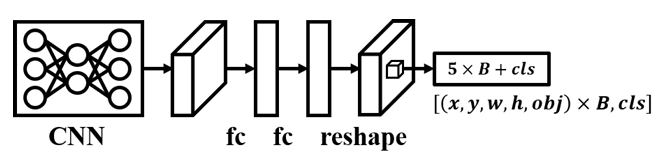
\includegraphics[width=\linewidth]{images/013Methods/yolov1_arch.png}
    \caption{v1}
    \label{subfig_yolov1}
  \end{subfigure}
  \hfill
  \begin{subfigure}{0.32\textwidth}
    \centering
    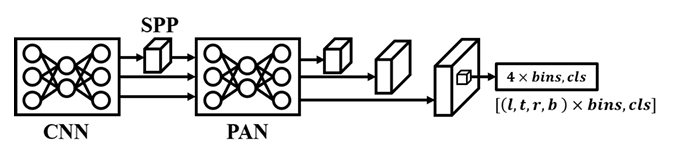
\includegraphics[width=\linewidth]{images/013Methods/yolov8_arch.png}
    \caption{v8}
    \label{subfig_yolov8}
  \end{subfigure}
  \hfill
  \begin{subfigure}{0.32\textwidth}
    \centering
    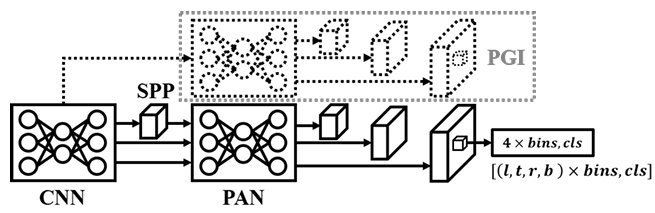
\includegraphics[width=\linewidth]{images/013Methods/yolov9_arch.png}
    \caption{v9}
    \label{subfig_yolov9}
  \end{subfigure}
  
  \caption{Different YOLO Architectures}
\end{figure}



% \begin{itemize}
%     \item Weiterentwicklung von YOLO zeigt sich in dem Unterschied zur Archtektur von YOLOv1 über v8 bis zu v9
%     \item yolov1 kann durch die One Stage Methode eine große Anzahl von Parametern und Berechnungen vermeiden, da Sie durch die   \acrshort{FCL} in der zweiten Schicht erzeugt werden
%     \item yolov8 basiert auf yolov5 und nimmt azhlreiche optimierungen hinzu. Die \acrfull{ELAN} Integration aus YOLOv7 wird um eine zusätzliche Residual Connection erweitert und der Decoder, basierend auf YOLOv6, bleibt identisch
%     \item Yolov8 hat eine Verbesserung der Trainingsleistung von 30\% udn bietet verschiedene Möglichkeiten um nachgelagerte Aufgaben des Downstreamdetectors zu ermöglichen (wie segment anything, instance segmentation, pose estimation, multiple object tracking)
%     \item yolov9 kann durch die \acrshort{PGI} Integartion das Problem vermeiden, dass wichtige Informationen bei der oberflächlichen Netzebene verloren gehen. PGI sorgen für eine robustere Leistung ,weil die Originalinformaitonen maximal tief beibehalten werden
% \end{itemize}

Die Entwicklung von \acrshort{YOLO} über die verschiedenen Versionen hinweg zeigt deutliche Fortschritte. Während \acrshort{YOLO}v1 (s. Fig. \ref{subfig_yolov1}) durch die One-Stage-Methode eine große Anzahl an Parametern und Rechenaufwand einsparen konnte, indem Vorhersagen durch die \acrshort{FCL} in der zweiten Schicht erzeugt wurden, baut \acrshort{YOLO}v8 (s. Fig. \ref{subfig_yolov8}) auf \acrshort{YOLO}v5 auf und integriert zahlreiche Optimierungen \cite{Wang2024_yolo_review}. Dazu gehört die \acrfull{ELAN}-Integration aus \acrshort{YOLO}v7, die um eine zusätzliche Residual Connection erweitert wurde, während der Decoder auf \acrshort{YOLO}v6 basiert und unverändert bleibt. Diese Version zeigt zudem eine Verbesserung der Trainingsleistung um etwa 30\% und ermöglicht verschiedene nachgelagerte Aufgaben wie Segmentierung, Instanzsegmentierung, Posenabschätzung und Multiple-Object-Tracking. \acrshort{YOLO}v9 (s. Fig. \ref{subfig_yolov9}) integriert schließlich \acrshort{PGI}, um zu verhindern, dass wichtige Informationen auf oberflächlicher Netzebene verloren gehen. \acrshort{PGI} sorgen für eine robustere Leistung, indem die Originalinformationen maximal tief beibehalten werden \cite{Wang2024_yolo_review}.


Die zentralen Stärken von \acrshort{YOLO}v9 liegen in seiner hohen Verarbeitungsgeschwindigkeit sowie der präzisen Objekterkennung, wodurch eine effiziente Analyse großer Datensätze ermöglicht wird. 


Die Varianten \acrshort{YOLO}v9u und \acrshort{YOLO}v9e unterscheiden sich primär hinsichtlich des verwendeten Labelformats. \acrshort{YOLO}v9e verwendet ein normiertes Koordinatensystem:
\hypertarget{eq:yolov9}{}
\begin{equation}
x_\text{norm} = \frac{x_\text{pixel}}{w_\text{image}},\;\;
y_\text{norm} = \frac{y_\text{pixel}}{h_\text{image}},\;\;
w_\text{norm} = \frac{w_\text{box}}{w_\text{image}},\;\;
h_\text{norm} = \frac{h_\text{box}}{h_\text{image}}
\end{equation}
\label{Eq:yolov9}

\hypertarget{eq:yolov9u}{}
\acrshort{YOLO}v9u hingegen verwendet ein Polygonformat:
\begin{equation}
(\text{class\_index},\ x_1, y_1, x_2, y_2, x_3, y_3, x_4, y_4).
\end{equation}

%\todo{passt das so rein? überhaupt sinnvoll? verstehen und so...}
% Die YOLOv9-Architektur nutzt einen tiefen, GELAN-basierten Backbone mit umfangreicher Feature-Fusion (\texttt{CBLinear}, \texttt{CBFuse}) und Downsampling-Blöcken (\texttt{ADown}), wodurch klassische achsenausgerichtete Bounding-Boxes über den \texttt{Detect}-Layer erzeugt werden. YOLOv9u hingegen verfolgt einen schlankeren Aufbau mit flacherem Backbone, reduzierter Tiefe der \texttt{RepNCSPELAN4}-Blöcke und minimaler Backbone-Fusion. Die Downsampling-Stufen erfolgen hier über einfache Convolutionen, und die Detektion zielt auf orientierte Bounding-Boxes (\texttt{OBB}) ab. Somit besteht ein klarer Trade-off zwischen Modellkomplexität und Effizienz sowie spezialisierter Detektionsfähigkeit.


% Dieses unterschiedliche Labelformat reflektiert die jeweiligen Stärken der Modelle: \texttt{YOLOv9e} ist auf axis-aligned Bounding Boxes optimiert, während \texttt{YOLOv9u} die präzise Darstellung orientierter Objekte ermöglicht.


% \begin{itemize}
%     \item Beide Varianten \acrshort{YOLO}v9u und \acrshort{YOLO}v9e unterscheiden sich durch das genutzte Labelformat
%     \item yolov9e: normalized_x = x_pixel / image_width normalized_y = y_pixel / image_height  normalized_width = box_width_pixel / image_width  normalized_height = box_height_pixel / image_height
%     \item yolov9u: class_index x1 y1 x2 y2 x3 y3 x4 y4
% \end{itemize}

%\todo{Unterschiedliches Labelformat beider Varianten erklären? und bei Implementierung auf Abschnitt verweisen?}

\subsection{YOLOv9u by Wong Kin Yiu}
\label{subsec:yolov9u}

Die Implementierung von \acrshort{YOLO}v9u basiert auf der Version \acrshort{YOLO}v8.1.23 \cite{yolo_v9u_github}, um die ursprüngliche \acrshort{YOLO}v9 Version um diverse nachgelagerte Aufgaben zu erweitern. Hierzu zählen Instanzsegmentierung, orientierte Objekterkennung, Posenabschätzung, Bildklassifikation sowie transformerbasierte Objekterkennung \cite{wang2024}, wobei mit \acrshort{YOLO}v8 als Basis ein \textit{Detect}-Layer integriert wird, der die Vorhersage orientierter \acrshort{BB} ermöglicht. In der vorliegenden Arbeit wird \acrshort{YOLO}v9u eingesetzt, da diese als Open-Source-Variante verfügbar ist und die zugrundeliegende Methodik durch das veröffentlichte Paper dokumentiert wurde \cite{wang2024_sapkota}. Das Modell \acrshort{YOLO}v9e wird von Ultralytics bereitgestellt, jedoch ohne begleitende wissenschaftliche Veröffentlichung, sodass dessen Aufbau und methodische Grundlagen nicht nachvollziehbar dokumentiert sind \cite{ultralyics_2023}.

 


% Die Implementierung von \texttt{YOLOv9u} basiert auf der Version \texttt{YOLOv8.1.23}\cite{yolo_v9u_github} und stellt eine umfassende Weiterentwicklung der \acrshort{YOLO}-Architektur im Vergleich zu \acrshort{YOLO}v8 durch den Einsatz von \acrshort{PGI} und \acrshort{GELAN} dar. Der Einsatz von \acrshort{PGI} ermöglicht die vereinfachte Anwenung neuer leichtgewichtiger Netzwerkarchitekturen und löst das Problem der Verwendung von Deep Supervision nur für extrem tiefe neuronale Netze. Das Nutzen von des von \citeauthor{wang2024_sapkota} entworfenen \acrshort{GELAN} kann durch die Verwendung der herkömmlichen Faltungen eine höhere Parameterauslastung erreichen. Dies bietet auc hVorteile für die Geschwindigkeit und Genauigkeit. Neben der klassischen Objekterkennung unterstützt \texttt{YOLOv9u} durch die Basis von \acrshort{YOLO}v8 zusätzliche Aufgaben wie Instanzsegmentierung, orientierte Objekterkennung, Posenabschätzung, Bildklassifikation sowie transformerbasierte Objekterkennung\cite{wang2024}. Damit bietet das Modell eine erweiterte Funktionalität gegenüber früheren \acrshort{YOLO}-Versionen, sowie der originalen \acrshort{YOLO}v9-Version, und eignet sich insbesondere für komplexe Szenarien mit mehreren Aufgabenstellungen innerhalb eines Frameworks. Diese Version wird genutzt, da sie \acrlong{obb} unterstützt.

\subsection{YOLOv9e by Ultralytics}
\label{subsec:yolov9e}

Die \acrshort{YOLO}v9-Modellreihe von Ultralytics umfasst mehrere Varianten, die sich in Bezug auf Modellgröße, Genauigkeit und Rechenkomplexität unterscheiden. Alle Varianten integrieren die von \citeauthor{wang2024_sapkota} entwickelten \acrshort{PGI}- und \acrshort{GELAN}-Architekturen und unterstützen zudem die Verarbeitung von \acrshort{abb}. Die Bandbreite reicht von der kompakten \texttt{YOLOv9t}-Variante mit einer Eingabebildgröße von $640 \times 640$ Pixeln, 2 Millionen Parametern und 7{,}7 \acrshortpl{GFLOP} bis hin zur leistungsstärksten \acrshort{YOLO}v9e-Variante mit 58{,}1 Millionen Parametern und 192{,}5 \acrshortpl{GFLOP} (siehe Tabelle~\ref{tab:yolov9-models}).  

Aufgrund der höchsten erzielten Genauigkeit (\acrshort{mAP}50-95 = 55,6) sowie der höchsten Rechenkapazität wurde das \texttt{YOLOv9e}-Modell für alle Experimente mit axis-aligned Bounding Boxes verwendet. Die Wahl dieser Variante erfolgte mit dem Ziel, die maximale Detektionsleistung im Rahmen der Evaluierung sicherzustellen. Zudem wird diese Version genutzt, da sie die Verarbeitung von \acrlong{abb} unterstützt.

% \subsection{Differences YOLOv9u and YOLOv9e}
% \todo{wirklich nötig?}
% Die YOLOv9-Architektur und ihre Variante YOLOv9u unterscheiden sich in mehreren wesentlichen Aspekten, die sowohl die Modellkomplexität als auch die Detektionsfähigkeiten betreffen. YOLOv9 verwendet einen tiefen, GELAN-basierten Backbone, der mehrere Feature-Fusionsblöcke (\texttt{CBLinear}, \texttt{CBFuse}) sowie Downsampling-Blöcke (\texttt{ADown}) integriert. Diese Struktur ermöglicht eine intensive Mischung von Merkmalen über unterschiedliche Auflösungsebenen hinweg und unterstützt dadurch die Erkennung von Objekten in verschiedenen Skalen. Der Head von YOLOv9 kombiniert Features auf mehreren Ebenen mittels Upsampling und Concat-Operationen und erzeugt klassische, achsenausgerichtete Bounding-Boxes über den finalen \texttt{Detect}-Layer.  

% Im Gegensatz dazu verfolgt YOLOv9u einen kompakteren und effizienteren Aufbau. Der Backbone ist flacher und verzichtet weitgehend auf interne Feature-Fusionen im Vergleich zu YOLOv9. Downsampling erfolgt hier über einfache Convolutional-Blöcke mit Stride 2, und die Tiefe der \texttt{RepNCSPELAN4}-Blöcke ist reduziert. Im Head werden die Features ebenfalls mittels Upsampling und Concat kombiniert, jedoch ohne die zusätzlichen Downsampling-Blöcke des Originals. Ein entscheidender funktionaler Unterschied besteht darin, dass YOLOv9u orientierte Bounding-Boxes (\texttt{OBB}) generiert, während YOLOv9 klassische Bounding-Boxes liefert.  

% Zusammenfassend lässt sich sagen, dass YOLOv9 eine komplexere und tiefere Architektur mit intensiver Feature-Fusion darstellt, die tendenziell eine höhere Genauigkeit bei klassischen Bounding-Boxes ermöglicht. YOLOv9u hingegen bietet eine schlankere, effizientere Struktur mit reduzierter Rechenlast und ist speziell für die Detektion orientierter Objekte optimiert. Die Wahl zwischen beiden Varianten hängt somit von den Anforderungen an Genauigkeit, Rechenaufwand und Art der zu detektierenden Objekte ab.


\begin{table}[h]
\centering
\begin{tabular}{l|c|c|c|c|c} % keine äußeren vertikalen Linien
\textbf{Model} & \textbf{Image Size} & \textbf{mAP$_{\text{val}}$ 50--95} & \textbf{mAP$_{\text{val}}$ 50} & \textbf{Parameters (M)} & \textbf{FLOPs (B)} \\
\hline
YOLOv9t & 640 & 38.3 & 53.1 & 2.0 & 7.7 \\
YOLOv9s & 640 & 46.8 & 63.4 & 7.2 & 26.7 \\
YOLOv9m & 640 & 51.4 & 68.1 & 20.1 & 76.8 \\
YOLOv9c & 640 & 53.0 & 70.2 & 25.5 & 102.8 \\
YOLOv9e & 640 & 55.6 & 72.8 & 58.1 & 192.5 \\
\end{tabular}
\caption{Comparison of YOLOv9 model variants in terms of accuracy and computational complexity at an input resolution of 640$\times$640 pixels. \cite{ultralyics_yolov9,wang2024_sapkota}}
\label{tab:yolov9-models}
\end{table}



%##########################################################################
%##########################################################################
%##########################################################################
%##########################################################################
%##########################################################################
%##########################################################################
%##########################################################################
%##########################################################################


\section{Programming Environment}
Die genutzte Programmiersprache ist Python. Die Scripte für den \acrshort{HPC} \acrshort{PALMA} wurden in Bash geschrieben.

\subsection{Python Packages}
Es wurden diverse Python Packages zur Implementierung genutzt, die im folgenden kurz beschrieben werden. 
\subsubsection{Computer Vision 2}
Ein Teil der "Open Source Computer Vision" Bibliothek ist \Acrfull{CV2} \cite{opencv_about}. Die aktuelle Version 4.12.0 wurde am 09.07.2025 veröffentlicht \cite{opencv_release}. \\
Die Bibliothek bietet Algorithmen und Funktionen zur Bild- und Videobearbeitung an, die in dieser Arbeit hauptsächlich dazu genutzt werden, die verschiedenen Kanäle zu neuen Bildern zu kombinieren. Hierbei ist zu beachten, dass \acrshort{CV2} Bilder als BGR (Blue, Green, Red) Farbkombination abspeichert, was zu Falschfarbdarstellungen einiger Abbildungen, die in RGB abgeildet werden, (wie Fig. \ref{fig:perm_exp_example_pics}) führen kann.
\subsubsection{Numpy}
Ein weiteres Open-Source Projekt ist NumPy, welches 2005 gegründet wurde, um numerische Operationen in Python zu implementieren \cite{numpy_about}. Die aktuelle Version ist 2.3.0 und wurde am 07.06.2025 veröffentlicht \cite{numpy_main_web}. \\
Mithilfe dieser Bibliothek kann eine zufällige Verteilung der Bilddaten auf die Folds realisiert werden, indem die eingelesene Bildliste einer zufälligen Permutation unterzogen wird. Darüber hinaus stellt die Bibliothek Funktionen zur Verfügung, mit denen sowohl die Berechnung und Reskalierung des \acrshort{NDVI}-Kanals als auch die Transformation der Bounding-Box-Koordinaten in das für das \acrshort{YOLO}-Framework erforderliche Format durchgeführt werden können. Zusätzlich ermöglicht sie die Umrechnung axis-aligned Bounding Boxes in oriented Bounding Boxes sowie die Flächenberechnung beider Bounding-Box-Typen.
\subsubsection{Scipy}
SciPy ist in der Version 1.16.0 am 22.06.25 veröffentlicht worden \cite{scipy-main}. Diese Bibliothek bietet Algorithmen für wissenschaftliche Berechnungen in Python an \cite{scipy-main}. Die Unterfunktion "ConvexHull" wird zur Flächenberechnung der oriented Bounding Boxen genutzt.
\subsection{Additional Python-Packages for data analysis}
Zur Analyse der Modelle wurden die folgenden Bibliotheken verwendet.
\subsubsection*{Matplotlib}
Die Bibliothek "Matplotlib" wurde in der Version 3.10.0 am 23.12.2024 veröffentlicht\cite{matplotlib}. Im Rahmen dieser Arbeit werden durch diese Erweiterung die Datenanalysen und die Ausgabe der Plots ermöglicht.
\subsubsection*{Seaborn}
"Searborn" ist in der Version 0.13.2 im Januar 2024 veröffentlicht worden \cite{seaborn}. Die Bibliothek ermöglicht das Erstellen von Grafiken, wie Boxplots, zur vereinfachten Datenanalyse.
\subsubsection*{pandas}
Die Bibliothek "pandas" ist ebenfalls ein Open Source Datenanalyse und -manipulierungstool. Die aktuelle Version 2.3.1 wurde am 07.07.2025 veröffentlicht. Die Bibliothek wird auch zur Datenanalyse in dieser Arbeit verwendet \cite{pandas}.

%!TEX root = ../thesis.tex
\chapter{Implementation}
\label{ch:implementation}




\section{Challenges Preprocessing}
Bei der Verarbeitung des VEDAI-Datensatzes traten mehrere technische Herausforderungen auf. 
Zunächst mussten die vorhandenen Label in das \acrshort{YOLO}v9-\acrshort{obb}-Format konvertiert werden, um mit dem gewählten Modell kompatibel zu sein. 
Dabei zeigte sich, dass ein kleiner Teil der Daten (7 von 3\,757 Instanzen) Koordinatenwerte aufwies, die außerhalb des zulässigen Bereichs lagen (d.\,h. kleiner als 0 (s. Fig. \ref{fig:smaller0}) oder größer als 1 (s. Fig. \ref{fig:higher1})) . 
Dieses Problem wurde durch den Einsatz von Exception Handling sowie durch Rundung der Werte auf den gültigen Wertebereich behoben. 

\begin{figure}[h]
    \centering
    \begin{subfigure}[b]{0.45\textwidth}
        \centering
        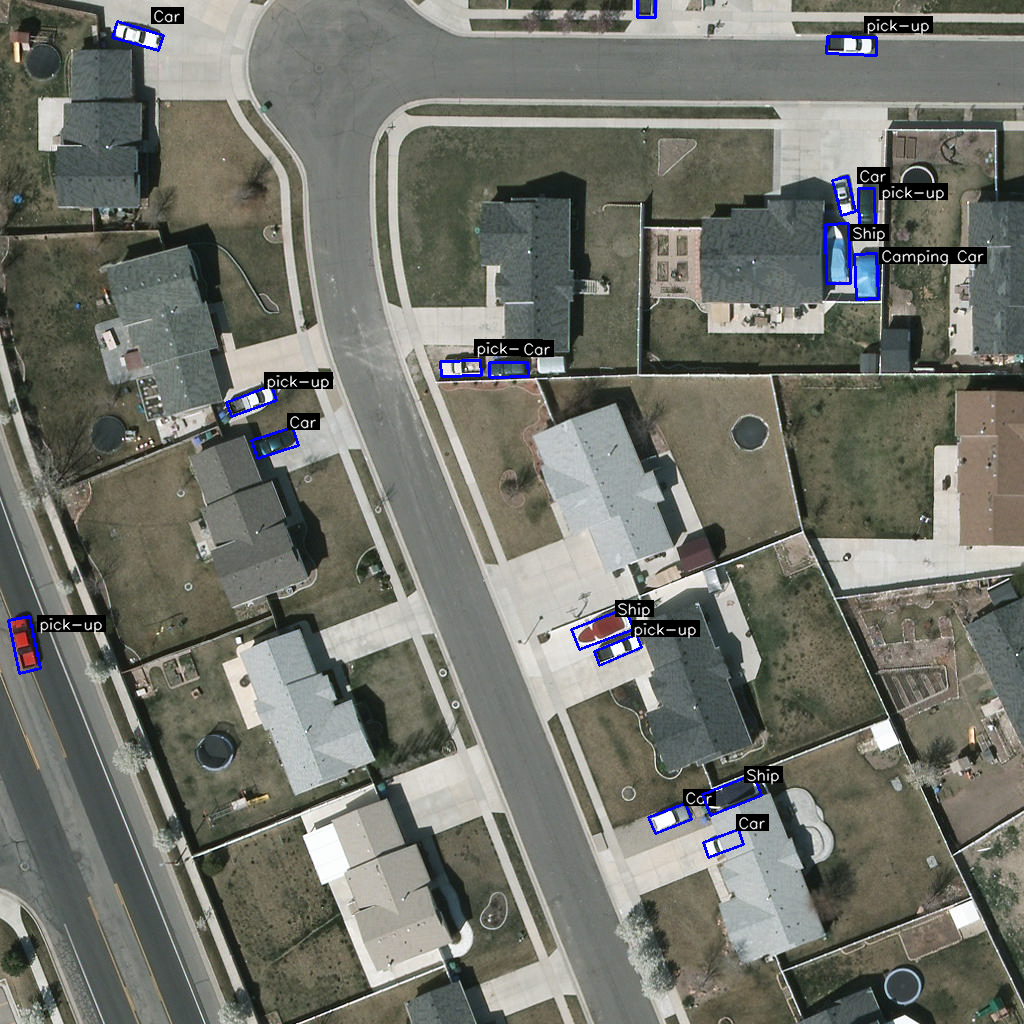
\includegraphics[trim={600pt 1000pt 350pt 0pt},clip,width=\textwidth]{images/bb_smaller0.png}
        \caption{Two Coordinate out of range and smaller 0}
        \label{fig:smaller0}
    \end{subfigure}
    \hfill
    \begin{subfigure}[b]{0.45\textwidth}
        \centering
        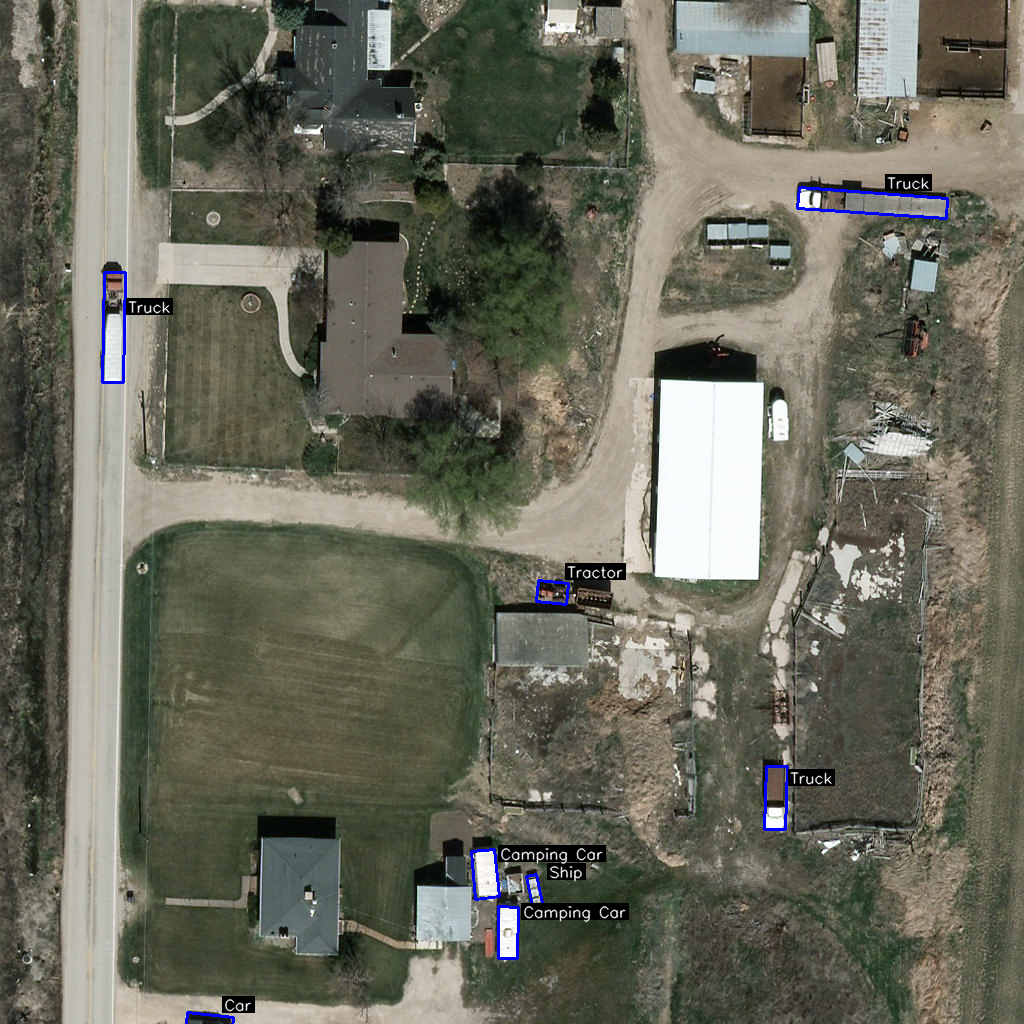
\includegraphics[trim={180pt 0pt 750pt 993pt},clip,width=\textwidth]{images/bb_higher1.png}
        \caption{Two Coordinates out ouf range and higher 1}
        \label{fig:higher1}
    \end{subfigure}
    \caption[Example for label coordinates outside of the image]{Example for label coordinates outside of the image (for full-sized Image see \ref{fig:example_coords_ooR_fs})}
    \label{fig:example_coords_ooR}
\end{figure}

% Da die von \citeauthor{Razakarivony2015} \cite{Razakarivony2015} verwendeten Folds nicht disjunkt waren, erhöhte sich das Risiko von Overfitting (s. Kap. \ref{subsec:overfitting}), sodass eigene Folds erstellt werden mussten (s. Kap. \ref{subsec:Fold_creation}), deren Verteilung im folgenden Abschnitt beschrieben wird. \todo{satz überarbeitne, doppelung}






\section{6-Fold-Cross-Validation}
\label{sec_5Fold_CV}

Um die Robustheit der Ergebnisse sicherzustellen und eine fundierte Vergleichbarkeit verschiedener Modelle zu ermöglichen, wurde in dieser Arbeit eine 6-Fold-Cross-Validation angewendet. Insbesondere wurde Wert darauf gelegt, die Evaluation nicht nur auf einem Teildatensatz durchzuführen, sondern eine Mehrfachteilung der Daten vorzunehmen, sodass Schwankungen durch unterschiedliche Trainings- und Validierungsaufteilungen minimiert werden.

Im Gegensatz zu den von \citeauthor{Razakarivony2015} \cite{Razakarivony2015} bereitgestellten Folds, deren Zusammenstellung identische Bilder gleichzeitig im Trainings- und Validierungssatz aufweist, wurden für diese Arbeit eigene, disjunkte Folds generiert. Letztere gewährleisten, dass keine Überlappungen zwischen Trainings- und Validierungsdaten existieren und somit die Gefahr von verfälschten Trainingsergebnissen durch Overfitting ausgeschlossen ist. Die genaue Methodik der Fold-Erstellung ist in Kapitel \ref{subsec:Fold_creation} beschrieben. 

Die Datenaufteilung erfolgte in sechs Folds (0-5): Fünf Folds (Fold 0 bis 4) wurden jeweils für Training und Validierung genutzt, während Fold 5 ausschließlich für abschließende Testzwecke reserviert blieb. Dadurch wurde erreicht, dass die finale Evaluation auf bisher ungesehenen, neutralen Daten stattfand.

Ein besonderes Augenmerk galt einer homogenen Verteilung der Objekte und Objektklassen über alle Folds hinweg. Jeder Fold umfasst zwischen 207 und 221 Bilder, darin enthalten sind jeweils drei bis sieben reine Hintergrundbilder ohne Objekte. Dies ermöglichte eine ausgewogene und repräsentative Bewertung der Modelle hinsichtlich aller vorkommenden Klassen. Die resultierende Klassen- und Bildverteilung pro Fold ist in Tabelle~\ref{tab:fold_distribution} dargestellt.

Insgesamt trägt dieses Verfahren dazu bei, dass die experimentellen Resultate eine hohe Validität aufweisen und zuverlässig Rückschlüsse auf die Auswirkungen der zusätzlichen Kanäle bei den verwendeten Modelle erlauben.


\begin{table}[h!]
\centering
\begin{tabular}{lcccccc}
\textbf{Class/Fold} & \textit{0} & \textit{1} & \textit{2} & \textit{3} & \textit{4} & \textit{5} \\
\hline
\textit{Car}              & 229 & 239 & 226 & 225 & 240 & 225 \\
\textit{Truck}            & 51  & 57  & 50  & 49  & 51  & 50  \\
\textit{Ship}             & 30  & 28  & 29  & 30  & 27  & 27  \\
\textit{Tractor}          & 30  & 32  & 33  & 30  & 31  & 30  \\
\textit{Camping car}      & 65  & 72  & 64  & 69  & 64  & 63  \\
\textit{Van}              & 18  & 17  & 17  & 17  & 16  & 16  \\
\textit{Vehicle}          & 34  & 37  & 34  & 34  & 39  & 33  \\
\textit{Pick-Up}          & 164 & 161 & 157 & 160 & 159 & 157 \\
\textit{Plane}            & 4   & 11  & 4   & 18  & 4   & 7   \\
\textit{Quantity Images}  & 206 & 214 & 221 & 211 & 207 & 209 \\
\textit{Background Images}& 7   & 3   & 3   & 3   & 3   & 3   \\
\hline
\end{tabular}
\caption{Class distribution across folds.}
\label{tab:fold_distribution}
\end{table}
% \begin{itemize}
%         \item Cross validation to ensure robustness and better comparison of different models
%         \item create own folds, as the ones provided by the paper had the same images in training and validation data
%         \item  6 Folds
%         \item 5 for Training and Validation, 1 for Test (Fold 5)
%         \item Good object distribution between the folds
%         \item 207-221 Images per Fold, where 3 or 7 Images are only background
        
%         \item Methodik wurde in Sec. \ref{subsec:Fold_creation} beschrieben
%         \item \todo{Tabelle mit Verteilung einfügen}
%         \item Sagen das die ursprünglichen Fodls des VEDAI Datasets nicht disjunkt sind -> Trainingsergebnisse verfälscht, deshalb eigene Folds erstellt
%     \end{itemize}


% \subsection{YOLOv9u}
% \begin{itemize}
%     \item Implementierung von YOLOv9 auf Basis von YOLOv8.1.23 \cite{yolo_v9u_github}
%     \item erweiterung von yolov9 mit object detection, instance segmentation, oriented object detection, pose estimation, image classficitation, transformer-based object detection \cite{wang2024yolov9}
% \end{itemize}
% \subsection{YOLOv9e}
% \begin{itemize}
%     \item yolov9 Modelle reichen von der t variante mit (imgsize: 640, flops 7.7) bis zur e variante mit (192,5 gflops)
%     \item aufgrund der besten genauigketi und der höchsten flop rate wird das yolov9e modell bei den axis aligend bounding boxen genutzt
% \end{itemize}
% \subsection{Hyperparameter}
% \todo{wird bei Implementierung beschrieben, hier raus nehmen?}


% \begin{itemize}
%     \item DOTA bietet sich als pretrained Model Datengrundlage für die Permutationsexperimente an, da es viele verschieden Klassen auf Satellitenbildern enthält
%     \item Bildgröße von 800 \texttimes 800 bis 20.000 \texttimes 20.000 Pixel
%     \item 3 Channel (Red, Green, Blue) und Grayscale Images (Panchromatic Band von GF2 und JL1 Satelliten)
%     \item Satellite Images von Google Earth und anderne Quellen
%     \item \todo{Bsp. Bild für jede Klasse zeigen (aus Paper nehmen!; Quellenverlinkung für text und bild nicht vergessen); habe alle 16 Klassen für das Training genutzt, wichtig sind trotzdem nur Large Vehicle, Plane, Ship, small vehicle}
% \end{itemize}


\section{High-Performance-Cluster PALMA}

Für das Training der Modelle wurde das \acrfull{HPC} \Acrshort{PALMA} der Universität Münster genutzt. Als Arbeitsumgebung kam dabei eine isolierte \texttt{Python}-Umgebung (UV \cite{palma_uv}) zum Einsatz. Die Ausführung der Trainingsprozesse erfolgte über selbst entwickelte \texttt{Bash}-Skripte, die auf unterschiedlichen \acrshort{GPU}-Knoten des Clusters (u.\,a. HGX-Knoten) verteilt wurden, um eine effiziente Parallelisierung der Trainings zu ermöglichen.

PALMA (Abkürzung für "\Acrlong{PALMA}") wird von dem \Acrfull{CIT} der Universität Münster, basierend auf Hardware der Firma MEGWARE, bereitgestellt \cite{palma_spec} und verfügt über die in Tab. \ref{tab:Spec_Palma} technische Spezifikationen \cite{palma_spec}:



\begin{table}[h!]
\centering
\begin{tabular}{ll}
\multicolumn{2}{c}{\textbf{Palma Specifications}} \\ \hline
\textbf{Total number of \acrshort{CPU} cores} & 16,272 \\
\textbf{Memory} & 77,568\,\acrshort{GB} \\
\textbf{Number of compute nodes} & 444 \\
\textbf{Processor} & Intel Xeon Gold 6140 (18~cores, 2.30\,\acrshort{GHz}, Skylake architecture) \\
\textbf{Network interconnect} & 100\,\acrshort{GHz}/s Intel Omni-Path \\
\textbf{Storage system} & \acrshort{GPFS} with a total capacity of 2.4\,\acrshort{PB} \\
\textbf{Linpack performance} & \textit{R\textsubscript{max}} = 800\,\acrshort{TFLOP}/s; \textit{R\textsubscript{peak}} = 1,277\,\acrshort{TFLOP}/s \\
\textbf{Operating system} & Rocky Linux 9 \\
\hline
\end{tabular}
\caption{System overview PALMA}
\label{tab:Spec_Palma}
\end{table}

Die hohe Rechenleistung und Speicherkapazität des Clusters machten es möglich, auch komplexe Trainingsprozesse mit vielen hochauflösenden Bilddaten effizient und schnell zu verarbeiten.
% \begin{itemize}
%     \item UV als Python Umgebung auf Palma genutzt
%     \item Bash Scripte geschrieben um die Modelle auf diversen GPUS (HGX, etc) zu trainieren
% \end{itemize}
% \begin{itemize}
%     \item Hersteller: MEGWARE\cite{palma_spec}
%     \item 16.272 Cores
%     \item 77.568 GB Memory
%     \item 444 Nodes
%     \item Processor: Intel Xeon Gold 6140 18C @ 2.30GHz (Skylake)
%     \item Interconnect 100Gbit/s Intel Omni-Path
%     \item GPFS Storage: 2,4 PB
%     \item Linpack Performance: Rmax: 800 TFlop/sRpeak: 1,277 TFlop/s
%     \item OS: Rocky Linux 9 
% \end{itemize}

% \subsection{Challenges Preprocessing}
% \subsubsection{VEDAI Dataset Challenges}
% \begin{itemize}
%     \item Label müssen in yolov9 obb format konvertiert werden
%     \item kleine Anzahl (7/3757) war kleiner als 0 oder größer als 1
%     \item Lösung mit Exception Handling und Runden der Werte
%     \item \todo{Beispielbilder einfügen}
% \end{itemize}

% \section{Workflow}
% \subsection{Axis Aligned vs. Oriented Bounding Boxes}
% \begin{itemize}
%     \item Vergleich zwischen Axis Aligned udn Oriented Bounding Boxen
%     \item YOLOv9 arbeitet ursprünglich nur mit aab Boxen
%     \item YOLOv9u kann mit obb arbeiten, da Codebasis von YOLOv8 von Ultralytics, was obb unterstützt
%     \item 
% \end{itemize}
% \begin{itemize}
%     \item \todo{Vergleichsbilder (Schiff und Auto Vergleich) einfügen}
%     \item mehr Blankspace bei axis aligned Bbs
%     \item Concentration of the box on the actual object, significantly less surrounding area outlined. No overlap between bounding boxes (Bei Ship bb)
%     \item 
% \end{itemize}
% \subsection{Channel Permutation}
% \begin{itemize}
%     \item Folgende Permutation werden im Rahmen der Arbeit evaluiert: RGBIR, IRGB, RIRB; RGB, RGIR, RGBNDVI, GBNDBVI
% \end{itemize}
% \subsection{DOTA Training}
% \begin{itemize}
%     \item DOTA als Pretrained Modell für Channel Permutation, map50-95 around 0.4 and training over around 800 epcohs 
%     \item \todo{Result.png einfügen? oder doch sein lassen?}
% \end{itemize}
% \subsection{Ablation Studie}
% \begin{itemize}
%     \item Ablation Study für R, G, B, IR, NDVI durchgeführt
% \end{itemize}


\section{Bash Scripts}

Für das Training der Modelle wurden mehrere \texttt{Bash}-Skripte entwickelt, die für den Hochleistungsrechner \acrshort{PALMA} ausgelegt waren. Die Trainingsläufe erfolgten primär über \acrshort{SLURM} Job Arrays, wobei jeder Fold einer Permutation einem separaten Job zugeordnet wurde. Somit entsprach ein Modell stets einem Fold innerhalb einer bestimmten Permutation.  

Die Entscheidung zwischen \acrlong{abb} und \acrlong{obb} erfolgte unter denselben Trainingsparametern wie bei den Permutationsexperimenten (s. Tab.~\ref{tab:hyperparameters}), jedoch mit unterschiedlichen Modellen: \acrshort{YOLO}v9e für \acrshort{abb} und \acrshort{YOLO}v9u für \acrshort{obb}, da jeweils nur diese Varianten die entsprechenden Bounding-Box-Formate unterstützen. In diesem Fall wurde kein vortrainiertes Modell genutzt, sondern ein Training \textit{from scratch} durchgeführt.  

Im Anschluss wurden die Permutationsexperimente durchgeführt. Dabei kamen einheitlich die in Tab.~\ref{tab:hyperparameters} aufgeführten Hyperparameter zum Einsatz. Die Bildauflösung betrug 1024~$\times$~1024 Pixel, die Trainingsdauer umfasste 500 Epochen, und ein frühzeitiges Beenden war durch einen \texttt{patience}-Wert von 0 deaktiviert, um eine konsistente Vergleichbarkeit sicherzustellen. Grundlage war ein auf dem \acrshort{DOTA}-Datensatz vortrainiertes Modell, wobei durchgängig die Architektur \acrshort{YOLO}v9u (s. Kap.~\ref{subsec:yolov9u}) verwendet wurde.  

Für die Ablationsstudien wurde hingegen auf den Einsatz eines vortrainierten Modells verzichtet, während alle übrigen Trainingsparameter unverändert blieben.  

Nach Abschluss des Trainings wurde jeweils das Modell mit der besten Validierungsleistung ausgewählt und anschließend auf den entsprechenden Testfold angewendet. Die Evaluation erfolgte in beiden Fällen in einem einmaligen Durchlauf, um konsistente und vergleichbare Ergebnisse zu gewährleisten.  


% Für das Training der Modelle wurden mehrere \texttt{Bash}-Skripte entwickelt, die für den Einsatz auf dem Hochleistungsrechner \acrshort{PALMA} konzipiert wurden. Die Trainingsläufe wurden primär mittels \texttt{\acrshort{SLURM} Job Arrays} durchgeführt, wobei jeder Fold einer Permutation einem eigenen Job zugewiesen wurde. Somit entsprach ein Modell jeweils einem Fold innerhalb einer bestimmten Permutation.

% Für die Entscheidung zwischen \Acrlong{abb} und \Acrlong{obb} wurden die gleichen Trainingsparameter wie bei den Permutationsexperimenten (s. Tab. \ref{tab:hyperparameters}), aber verschiedene Modelle genutzt. YOLOv9e wurde für die \acrshort{abb} Boxen genutzt und YOLOv9u für die \acrshort{obb} Boxen eingesetzt, da nur jeweils diese Modelle die verschiedenen Bounding Box Arten unterstützen. Es wurde kein vortrainiertes Modell verwendet, sondern von Scratch trainiert.

% Im Rahmen des Permutationstrainings kamen für sämtliche Permutationen einheitlich die in Tabelle \ref{tab:hyperparameters} aufgeführten Hyperparameter zum Einsatz. 
% Die Bildauflösung betrug 1024~$\times$~1024 Pixel, die Trainingsdauer umfasste 500 Epochen, und das frühzeitige Beenden des Trainings war durch einen \texttt{patience}-Wert von 0 deaktiviert, um eine konsistente Vergleichbarkeit zu gewährleisten. 

% Verwendet wurde ein vortrainiertes Modell auf dem \acrshort{DOTA}-Datensatz (s. Chap. \ref{subsec:DOTA}), wobei die Modellarchitektur \texttt{YOLOv9u} (s. Chap. \ref{subsec:yolov9u}) durchgängig zum Einsatz kam.

% Für die Ablationsstudien wurde auf den Einsatz des vortrainierten Modelles verzichtet; alle übrigen Trainingsparameter blieben unverändert.

% Nach Abschluss des Trainings wurde jeweils das Modell mit der besten Leistung auf den Validierungsdaten evaluiert. Anschließend erfolgte die Anwendung dieses Modells auf dem entsprechenden Testfold. In beiden Fällen wurde die Evaluation in einem einmaligen Durchlauf durchgeführt, um konsistente und vergleichbare Ergebnisse zu gewährleisten.

\begin{table}[htbp]
\centering

\begin{tabular}{ll}
\hline
\textbf{Hyperparameter} & \textbf{Value / Description} \\
\hline
Task & Oriented Bounding Box (OBB) \\
Mode & Training \\
Model & YOLOv9u, pretrained on \acrshort{DOTA} \\
Dataset & \acrshort{VEDAI}  \\
Epochs & 500 \\
Batch size & 4 \\
Image size & 1024 × 1024 px \\
Early stopping (patience) & 0 (disabled) \\
Optimizer & Auto \\
Initial learning rate ($lr_0$) & 0.01 \\
Momentum & 0.937 \\
Weight decay & 0.0005 \\
Warmup epochs & 3 \\
Data augmentation & FlipLR 0.5, Mosaic 1.0, Erasing 0.4, AutoAugment randaugment \\
Device & GPUs 0,1,2,3 \\
Workers & 8 \\
Save directory & \texttt{/scratch/tmp/t\_liet02/cross\_validation/rgb/fold4} \\
\hline
\end{tabular}
\caption{Key training hyperparameters at the \acrshort{RGB} Permutation (Fold 4)}
\label{tab:hyperparameters}
\end{table}

% \begin{itemize}
%     \item Diverse Bash Scripte für PALMA geschriebne um die Modelle zu trainieren. 
%     \item Hauptsächlich SLURM Job Arrays genutzt um jeweils alle Folds einer Permutation durchlaufen (jeder Fold einer Permutation bekommt einen Job = ein modell)
%     \item hyperparameter (für permutation training): imagesize:1024; epochs: 500, patience: 0 (ausgestellt um zur besseren Vergleichbarkeit alle Modelle immer exakt 500 epochs durchzutrainieren); pretrained true (dota dataset,  ref zu beschreibung einfügen); als modell immer yolov9u (ref einfügen)
%     \item für ablation training: kein pretrained model, sonst alles gleich
%     \item danach immer validierung des besten val modells auf den val daten 
%     \item dann das beste validierungsmodell auf dem testfold
%     \item beides mal nur ein durchlauf daten zur evaluation zu erhalten
% \end{itemize}



\cleardoubleoddemptypage

% %!TEX root = ../thesis.tex
\chapter{Implementation}
\label{ch:implementation}


% \cleardoubleoddemptypage

%!TEX root = ../thesis.tex
\chapter{Results}
\label{ch:results}
This chapter is based on Figure~\ref{fig:Flowchart} and first discusses the comparison of \acrshort{abb} and \acrshort{obb} formats, then the permutation experiments to test robustness, and finally the ablation study to evaluate individual components.

In the image collages (see Fig. \ref{fig:aab_obb_example_pics}, \ref{fig:perm_exp_example_pics} and \ref{fig:ablation_example_pics}) use the colour scheme defined in Table \ref{tab:class_colors} to make the model predictions clearly distinguishable and to ensure unambiguous assignment to the respective classes.

\section{Oriented Bounding Boxes and Axis-aligned Bounding Boxes}
\todo{Bilder in Originalgröße in Appendix packen}
\begin{figure}[h]
    \centering
    
    % Erste Zeile
    \begin{subfigure}[b]{0.45\textwidth}
        \centering
        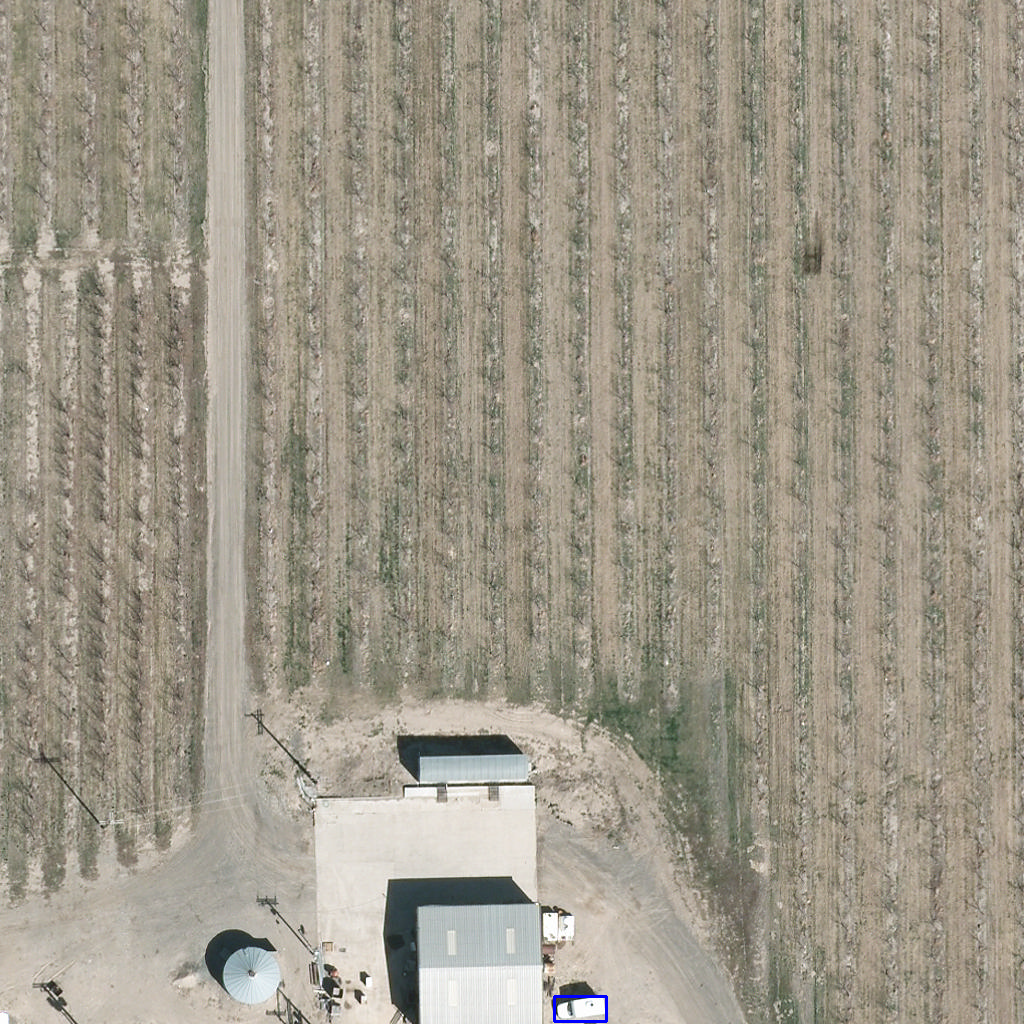
\includegraphics[trim={550pt 0pt 410pt 990pt},clip,width=\textwidth]{images/015Results/01abb_vs_obb/abb_truck.png}
        \caption{Label: "Truck", ABB format, area: $\approx 1378 \text{px}$}
        \label{fig:abb_truck}
    \end{subfigure}
    \hfill
    \begin{subfigure}[b]{0.45\textwidth}
        \centering
        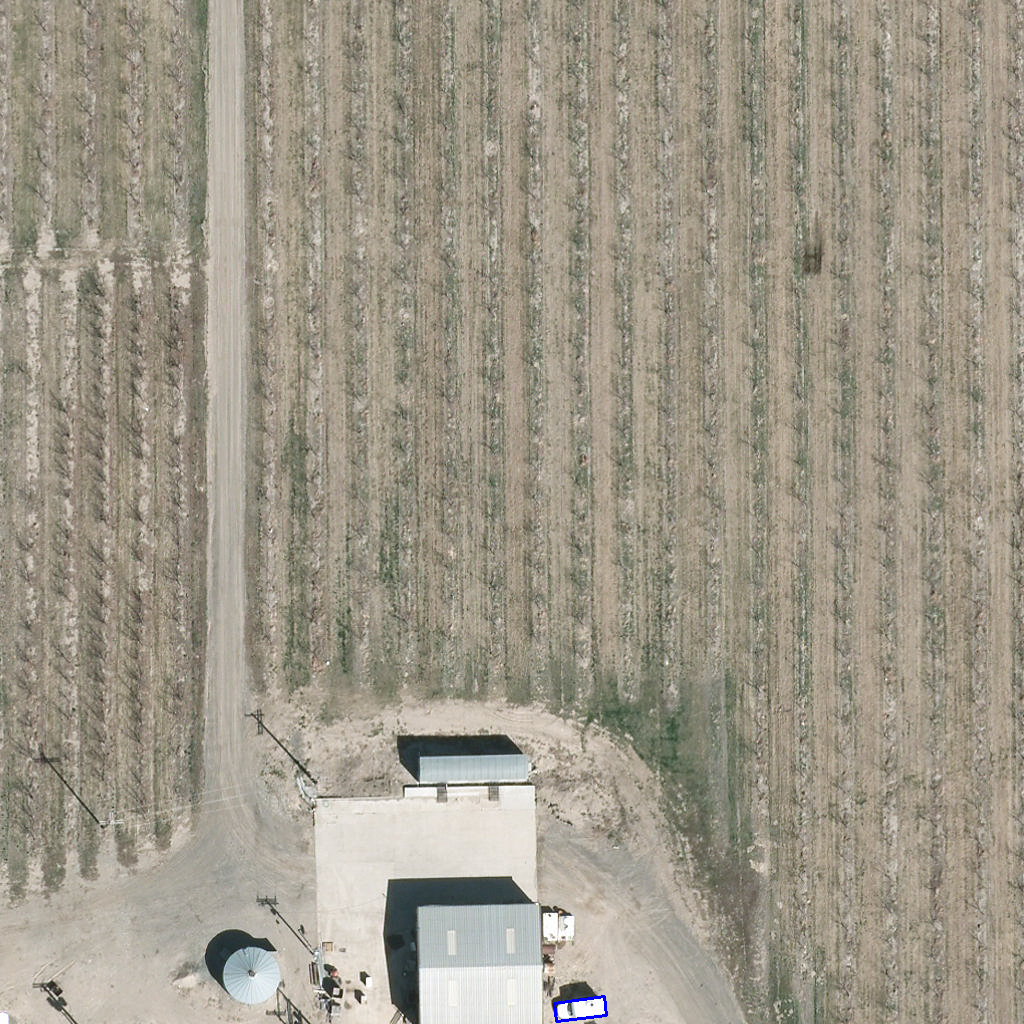
\includegraphics[trim={550pt 0pt 410pt 990pt},clip,width=\textwidth]{images/015Results/01abb_vs_obb/obb_truck.png}
        \caption{Label: "Truck", OBB format, area: $\approx 967 \text{px}$}
        \label{fig:obb_truck}
    \end{subfigure}
    
    \vspace{0.5cm} % Abstand zwischen den Zeilen
    
    % Zweite Zeile
    \begin{subfigure}[b]{0.45\textwidth}
        \centering
        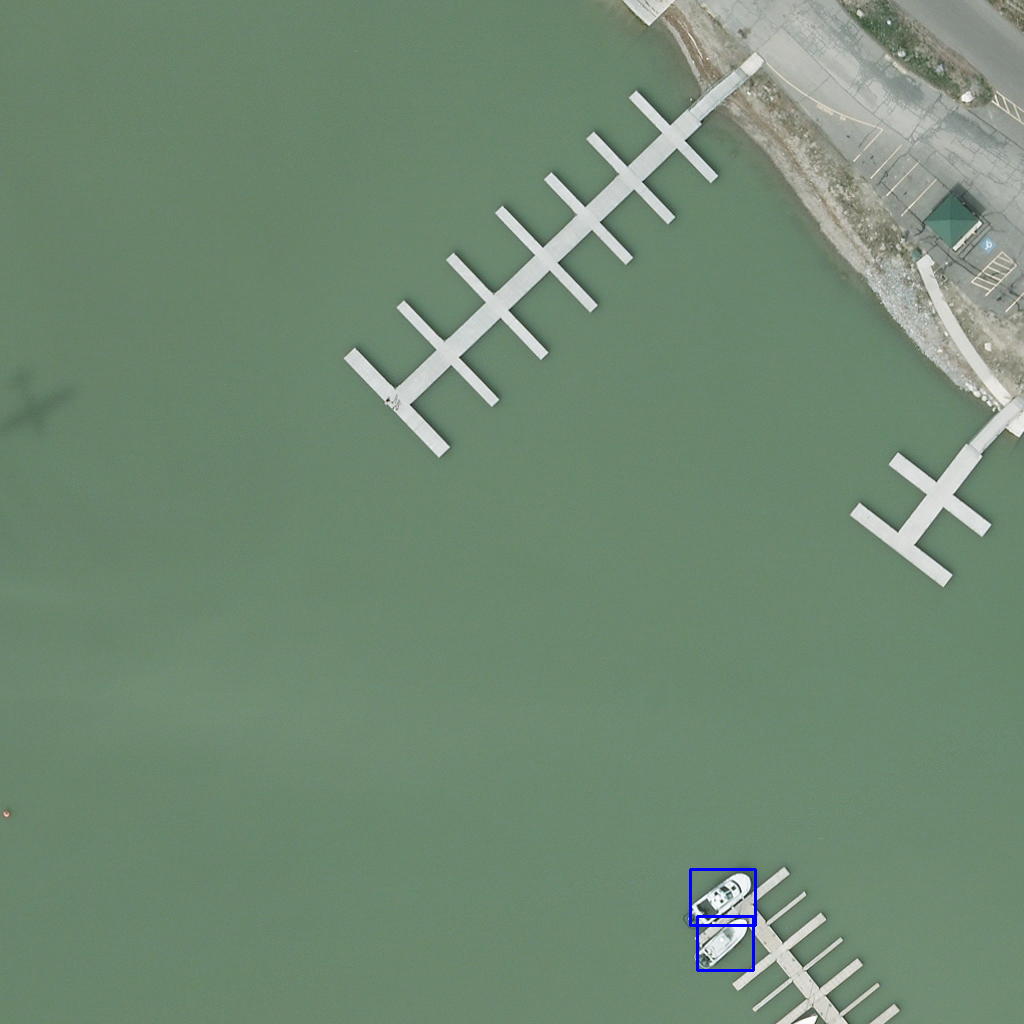
\includegraphics[trim={680pt 50pt 250pt 865pt},clip,width=\textwidth]{images/015Results/01abb_vs_obb/abb_ship.png}
        \caption{Labels: "Ship", ABB format}
        \label{fig:abb_ship}
    \end{subfigure}
    \hfill
    \begin{subfigure}[b]{0.45\textwidth}
        \centering
        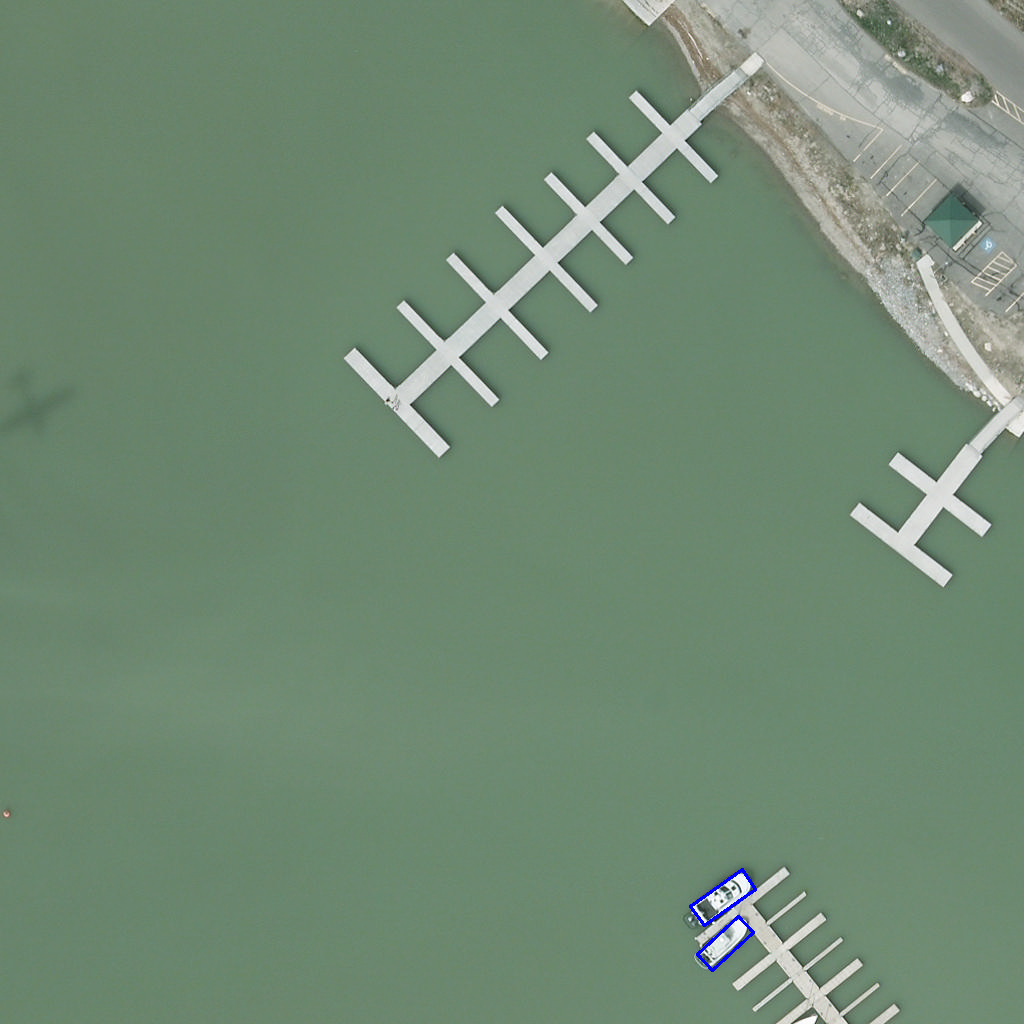
\includegraphics[trim={680pt 50pt 250pt 865pt},clip,width=\textwidth]{images/015Results/01abb_vs_obb/obb_ship.png}
        \caption{Labels: "Ship", OBB format}
        \label{fig:obb_ship}
    \end{subfigure}  
    \caption[Comparison of the bounding box formats of two different object classes]{Comparison of the bounding box formats of two different object classes (for full-sized images see \ref{fig:comparison_bb_format_fs}). \acrshort{obb} enclose objects much more accurately than \acrshort{abb}, as they include fewer irrelevant background areas. The reduced risk of overlap with neighbouring structures allows the model to extract more relevant object features and thus learn a more accurate representation of the classes (Own representation).
}
    \label{fig:comparison_bb_format}
\end{figure}
\todo{nicht nur erläutern was man sieht sondern auch was man daraus folgert (analyse) im Bildunterschrift}


Figure \ref{fig:comparison_bb_format} shows a comparison between \acrshort{obb} and \acrshort{abb} for different object classes. This difference is particularly clear in the truck example: in Figure \ref{fig:abb_truck}, \acrshort{abb} occupies a significantly larger area with approx. 1378 px than \acrshort{obb} in Figure \ref{fig:obb_truck} with approx. 967 px. When comparing highly rotated objects, such as the ships in Figure \ref{fig:abb_ship} and \ref{fig:obb_ship}, it can be seen that \acrshort{obb} encloses the object itself much more precisely and includes less of the surrounding area. Another advantage of \acrshort{obb} is the absence of overlaps between the boxes. For further examples, see Fig. \ref{fig:aab_obb_example_pics}. The line ‘ABB in OBB’ describes that the \acrshort{obb} model (\acrshort{YOLO}v9u) was trained with \acrshort{abb} bounding boxes. This means that the \acrshortpl{obb} in the \acrshort{VEDAI} dataset are converted to the bounding box format intended for \acrshort{YOLO}v9 (see \hyperlink{eq:yolov9u} {Equ.} in section \ref{sec:yolov9}) as \acrshort{abb} (i.e. with 8 coordinates that span an axis-parallel bounding box).
 

A comparison of all bounding box areas (see Figure \ref{fig:bbox_area}) shows that \acrshort{obb} is more compact on average (median \acrshort{abb}: approx. 1000 px, median \acrshort{obb}: >700 px). The \acrshort{abb} areas correspond almost exactly to the ‘ABB in OBB’ because the bounding boxes are almost identical; the only difference lies in the trained model and the calculations of the corners of the \acrshort{abb}. The bounding boxes occupy approximately 0.066\% of the total image area as \acrshort{obb} (approx. 700 px per box) and approximately 0.095\% as \acrshort{abb} (approx. 1000 px per box). This means that \acrshort{obb} is just below the lower limit for very small objects according to \citeauthor {Chen2017} \cite{Chen2017} (see section \ref{ch:state_of_research}) and are considered ‘very small objects’, while \acrshort{abb} is above the lower limit for small objects and is therefore considered a ‘small object’ (see \ref{ap:calc_bb_area_percent} for calculation).




\begin{figure}[htbp]
    \centering
    \includesvg[width=0.8\textwidth]{images/015Results/01abb_vs_obb/boxplot_areas.svg}
    \caption[Comparison of Bounding Box Area in pixels for \acrshort{abb}, \acrshort{obb}, abb in obb]{Comparison of Bounding Box Area in pixels for \acrshort{abb}, \acrshort{obb}, ABB in OBB. "ABB in OBB" means, that \acrlong{abb} converted to obb was used in the \acrshort{YOLO}v9u model with zero rotation. Due to their rotation-based adjustment, \acrshortpl{obb} are more compact than \acrshortpl{abb} and comprise less background. Since the calculation of ‘ABB in OBB’ areas yields almost identical values, it can be assumed that \acrshort{obb} models achieve higher performance due to more precise limitations (Own representation).}
    \label{fig:bbox_area}
\end{figure}


\begin{figure}[htbp]
    \centering
    \includesvg[width=0.8\textwidth]{images/015Results/01abb_vs_obb/abb_obb_best_val_on_val.svg}
    \caption[Comparison of \acrshort{mAP}@0.5--0.95 values for \acrshort{abb} and \acrshort{obb} (Best validation model on validation dataset)]{Comparison of \acrshort{mAP}@0.5--0.95 values for \acrshort{abb} and \acrshort{obb} (Best validation model on validation dataset). "ABB in OBB" means, that \acrlongpl{abb} converted to \acrshortpl{obb} was used in the \acrshort{YOLO}v9u model with zero rotation. \acrshort{abb} show a lower \acrshort{mAP}, presumably due to the model, while \acrshort{obb} are superior due to their better object adaptation. Notably, ‘ABB in OBB’ achieves higher values, which may indicate the strong rotation sensitivity of \acrshort{obb} (Own representation).}
    \label{fig:obb_abb_map50-95:val_on_val}
\end{figure}
The analysis of \acrshort{mAP}@0.5--0.95 of the best validation model on the validation dataset (Figure \ref{fig:obb_abb_map50-95:val_on_val}) shows that the \acrshort{obb} model performs better than the \acrshort{abb} model in all cases. All models used to evaluate the performance of \acrshort{obb} and \acrshort{abb} were trained exclusively on the basis of \acrshort{RGB} images. Interestingly, \acrshortpl{abb} achieves higher performance on the \acrshort{obb} model than the adapted \acrshort{obb} boxes within the same model (\acrshort{YOLO}v9u). The same phenomenon can also be observed on the test dataset (Figure \ref{fig:obb_abb_map50-95:val_on_test}), so that \acrshort{abb} in conjunction with the \acrshort{obb} model delivers better results. It is striking that for the \acrshort{abb}-based models (both \acrshort{abb} and ‘ABB in OBB’), fold 1 always achieved the best value on the validation dataset, while for the \acrshort{obb} model, fold 0 delivered the best results there (see Table \ref{tab:best_folds_area} and Fig. \ref{fig:obb_abb_map50-95:val_on_val}). The results of the respective folds with the highest \acrshort{mAP}@0.5--0.95 value from Fig. \ref{fig:obb_abb_map50-95:val_on_val} are marked by the red dot in Figure \ref{fig:obb_abb_map50-95:val_on_test}. According to Table \ref{tab:best_folds_area} and Fig. \ref{fig:obb_abb_map50-95:val_on_val}, fold 1 achieved the highest \acrshort{mAP} value in the \acrshort{abb} model. However, on the test fold, this fold 1 only achieved the lower quantile, as can be seen in Fig. \ref{fig:obb_abb_map50-95:val_on_test} at the red dot.


\begin{table}[h]
\centering
\begin{tabular}{l c c}
\hline
\textbf{Model} & \textbf{Best mAP Fold (Validation)} & \textbf{Best mAP Fold (Test)} \\ 
\hline
abb &  1 & 1 \\
obb &  0 & 0 \\
abb in obb &  1 & 1 \\
\hline
\end{tabular}
\caption{Best fold per model at Bounding Box format}
\label{tab:best_folds_area}
\end{table}


The effects of the different rotations of the detected objects can be seen in Figure \ref{fig:aab_obb_example_pics} using the class \texttt{plane} as an example. The bounding boxes differ significantly in terms of their rotation angles between the three models. Deviations in the overlap of the detected bounding boxes with the ground truth annotations, on the other hand, occur much less frequently, which explains the higher \acrshort{mAP} performance of the \acrshort{abb}-based models. Other notable features, such as the difficulties in separating objects from the background, are discussed in the following sections.

Due to the lower probability of overlap errors and the more precise object contouring, the \acrshort{obb} format was selected for performing the permutation tests.


\begin{figure}[htbp]
    \centering
    \includesvg[width=0.8\textwidth]{images/015Results/01abb_vs_obb/aab_obb_best_val_on_test.svg}
    \caption[Comparison of \acrshort{mAP}@0.5--0.95 values for \acrshort{abb} and \acrshort{obb} (Best validation model on test dataset)]{Comparison of \acrshort{mAP}@0.5--0.95 values for \acrshort{abb} and \acrshort{obb} (Best validation model on test dataset). "ABB in OBB" means, that \acrlongpl{abb} converted to \acrshortpl{obb} was used in the \acrshort{YOLO}v9u model with zero rotation. The red dot is the fold, that has the best \acrshort{mAP}50-95 at the validation dataset (see fig. \ref{fig:obb_abb_map50-95:val_on_val}).  On the test dataset, \acrshort{abb} achieves poorer results, presumably due to model limitations, while \acrshort{obb} achieves significantly better performance due to more precise object boundaries. The ‘ABB in OBB’ configuration shows the best performance, as even small rotation deviations in the \acrshort{obb} model strongly influence the \acrshort{mAP} and the model's \acrshort{GT} \acrshort{BB} are significantly larger (Own representation). }
    \label{fig:obb_abb_map50-95:val_on_test}
\end{figure}

%##########################################################################
%##########################################################################

\begin{figure}[h!]
\centering
\renewcommand{\arraystretch}{1.2} % mehr Platz zwischen Zeilen
\setlength{\tabcolsep}{2pt} % weniger Platz zwischen Spalten
\begin{tabularx}{\textwidth}{c|*{9}{X}}
    & \textbf{Car}
    & \textbf{Truck}
    & \textbf{Camping Car}
    & \textbf{Tractor}
    & \textbf{Plane}
    & \textbf{Ship}
    & \textbf{Vehicle}
    & \textbf{Pick-Up}
    & \textbf{Van} \\ \hline
    \rotatebox{90}{\textbf{\acrshort{GT} (\acrshort{abb})}} 
    %Car
    & 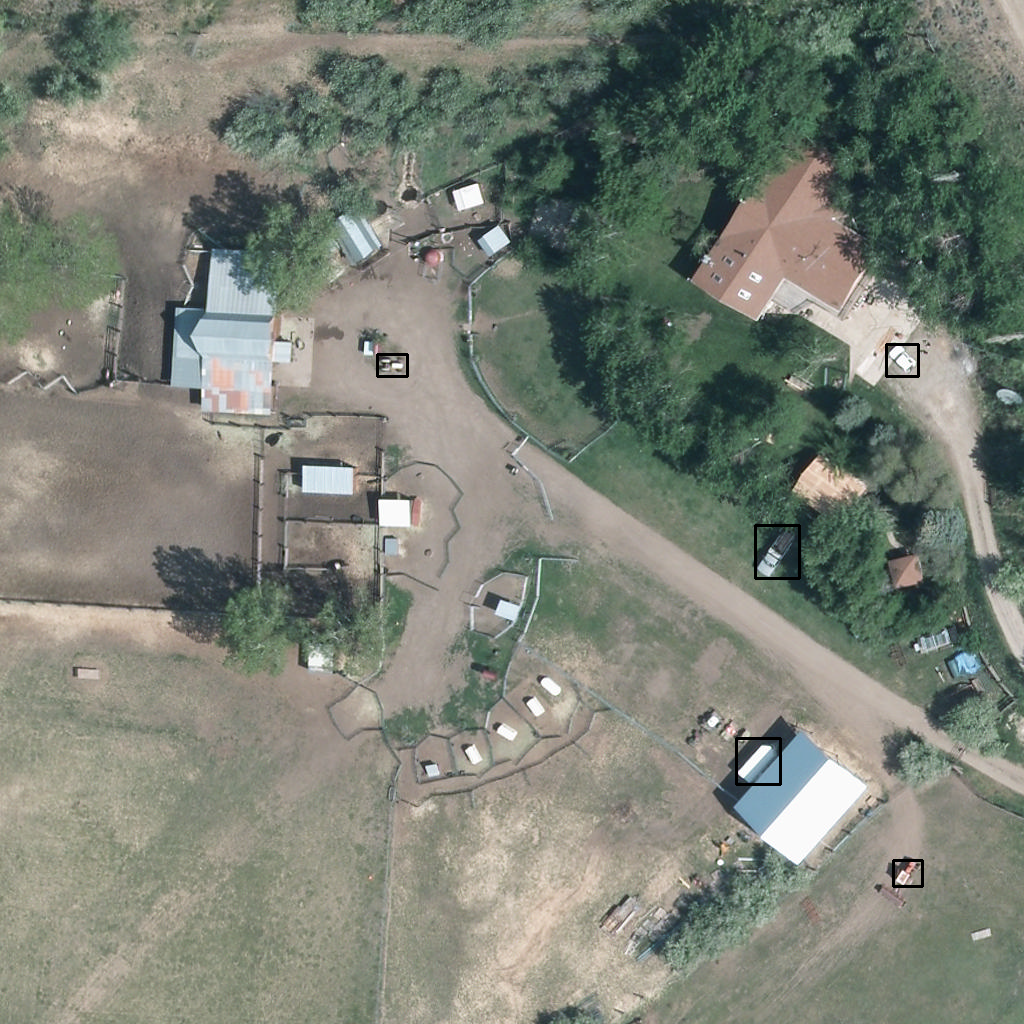
\includegraphics[trim={880pt 630pt 70pt 330pt},clip,width=\linewidth]{images/015Results/01abb_vs_obb/comp_images/ground_truth_abb/523.png}
    %Truck
    & 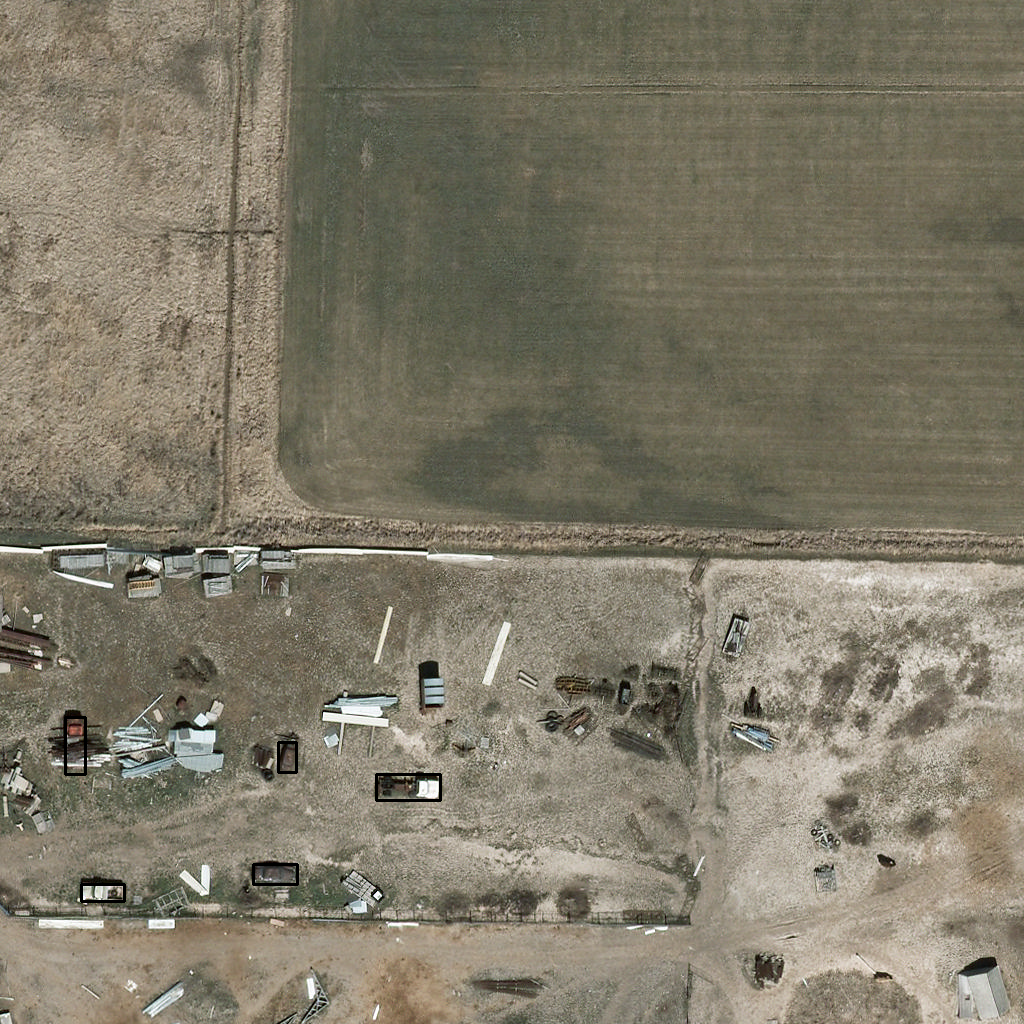
\includegraphics[trim={360pt 200pt 540pt 715pt},clip,width=\linewidth]{images/015Results/01abb_vs_obb/comp_images/ground_truth_abb/212.png}
    %Camping Car
    & 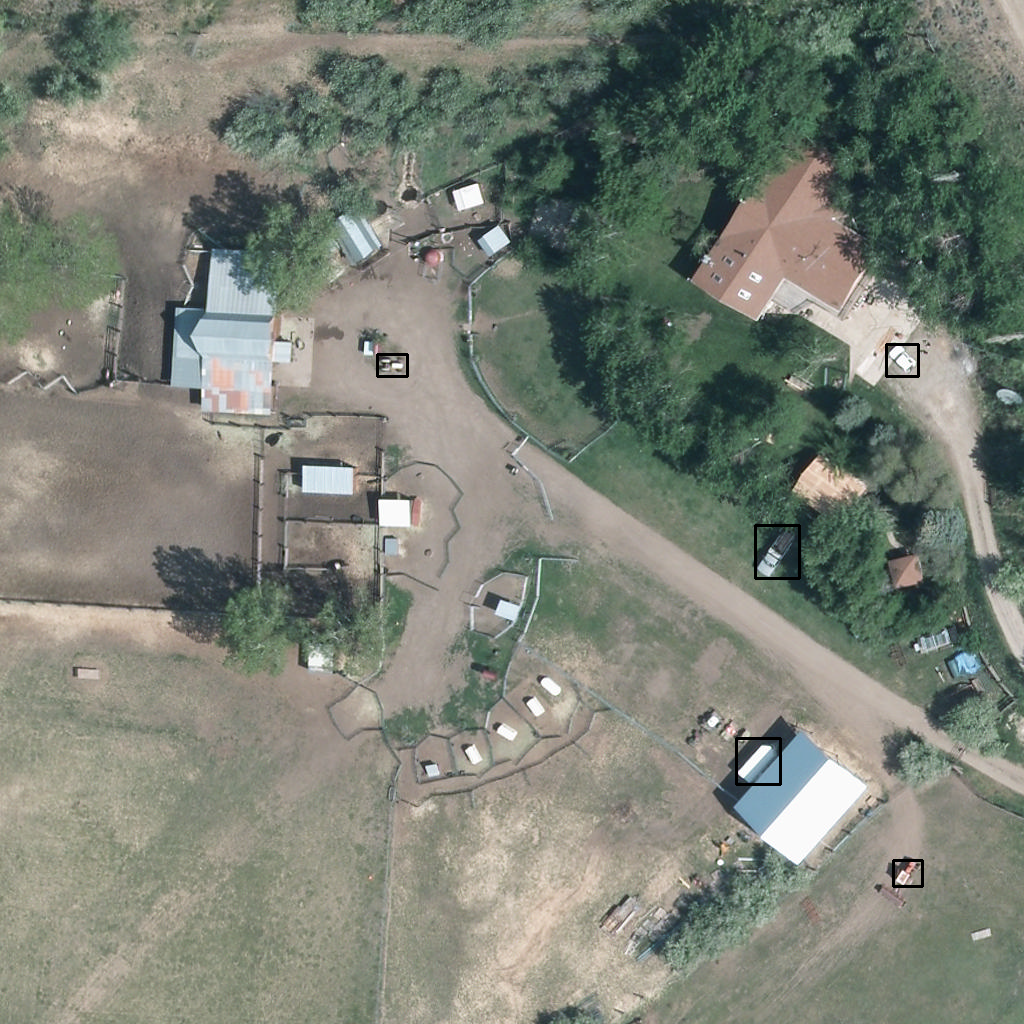
\includegraphics[trim={730pt 220pt 200pt 720pt},clip,width=\linewidth]{images/015Results/01abb_vs_obb/comp_images/ground_truth_abb/523.png}
    %Tractor
    & 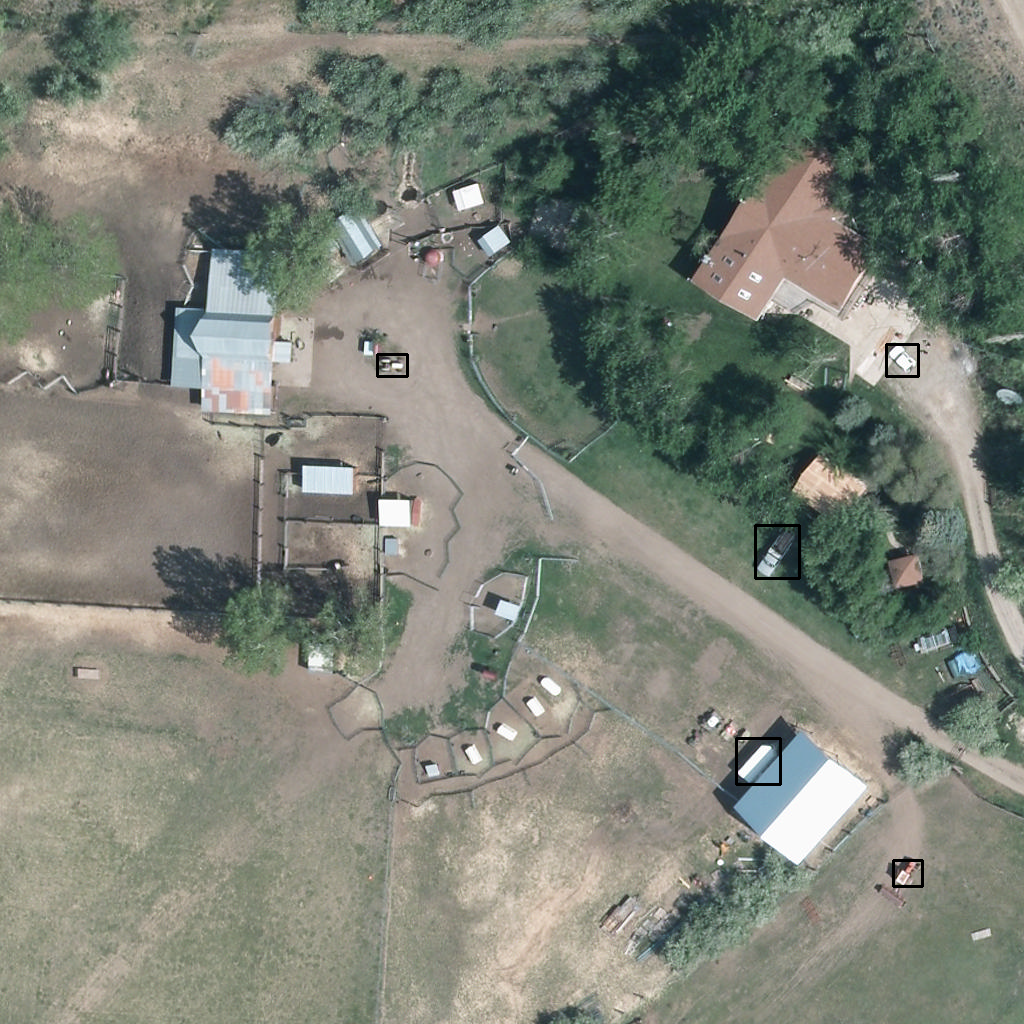
\includegraphics[trim={850pt 110pt 80pt 830pt},clip,width=\linewidth]{images/015Results/01abb_vs_obb/comp_images/ground_truth_abb/523.png}
    %Plane
    &  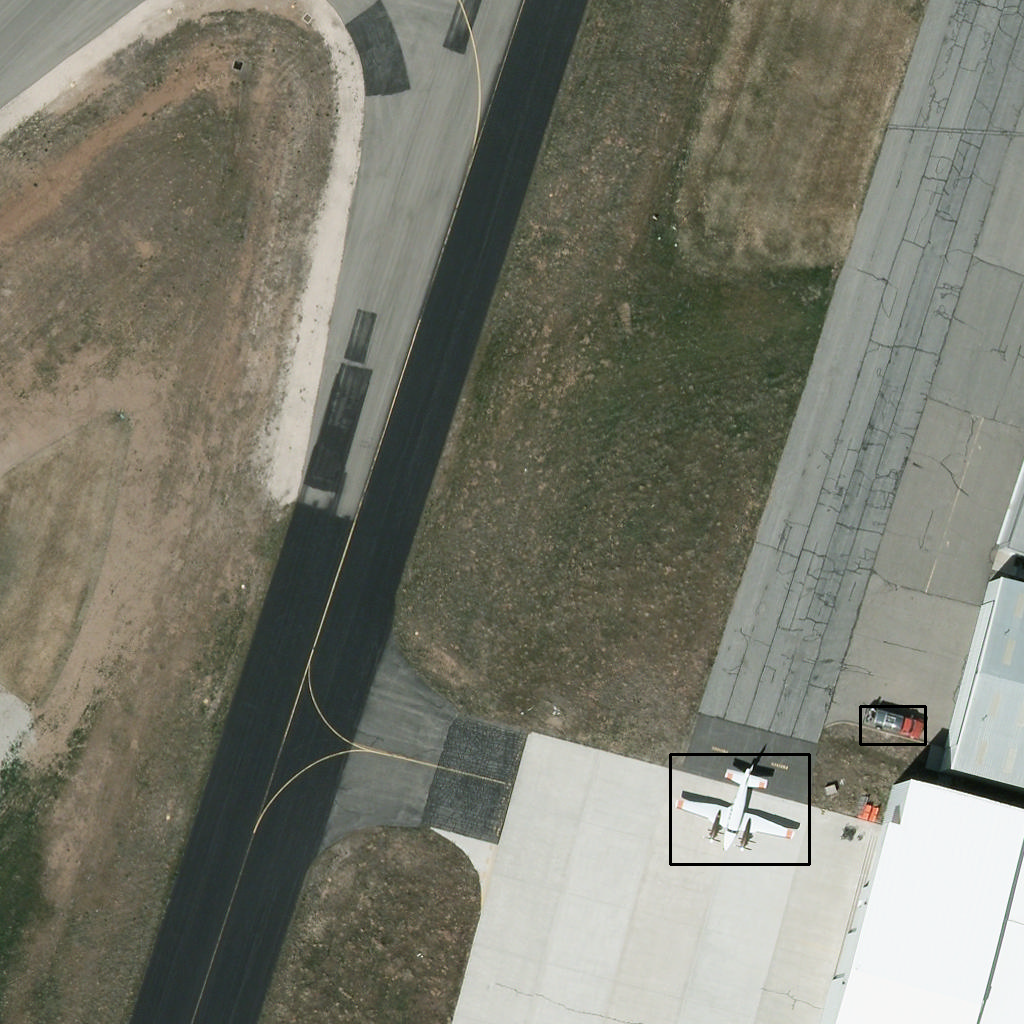
\includegraphics[trim={650pt 120pt 170pt 720pt},clip,width=\linewidth]{images/015Results/01abb_vs_obb/comp_images/ground_truth_abb/487.png}
    %Ship
    & 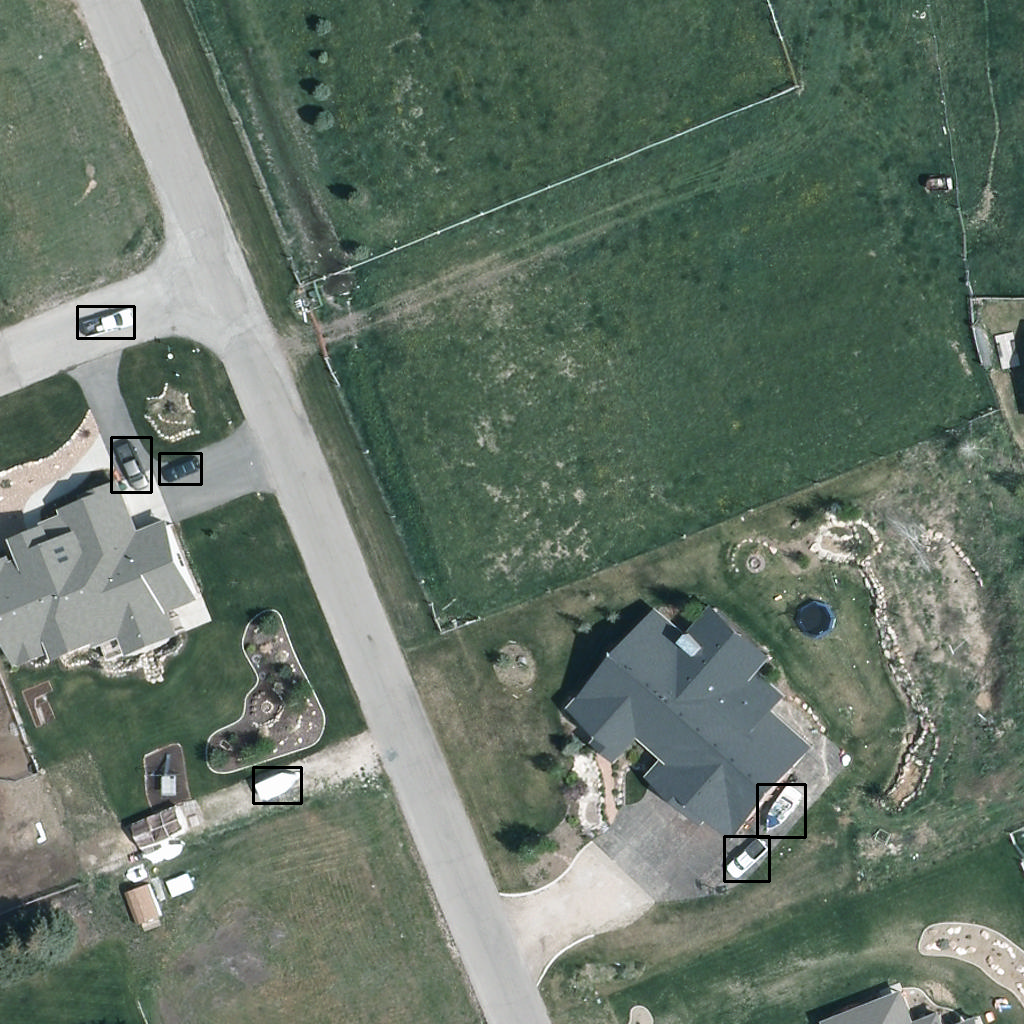
\includegraphics[trim={230pt 200pt 680pt 725pt},clip,width=\linewidth]{images/015Results/01abb_vs_obb/comp_images/ground_truth_abb/509.png}
    %vehicle
    & 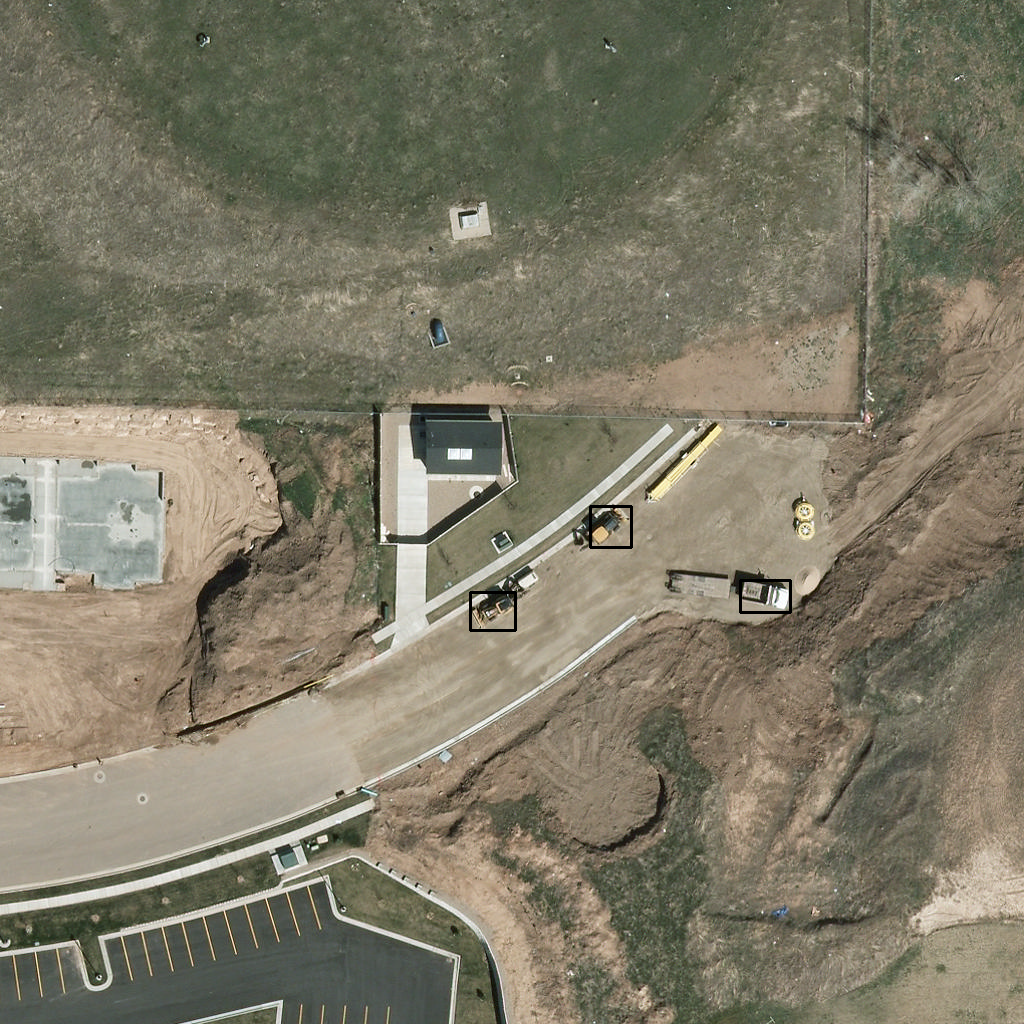
\includegraphics[trim={440pt 360pt 460pt 555pt},clip,width=\linewidth]{images/015Results/01abb_vs_obb/comp_images/ground_truth_abb/427.png}
    %Pick Up
    & 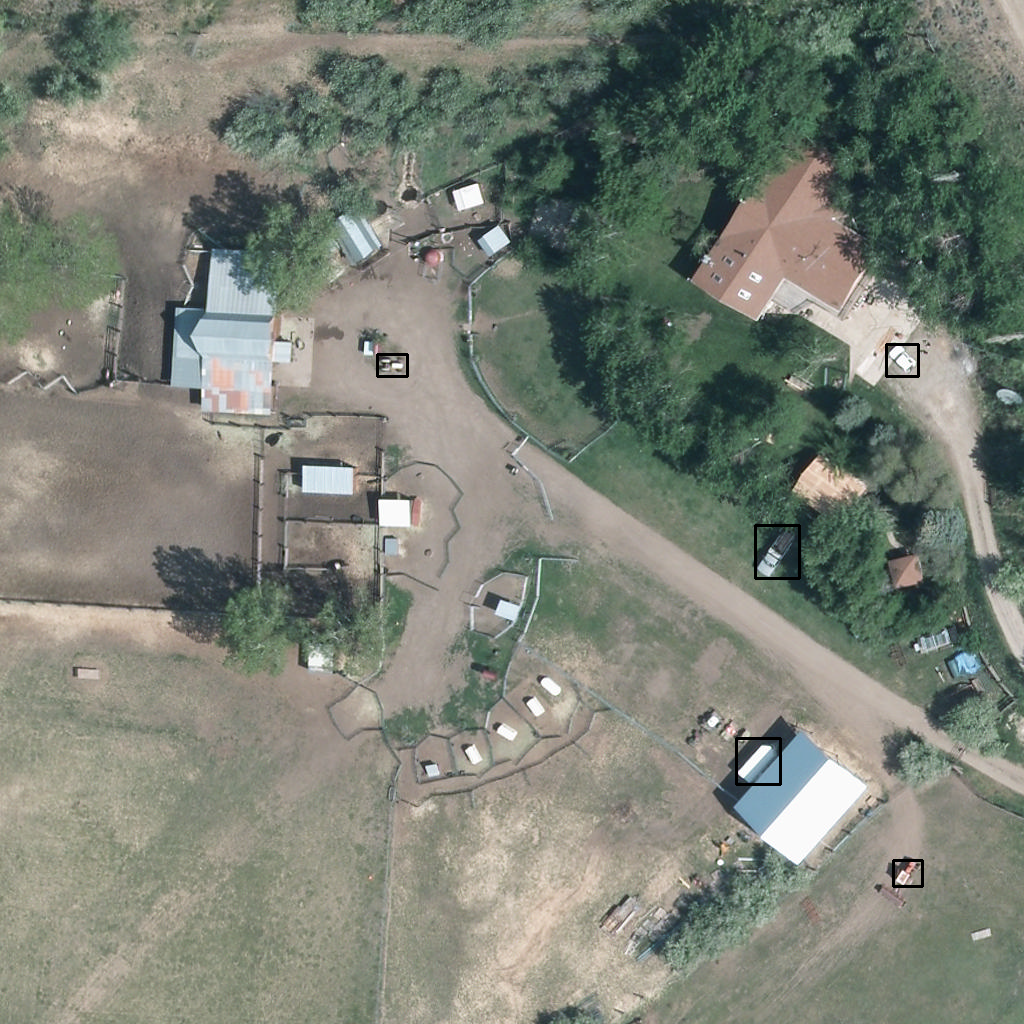
\includegraphics[trim={740pt 420pt 180pt 510pt},clip,width=\linewidth]{images/015Results/01abb_vs_obb/comp_images/ground_truth_abb/523.png}
    %Van
    & 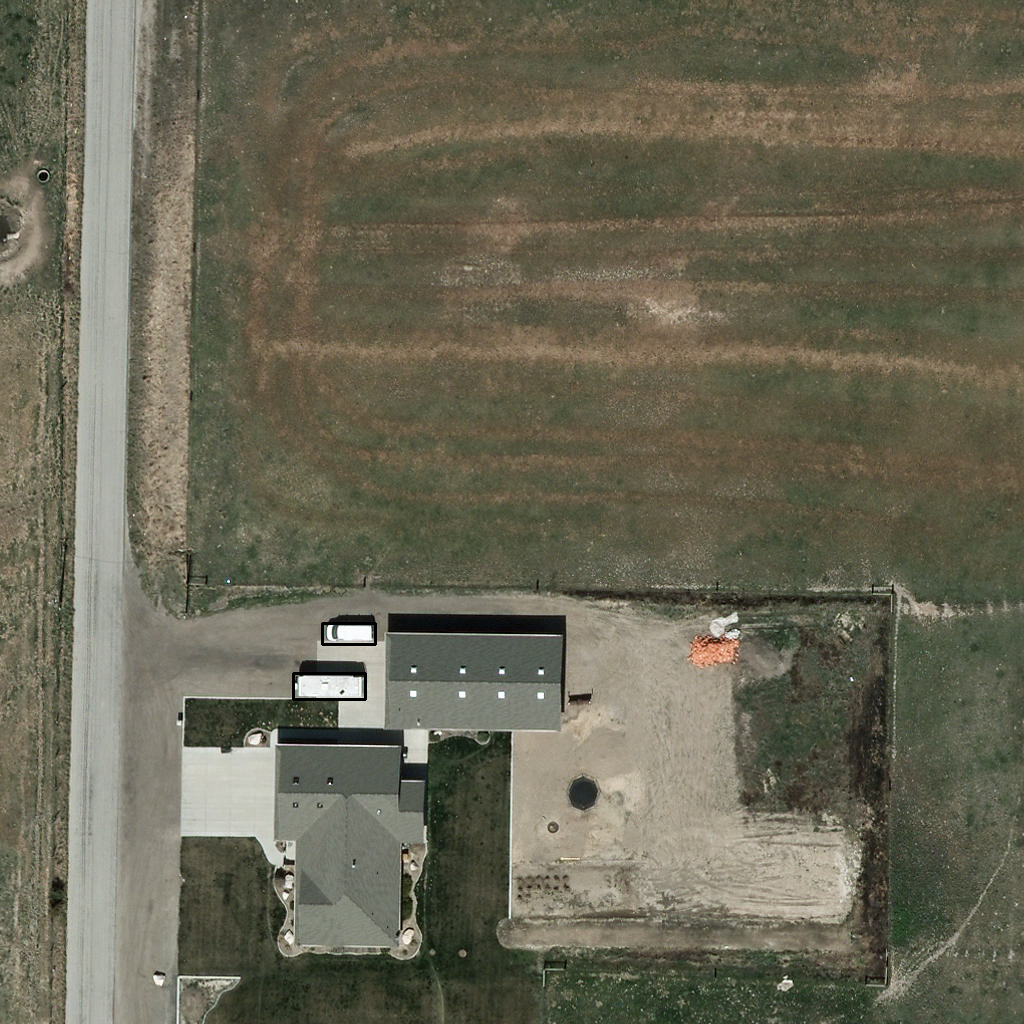
\includegraphics[trim={300pt 355pt 610pt 570pt},clip,width=\linewidth]{images/015Results/01abb_vs_obb/comp_images/ground_truth_abb/198.png} \\ \hline

    \rotatebox{90}{\textbf{\acrshort{GT} (\acrshort{obb})}} 
    %Car
    & 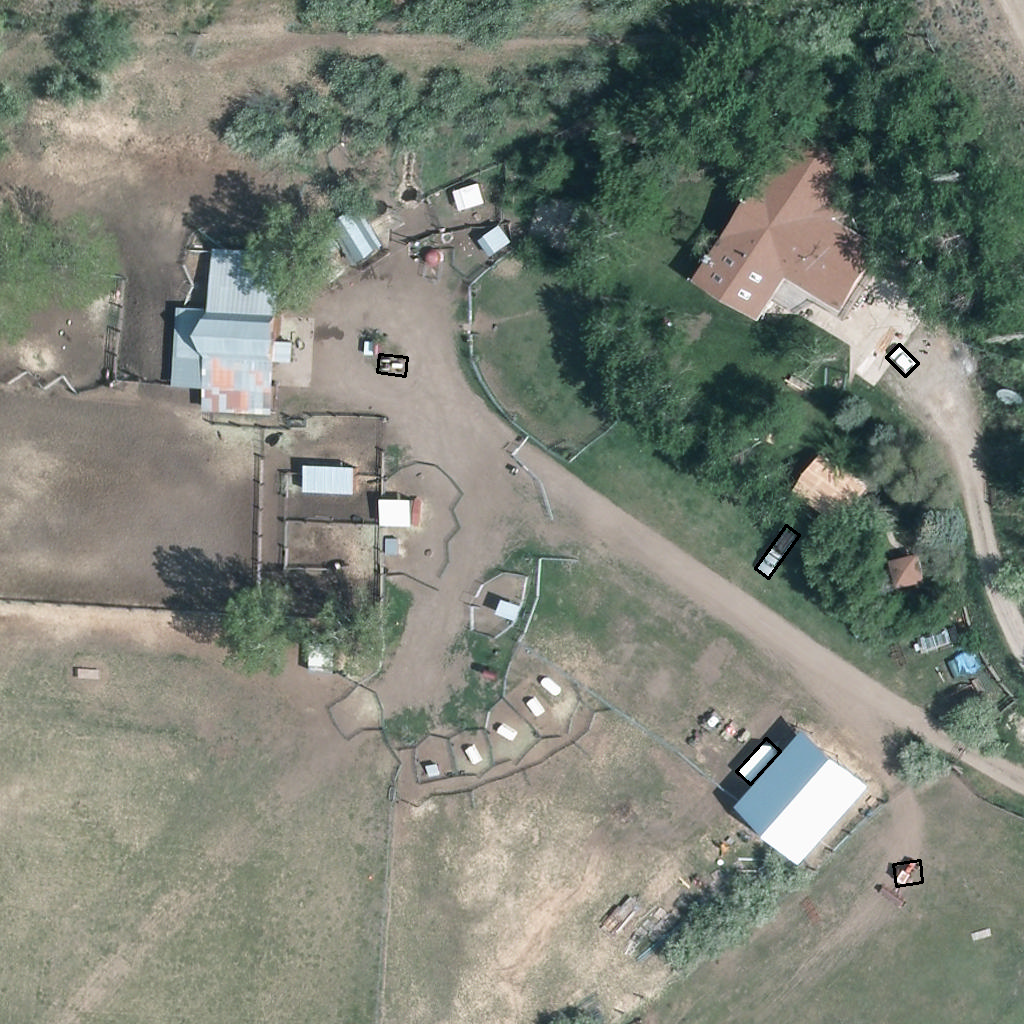
\includegraphics[trim={880pt 630pt 70pt 330pt},clip,width=\linewidth]{images/015Results/01abb_vs_obb/comp_images/ground_truth_obb/523.png}
    %Truck
    & 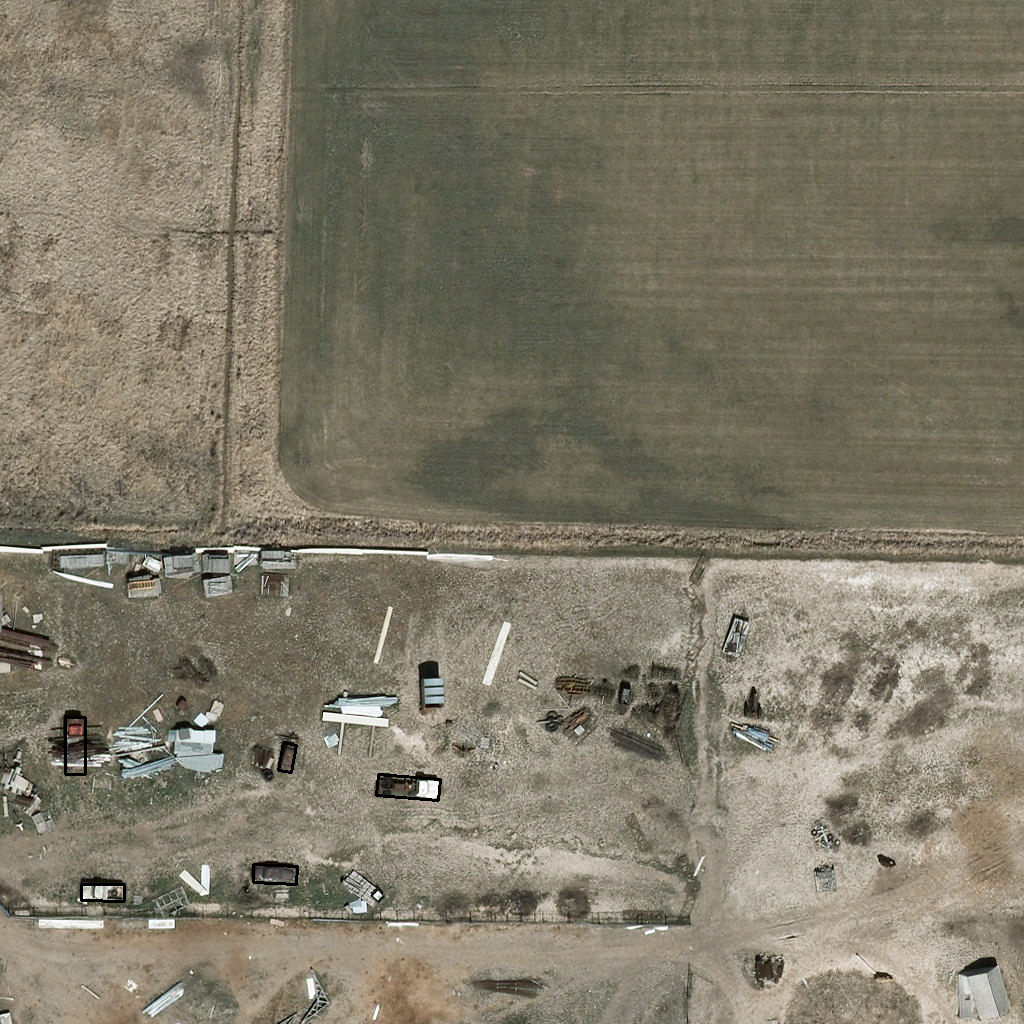
\includegraphics[trim={360pt 200pt 540pt 715pt},clip,width=\linewidth]{images/015Results/01abb_vs_obb/comp_images/ground_truth_obb/212.png}
    %Camping Car
    & 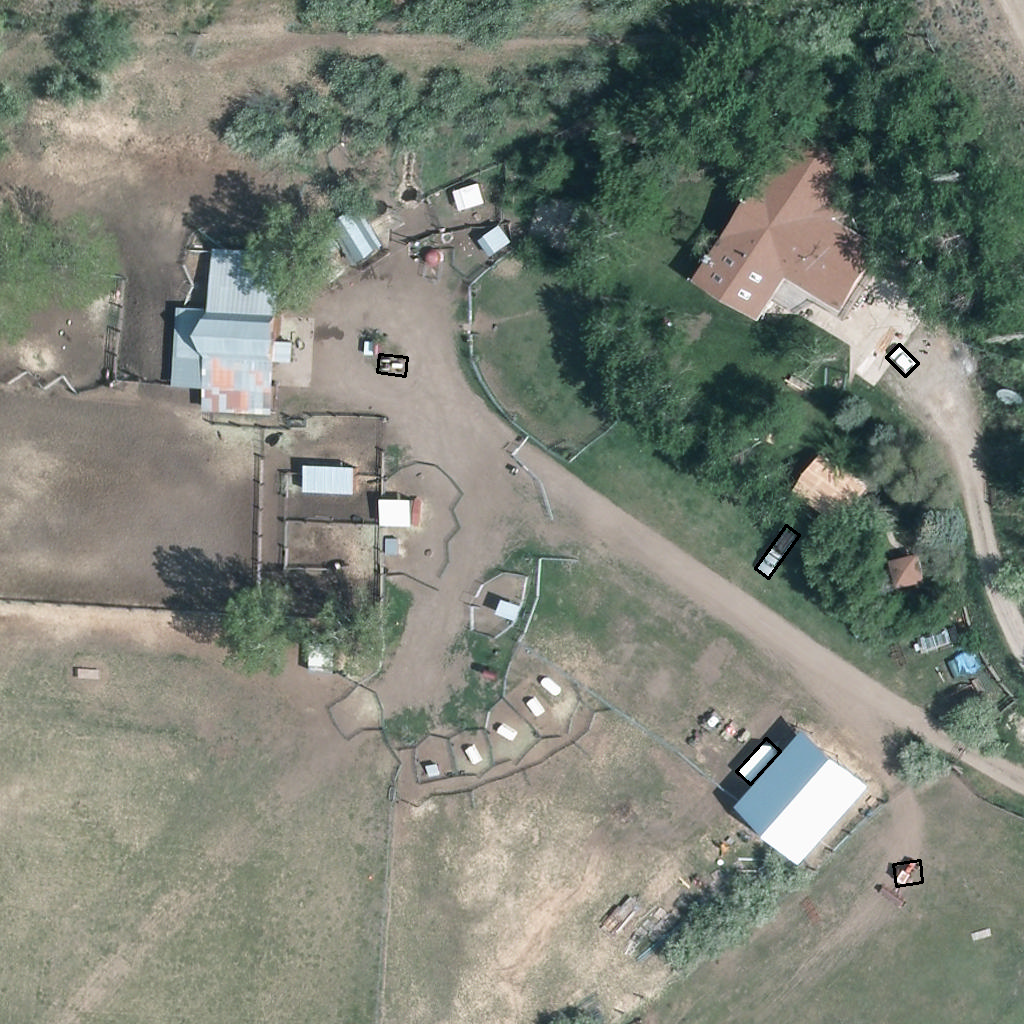
\includegraphics[trim={730pt 220pt 200pt 720pt},clip,width=\linewidth]{images/015Results/01abb_vs_obb/comp_images/ground_truth_obb/523.png}
    %Tractor
    & 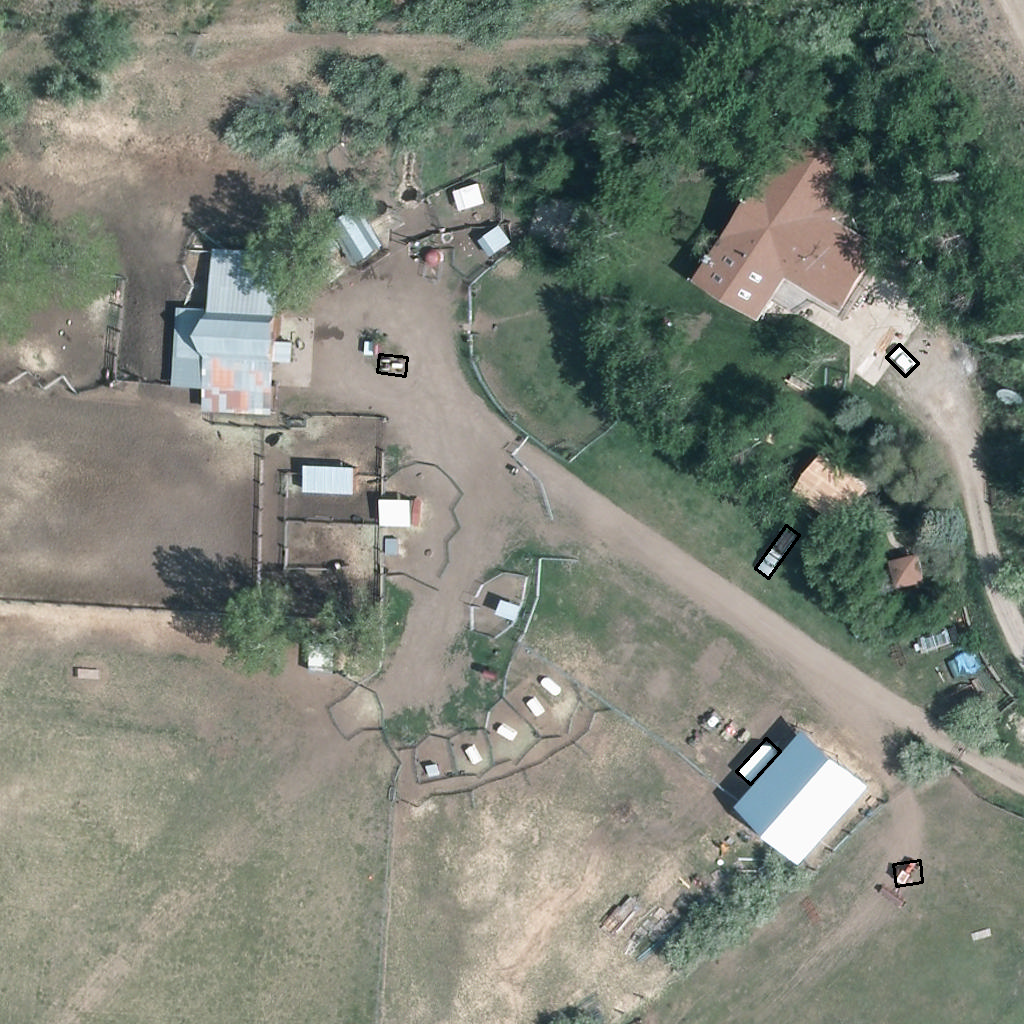
\includegraphics[trim={850pt 110pt 80pt 830pt},clip,width=\linewidth]{images/015Results/01abb_vs_obb/comp_images/ground_truth_obb/523.png}
    %Plane
    &  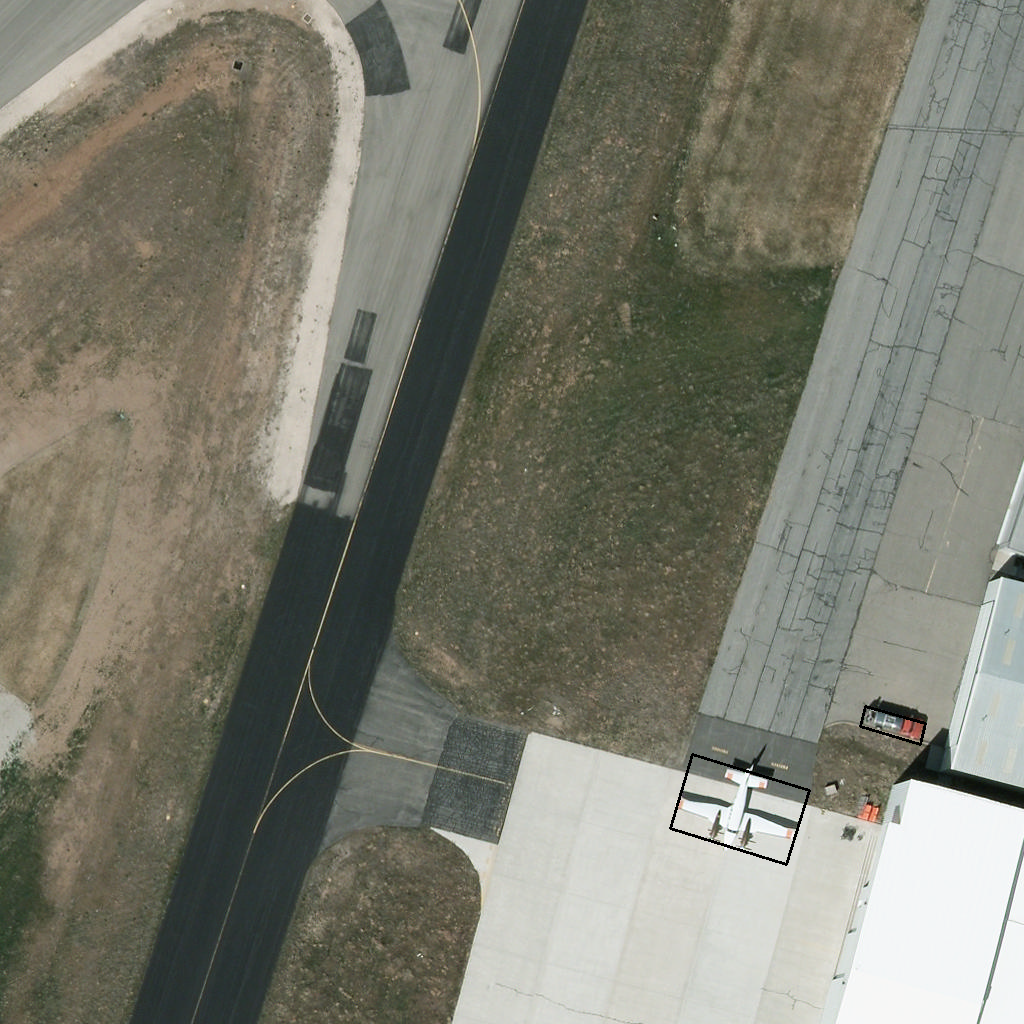
\includegraphics[trim={650pt 120pt 170pt 720pt},clip,width=\linewidth]{images/015Results/01abb_vs_obb/comp_images/ground_truth_obb/487.png}
    %Ship
    & 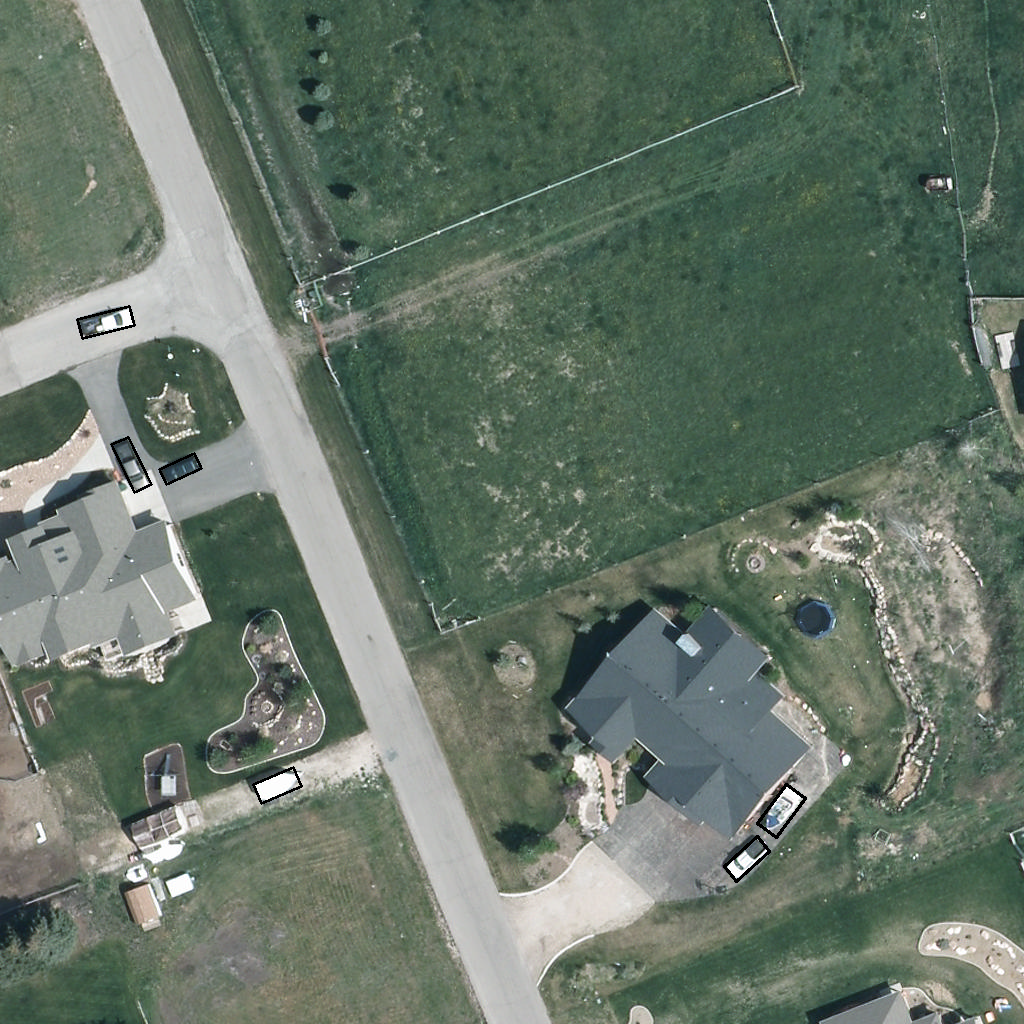
\includegraphics[trim={230pt 200pt 680pt 725pt},clip,width=\linewidth]{images/015Results/01abb_vs_obb/comp_images/ground_truth_obb/509.png}
    %vehicle
    & 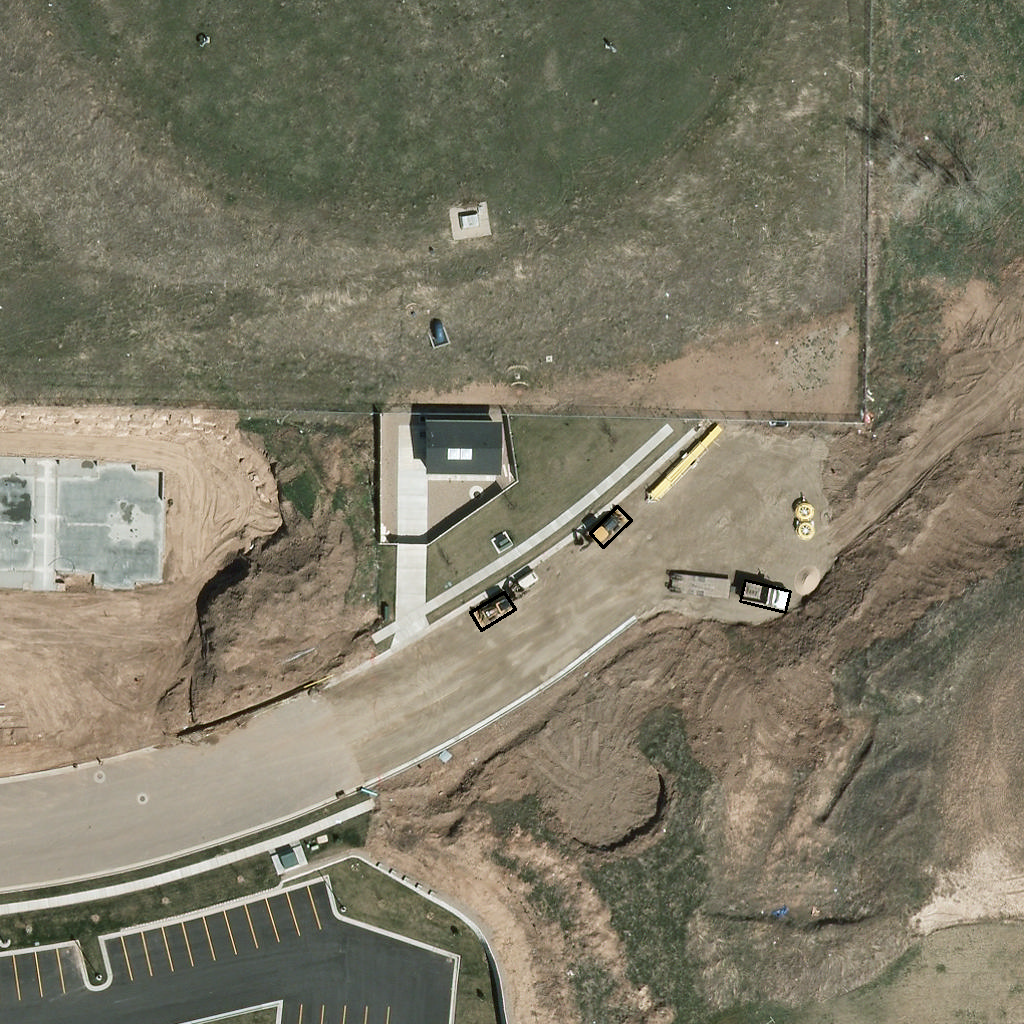
\includegraphics[trim={440pt 360pt 460pt 555pt},clip,width=\linewidth]{images/015Results/01abb_vs_obb/comp_images/ground_truth_obb/427.png}
    %Pick Up
    & 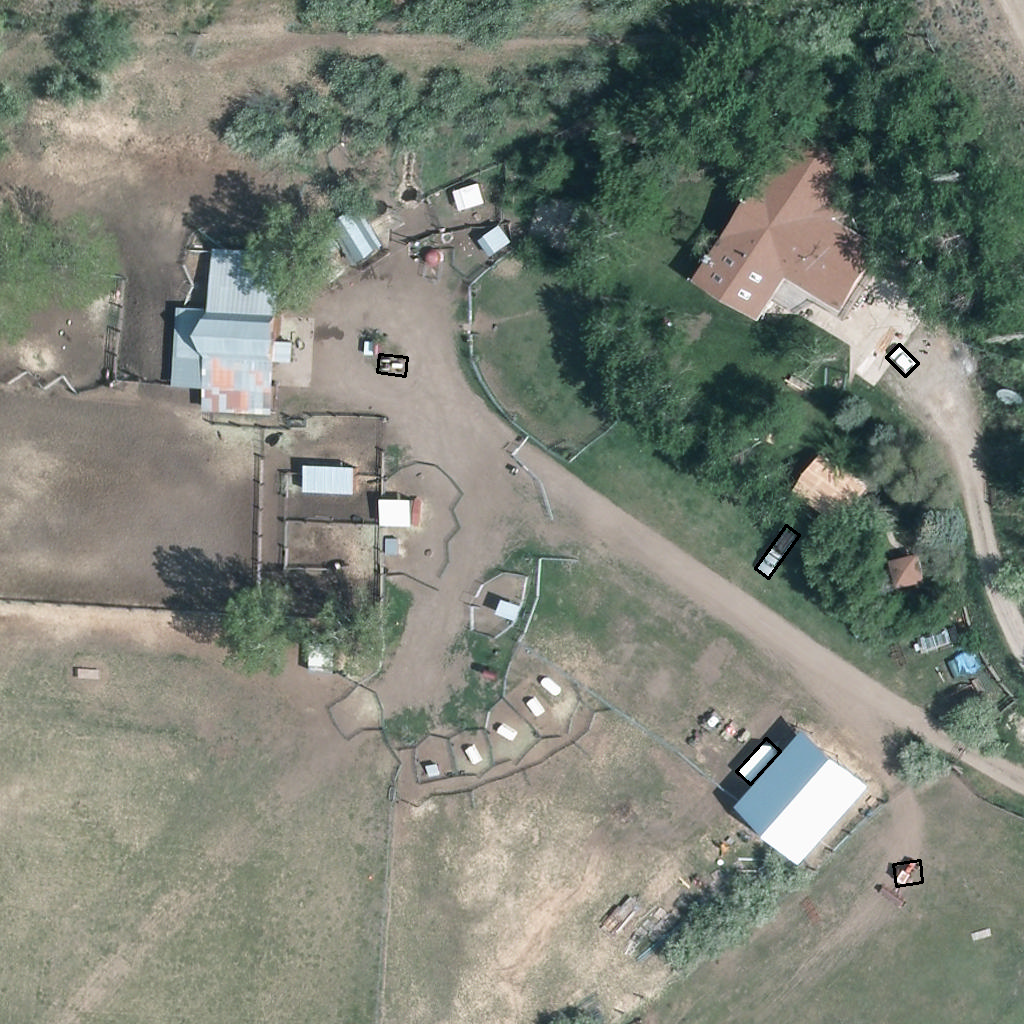
\includegraphics[trim={740pt 420pt 180pt 510pt},clip,width=\linewidth]{images/015Results/01abb_vs_obb/comp_images/ground_truth_obb/523.png}
    %Van
    & 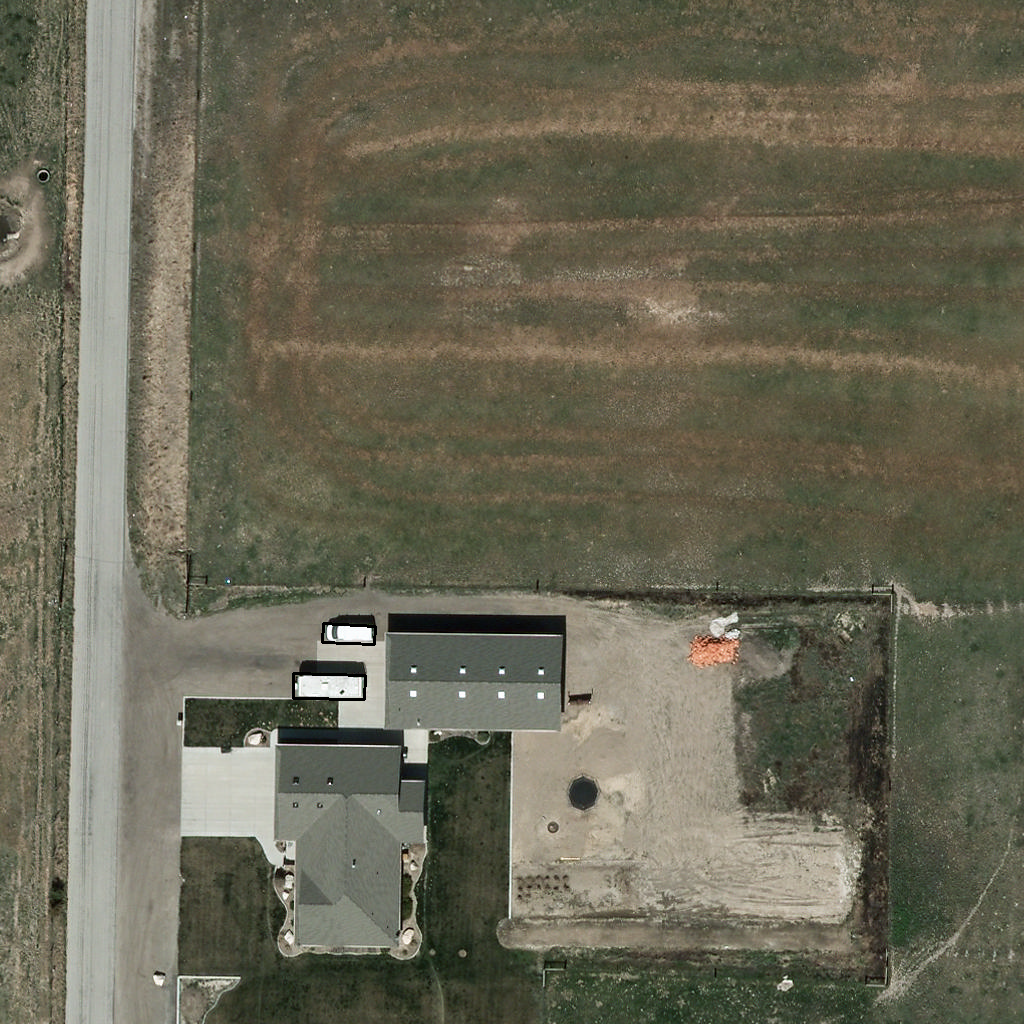
\includegraphics[trim={300pt 355pt 610pt 570pt},clip,width=\linewidth]{images/015Results/01abb_vs_obb/comp_images/ground_truth_obb/198.png} \\ \hline
    \rotatebox{90}{\textbf{\acrshort{abb}}} 
    %Car
    & 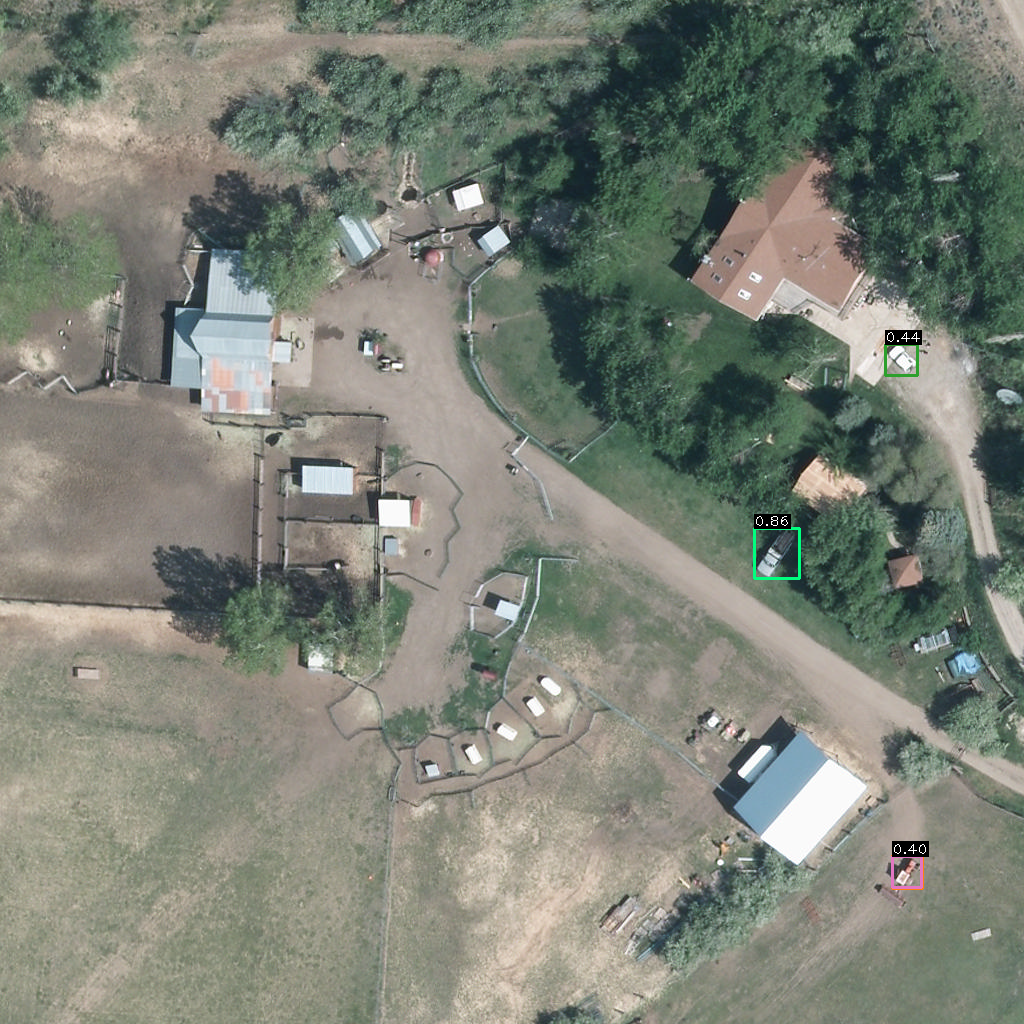
\includegraphics[trim={880pt 630pt 70pt 330pt},clip,width=\linewidth]{images/015Results/01abb_vs_obb/comp_images/abb/523.png}
    %Truck
    & 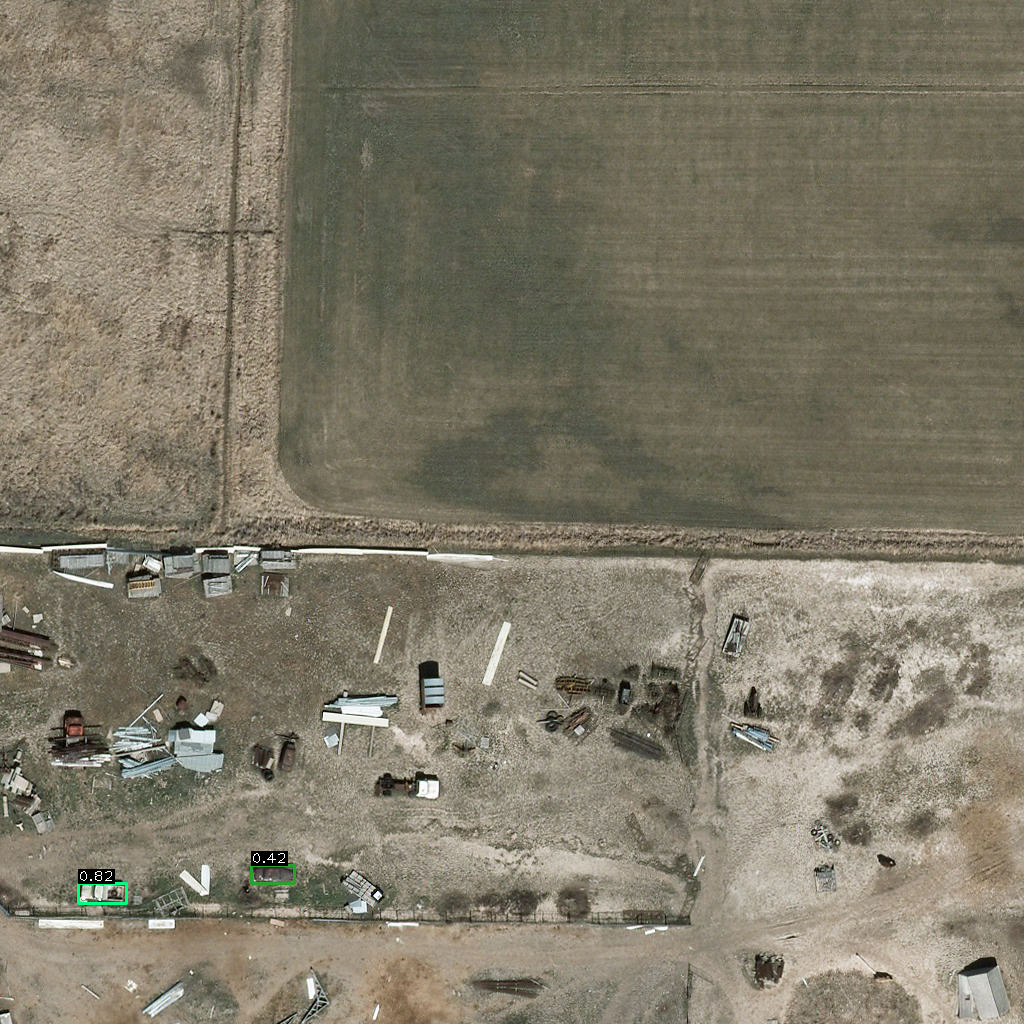
\includegraphics[trim={360pt 200pt 540pt 715pt},clip,width=\linewidth]{images/015Results/01abb_vs_obb/comp_images/abb/212.png}
    %Camping Car
    & 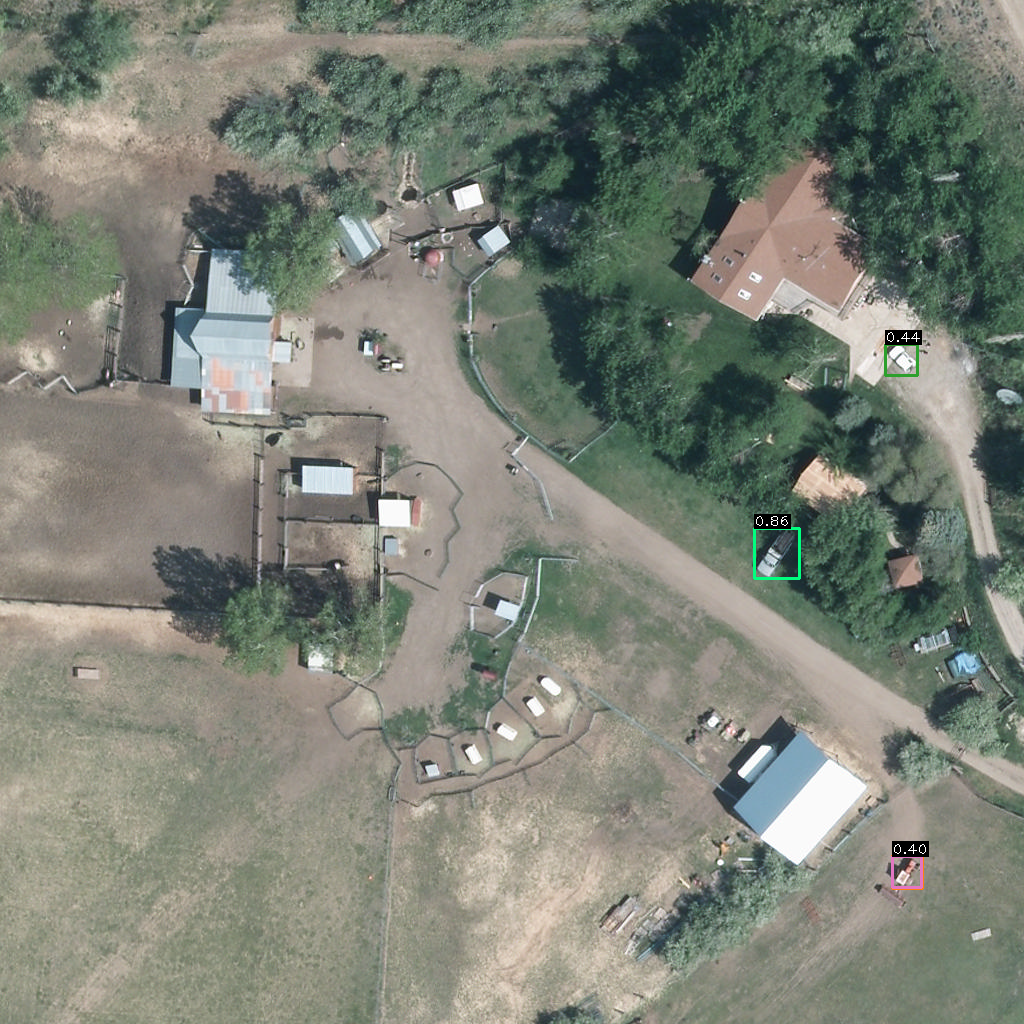
\includegraphics[trim={730pt 220pt 200pt 720pt},clip,width=\linewidth]{images/015Results/01abb_vs_obb/comp_images/abb/523.png}
    %Tractor
    & 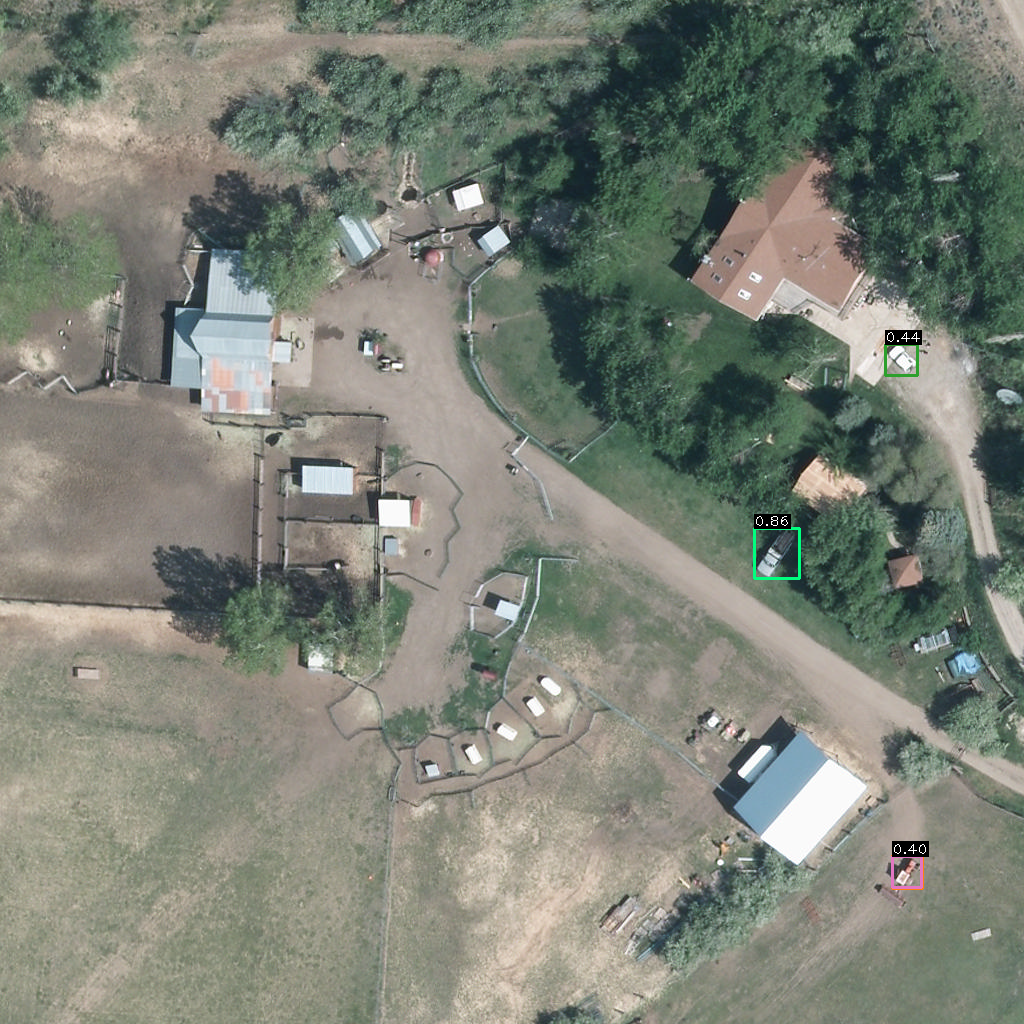
\includegraphics[trim={850pt 110pt 80pt 830pt},clip,width=\linewidth]{images/015Results/01abb_vs_obb/comp_images/abb/523.png}
    %Plane
    &  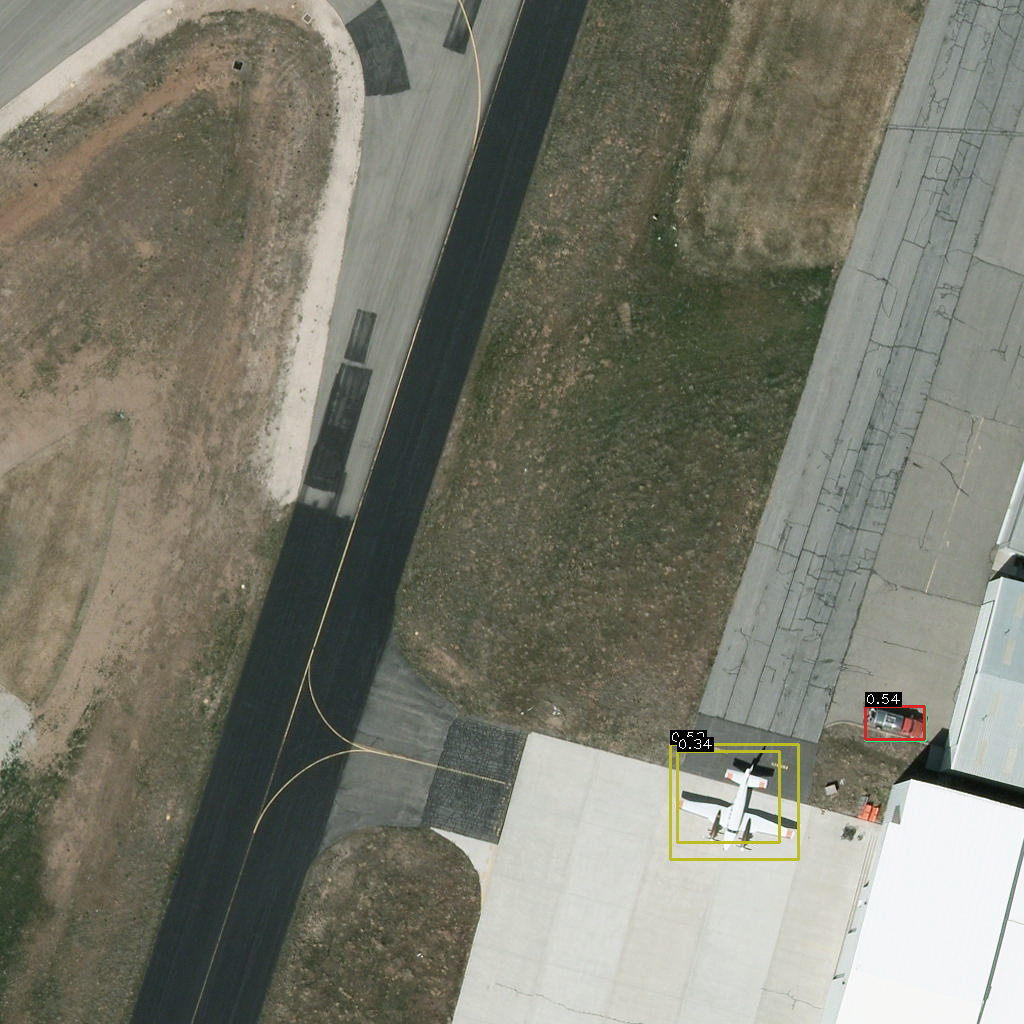
\includegraphics[trim={650pt 120pt 170pt 720pt},clip,width=\linewidth]{images/015Results/01abb_vs_obb/comp_images/abb/487.png}
    %Ship
    & 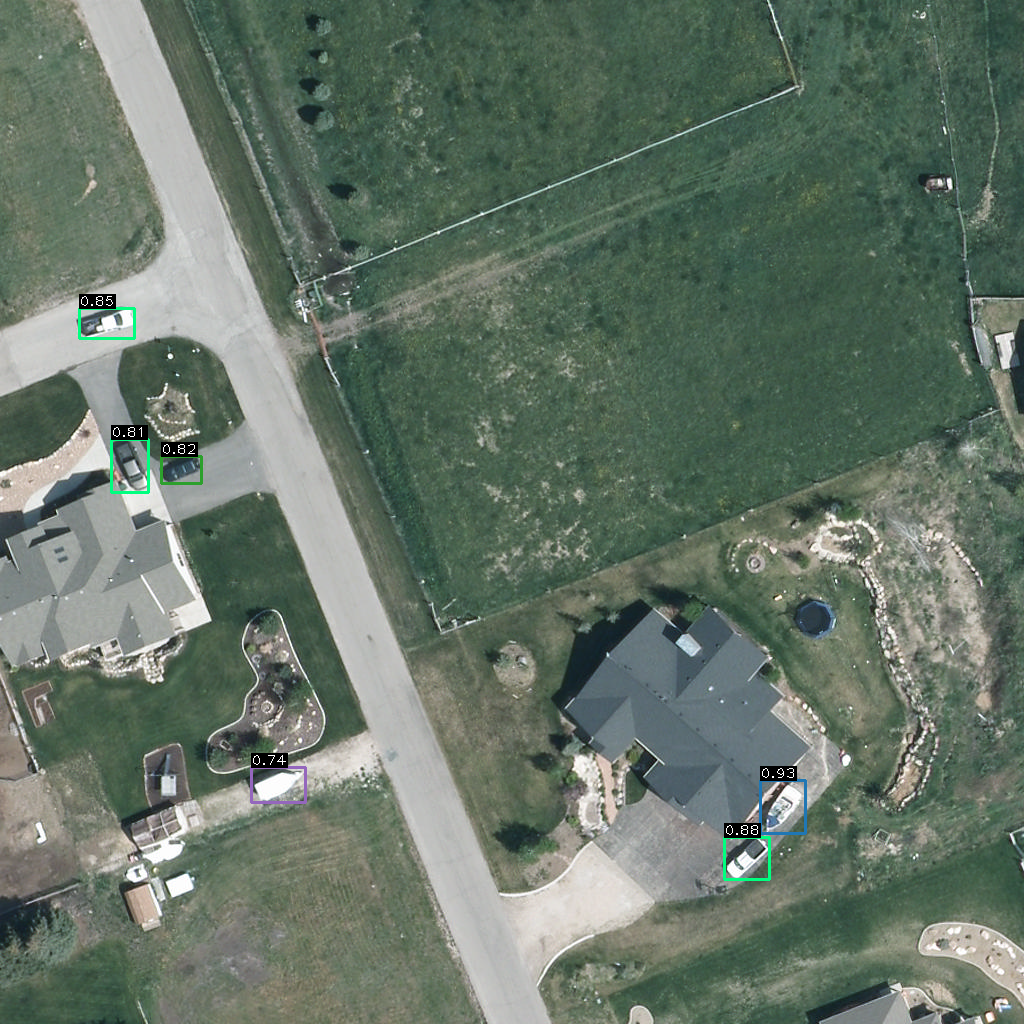
\includegraphics[trim={230pt 200pt 680pt 725pt},clip,width=\linewidth]{images/015Results/01abb_vs_obb/comp_images/abb/509.png}
    %vehicle
    & 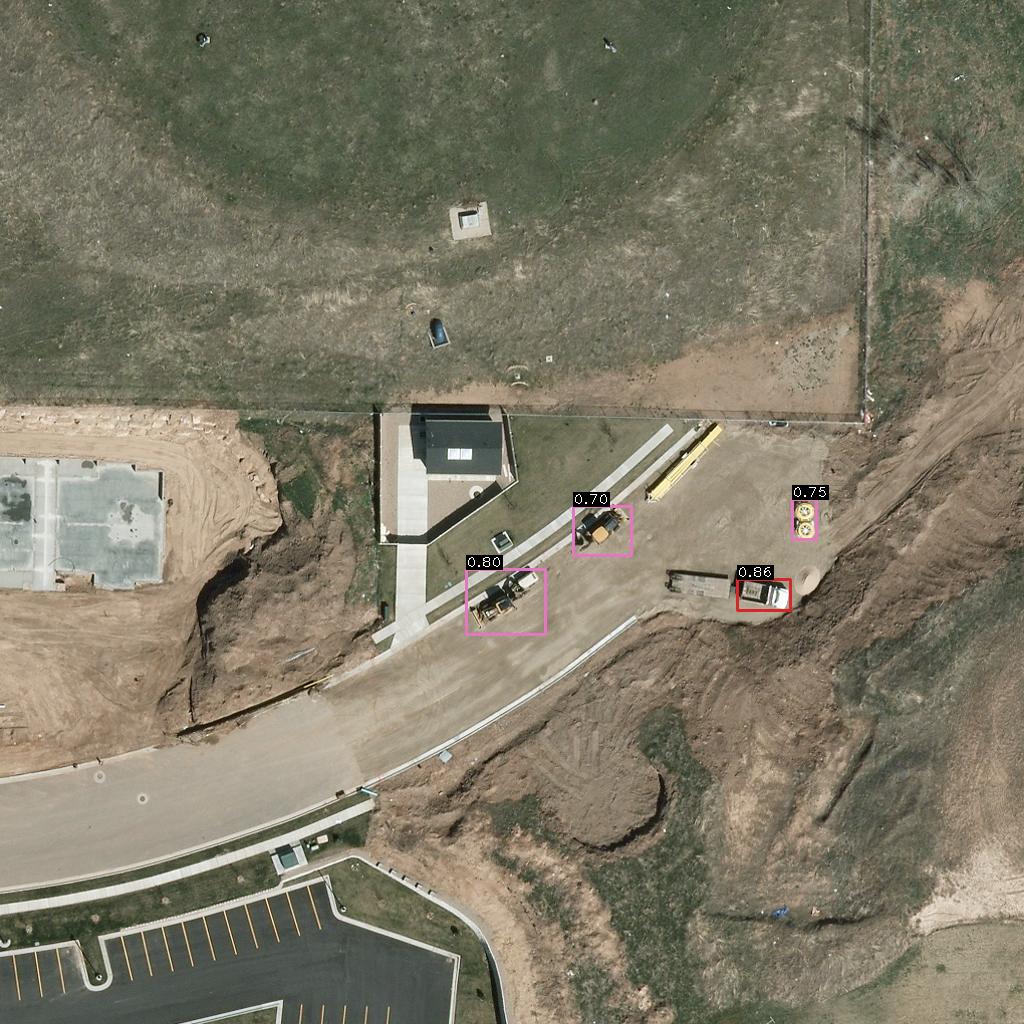
\includegraphics[trim={440pt 360pt 460pt 555pt},clip,width=\linewidth]{images/015Results/01abb_vs_obb/comp_images/abb/427.png}
    %Pick Up
    & 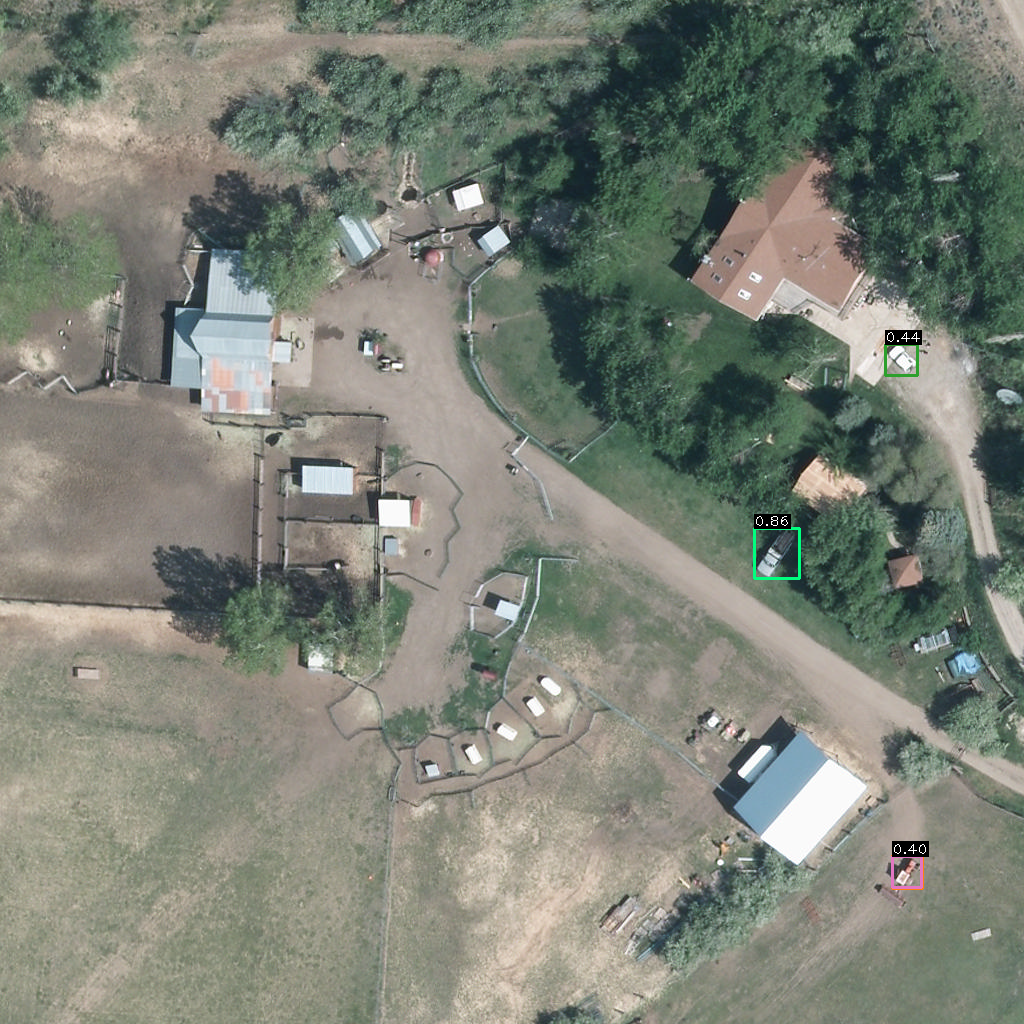
\includegraphics[trim={740pt 420pt 180pt 510pt},clip,width=\linewidth]{images/015Results/01abb_vs_obb/comp_images/abb/523.png}
    %Van
    & 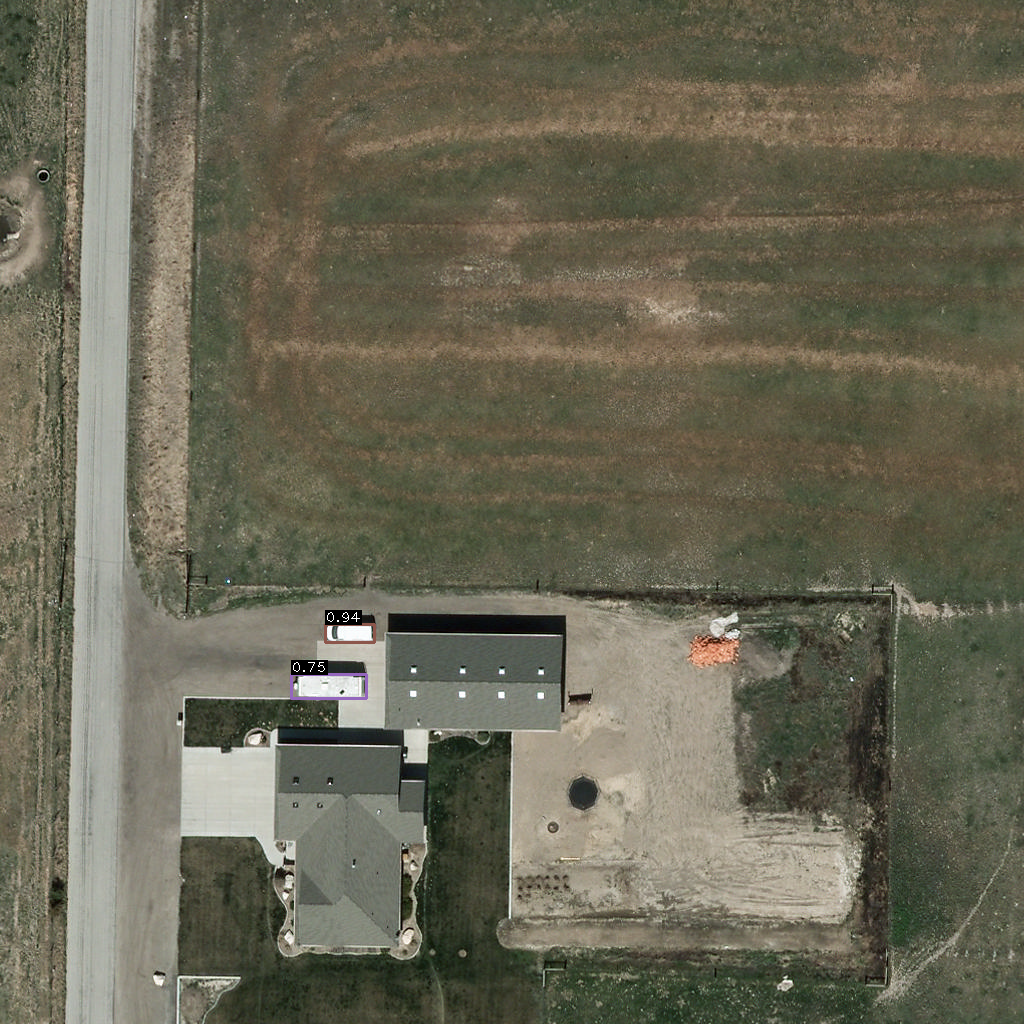
\includegraphics[trim={300pt 355pt 610pt 570pt},clip,width=\linewidth]{images/015Results/01abb_vs_obb/comp_images/abb/198.png} \\ \hline
    \rotatebox{90}{\textbf{\acrshort{obb}}} 
    %Car
    & 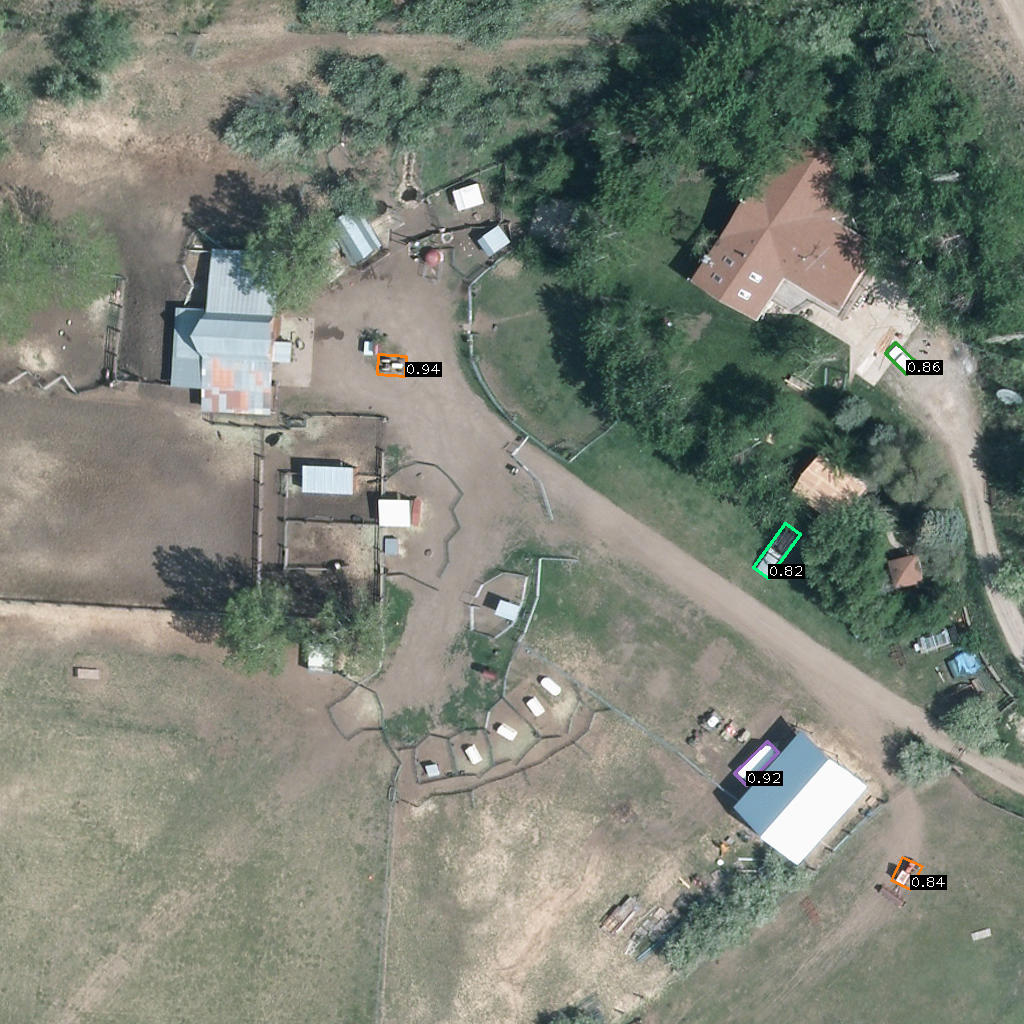
\includegraphics[trim={880pt 630pt 70pt 330pt},clip,width=\linewidth]{images/015Results/01abb_vs_obb/comp_images/obb/523.png}
    %Truck
    & 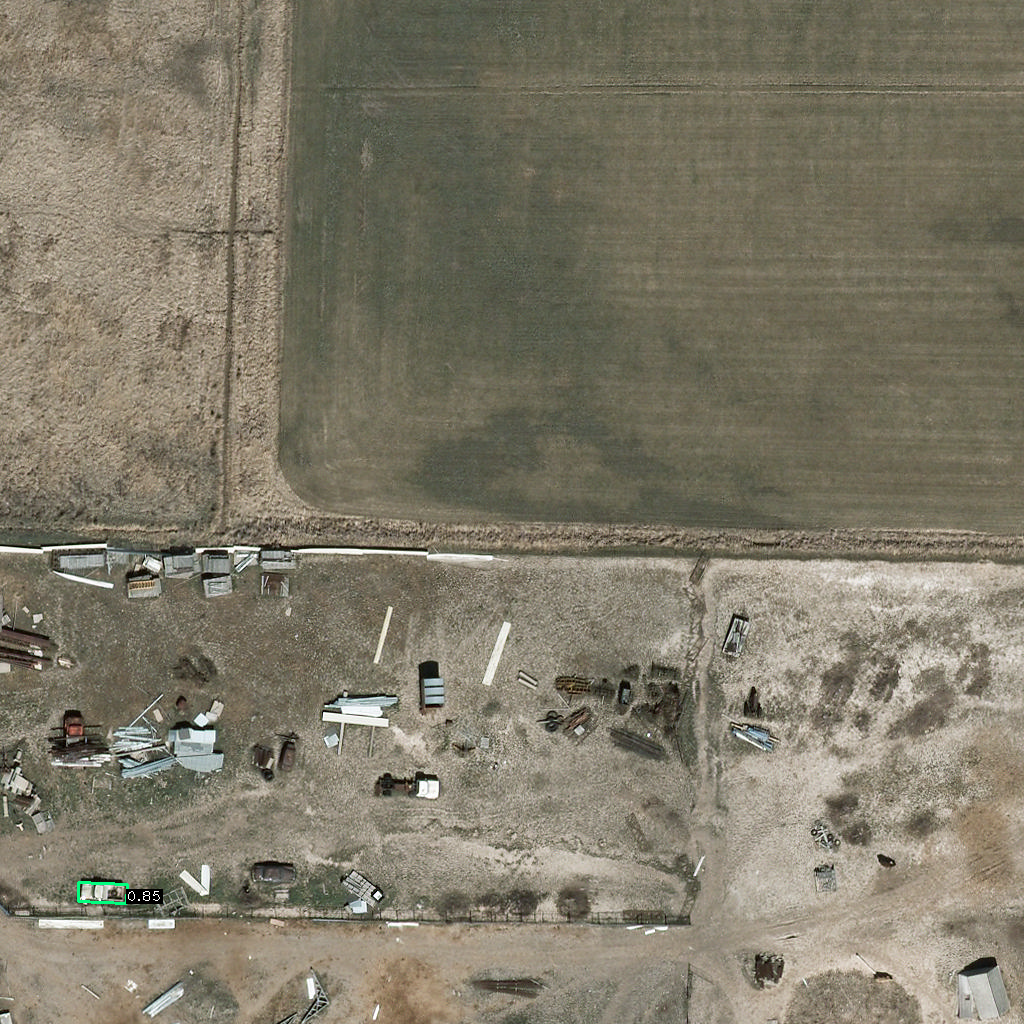
\includegraphics[trim={360pt 200pt 540pt 715pt},clip,width=\linewidth]{images/015Results/01abb_vs_obb/comp_images/obb/212.png}
    %Camping Car
    & 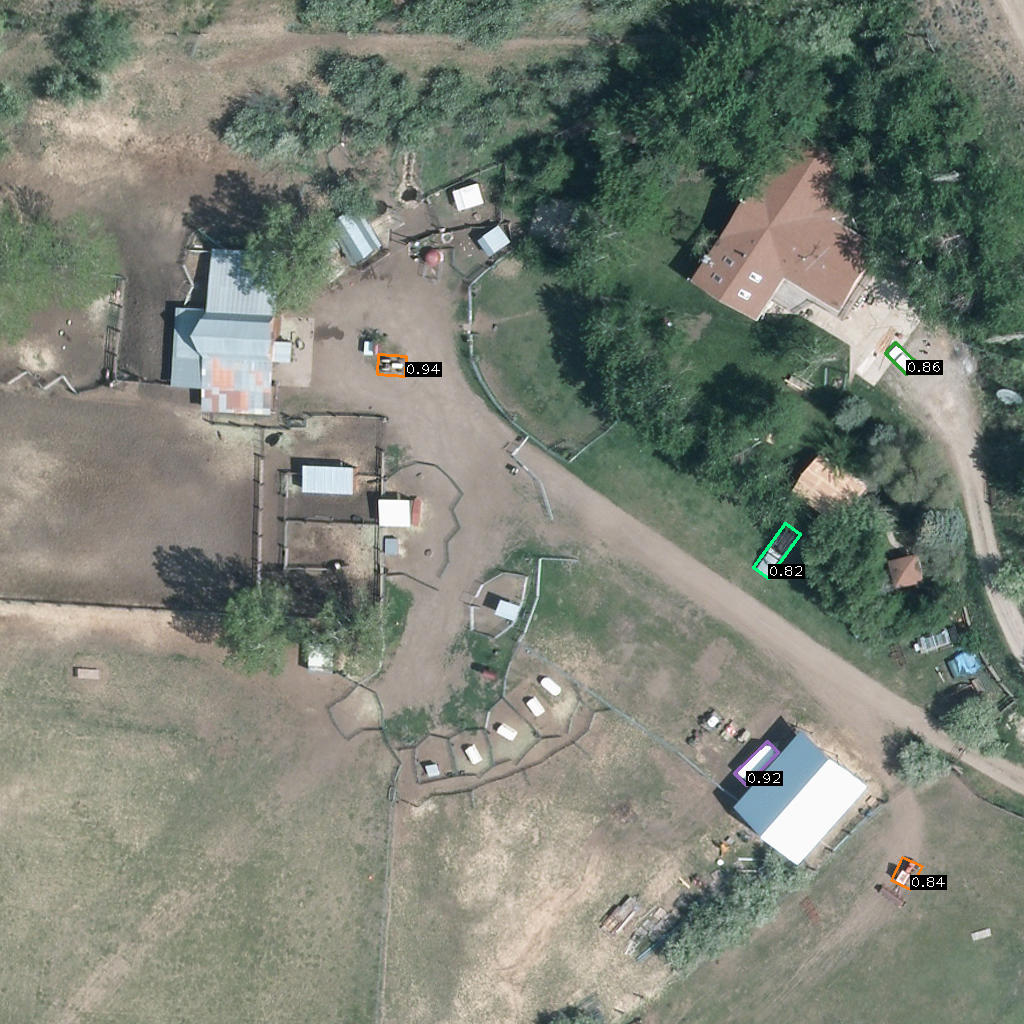
\includegraphics[trim={730pt 220pt 200pt 720pt},clip,width=\linewidth]{images/015Results/01abb_vs_obb/comp_images/obb/523.png}
    %Tractor
    & 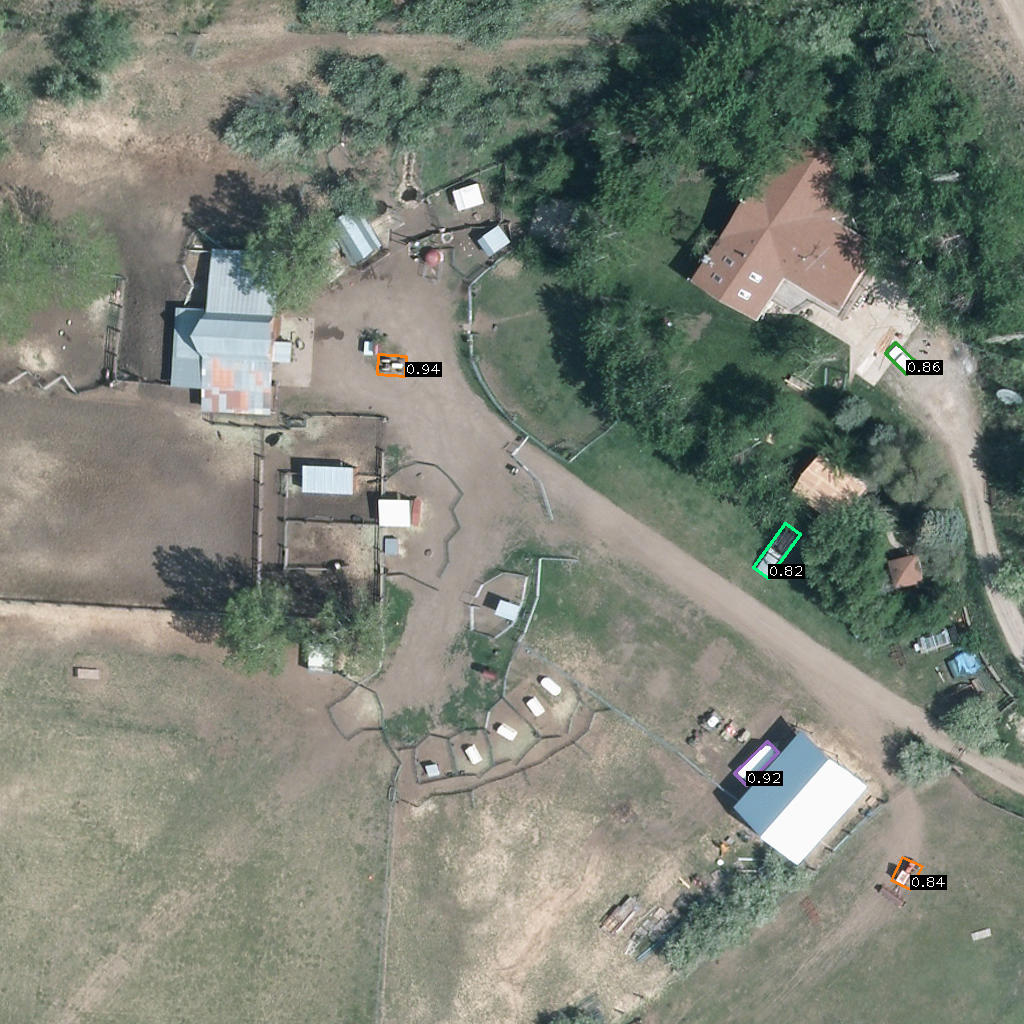
\includegraphics[trim={850pt 110pt 80pt 830pt},clip,width=\linewidth]{images/015Results/01abb_vs_obb/comp_images/obb/523.png}
    %Plane
    &  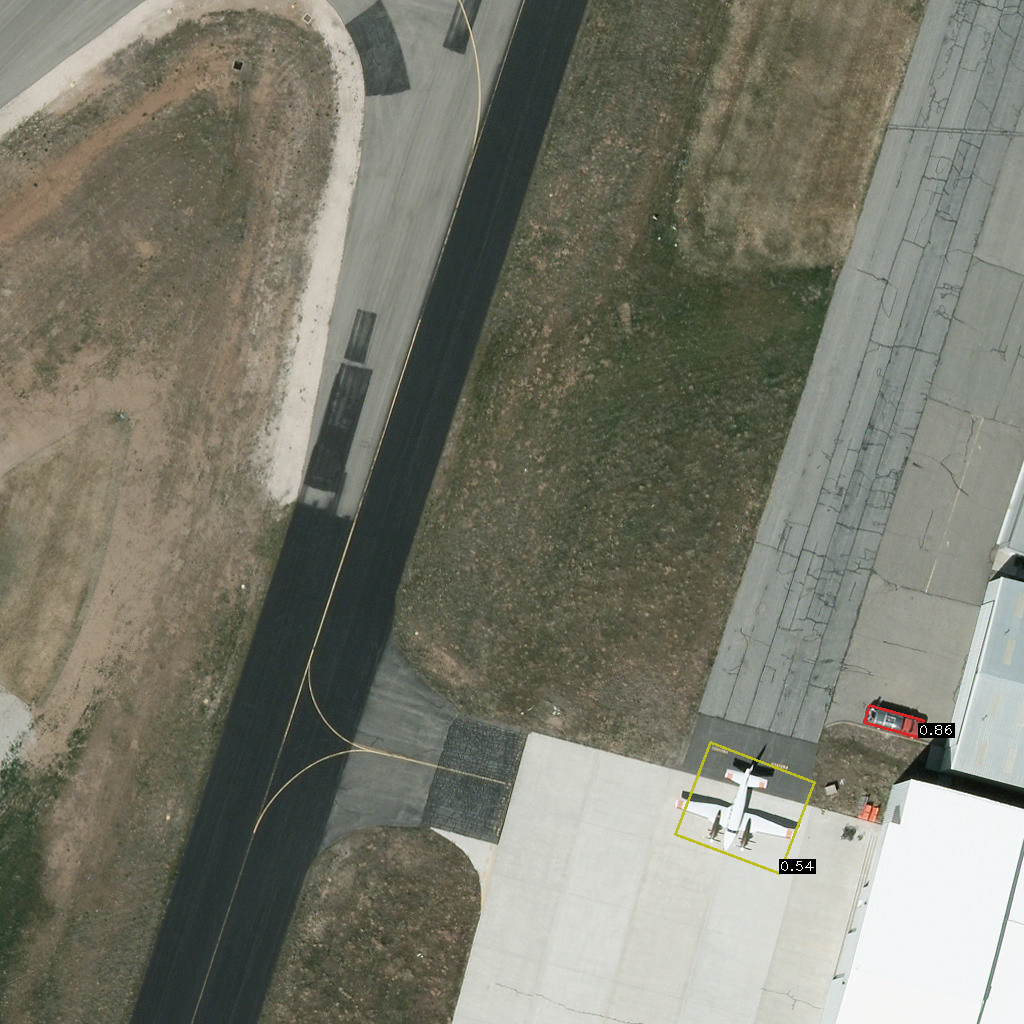
\includegraphics[trim={650pt 120pt 170pt 720pt},clip,width=\linewidth]{images/015Results/01abb_vs_obb/comp_images/obb/487.png}
    %Ship
    & 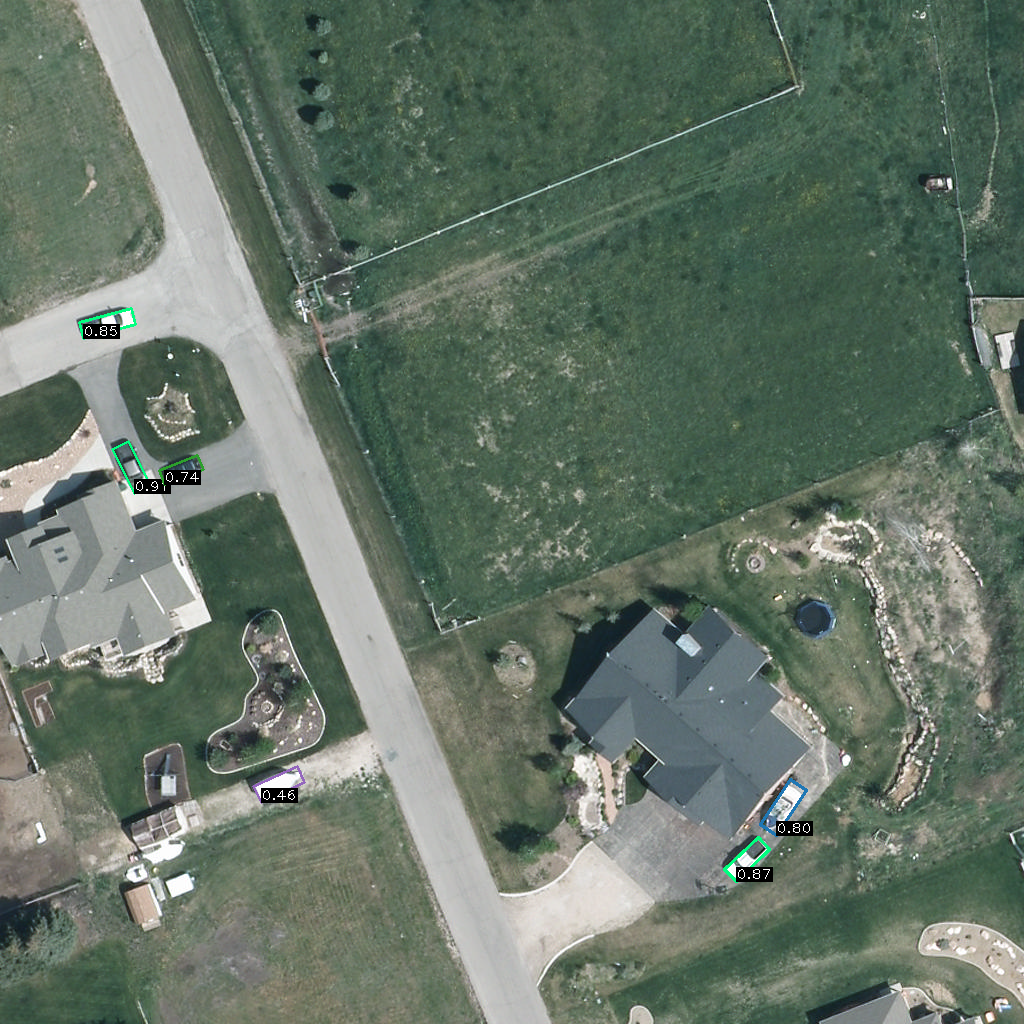
\includegraphics[trim={230pt 200pt 680pt 725pt},clip,width=\linewidth]{images/015Results/01abb_vs_obb/comp_images/obb/509.png}
    %vehicle
    & 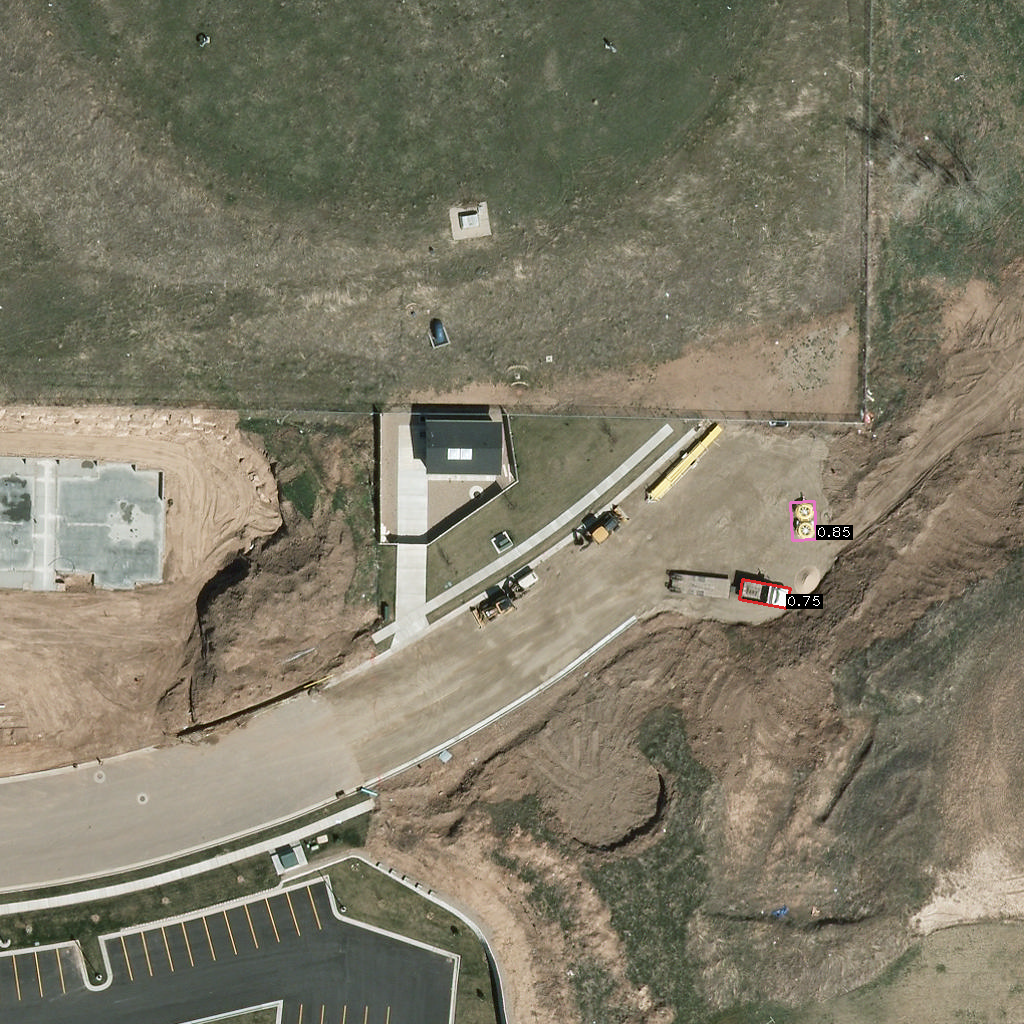
\includegraphics[trim={440pt 360pt 460pt 555pt},clip,width=\linewidth]{images/015Results/01abb_vs_obb/comp_images/obb/427.png}
    %Pick Up
    & 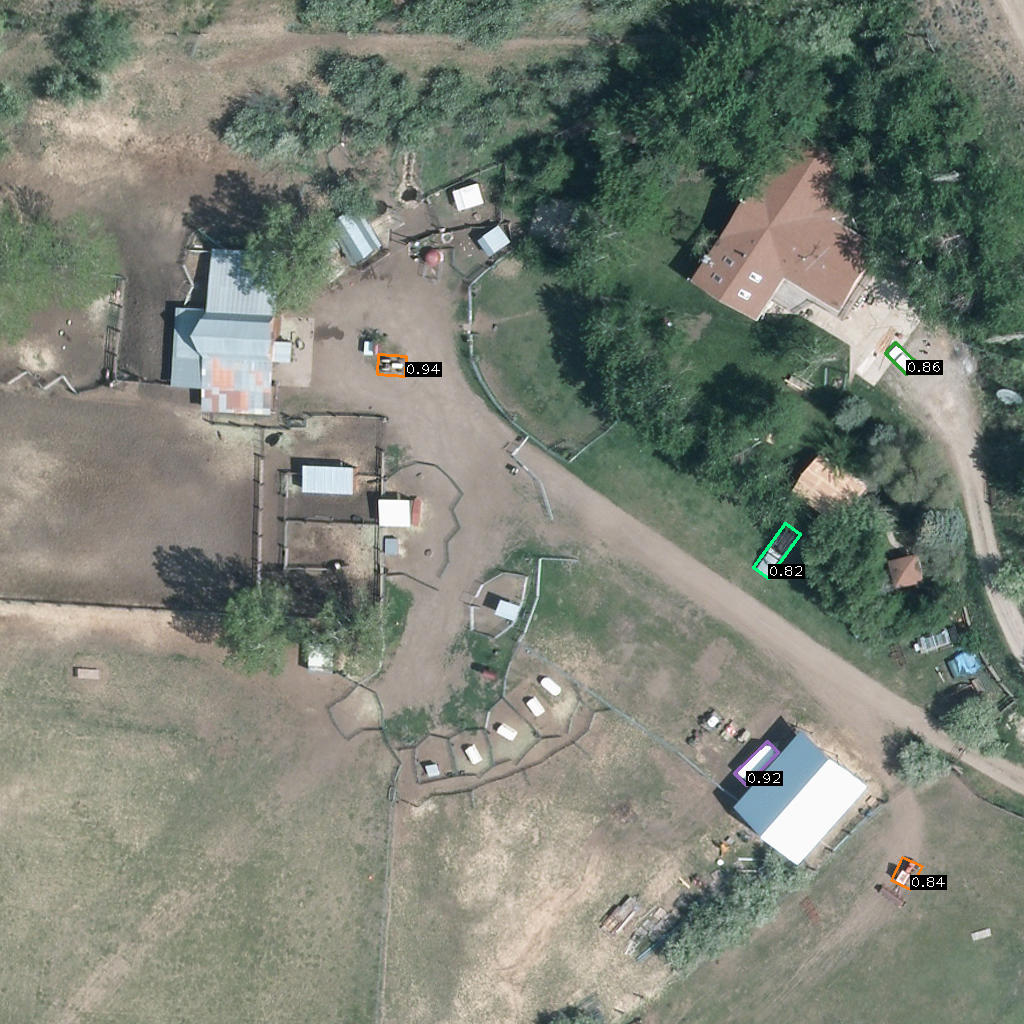
\includegraphics[trim={740pt 420pt 180pt 510pt},clip,width=\linewidth]{images/015Results/01abb_vs_obb/comp_images/obb/523.png}
    %Van
    & 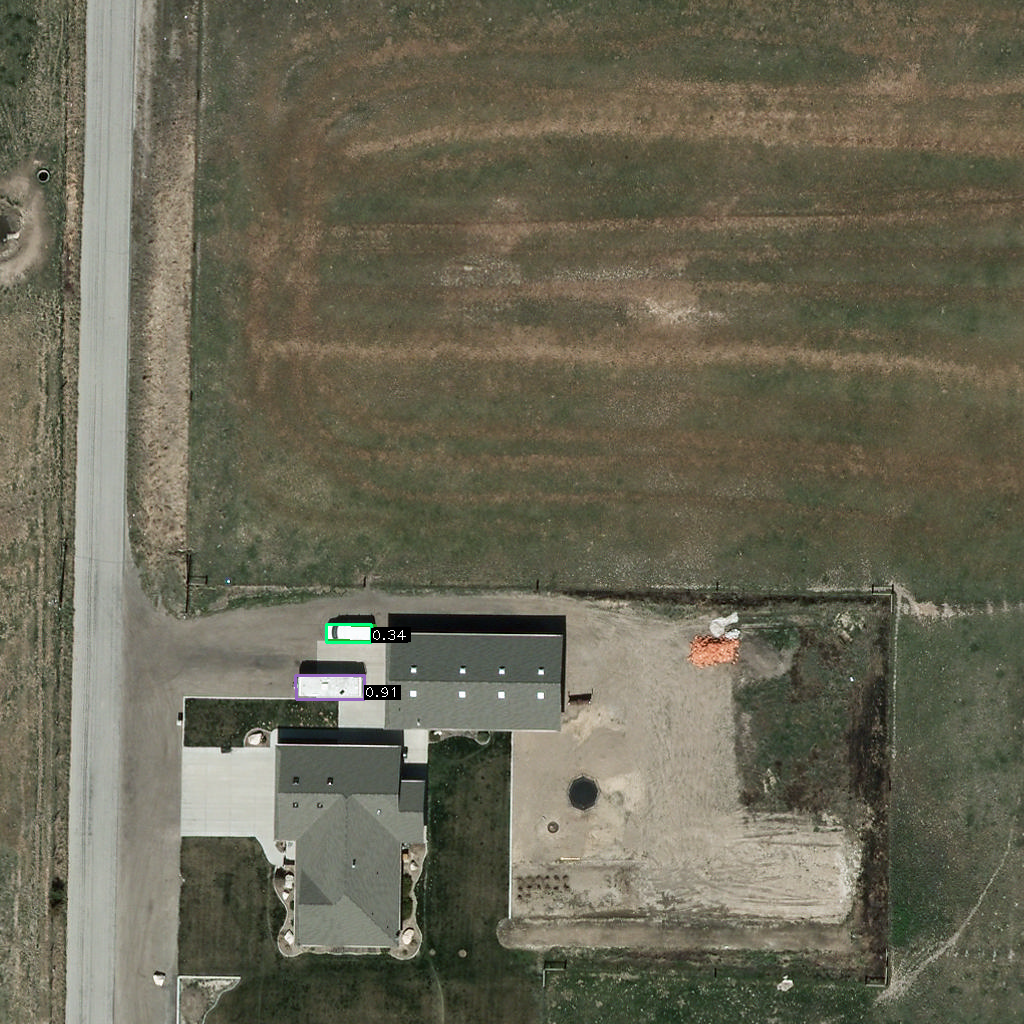
\includegraphics[trim={300pt 355pt 610pt 570pt},clip,width=\linewidth]{images/015Results/01abb_vs_obb/comp_images/obb/198.png} \\ \hline
     \rotatebox{90}{\textbf{\acrshort{abb} in \acrshort{obb}}} 
    %Car
    & 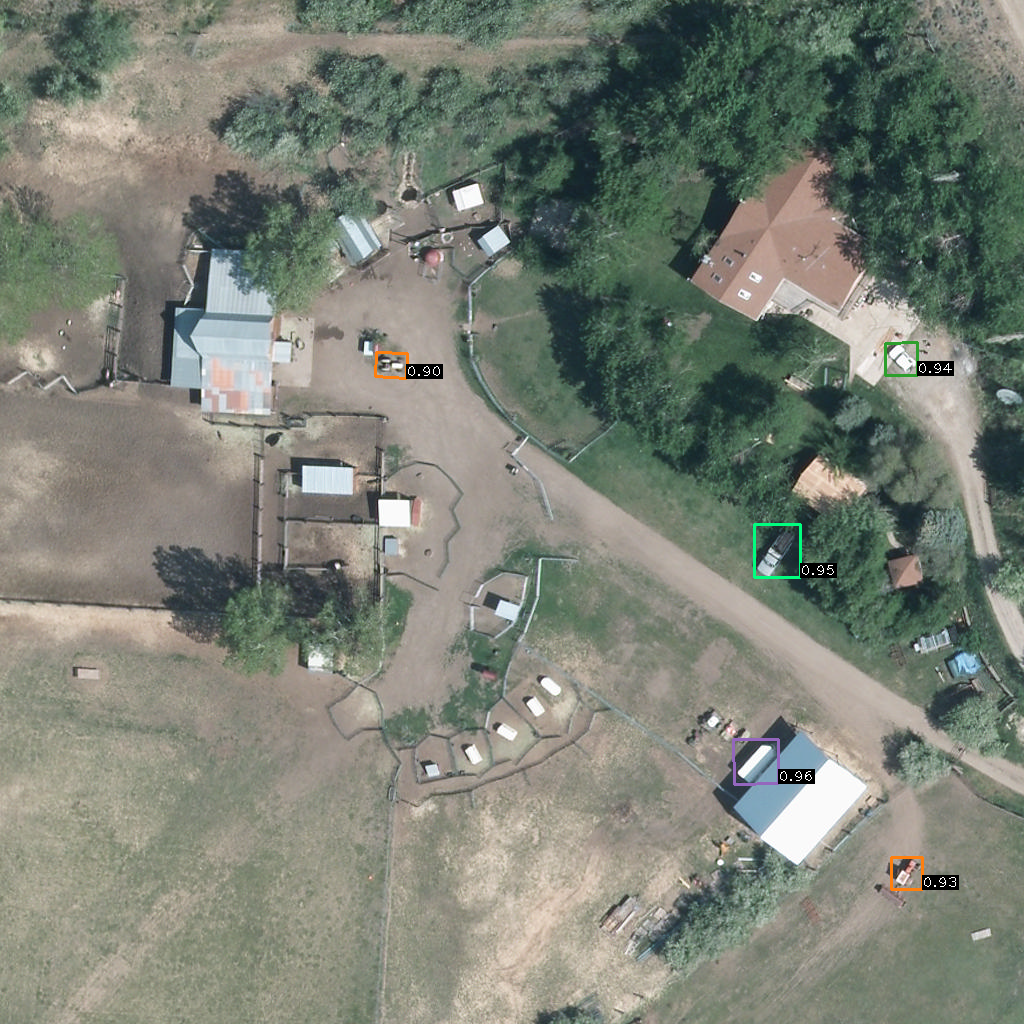
\includegraphics[trim={880pt 630pt 70pt 330pt},clip,width=\linewidth]{images/015Results/01abb_vs_obb/comp_images/aab_old/523.png}
    %Truck
    & 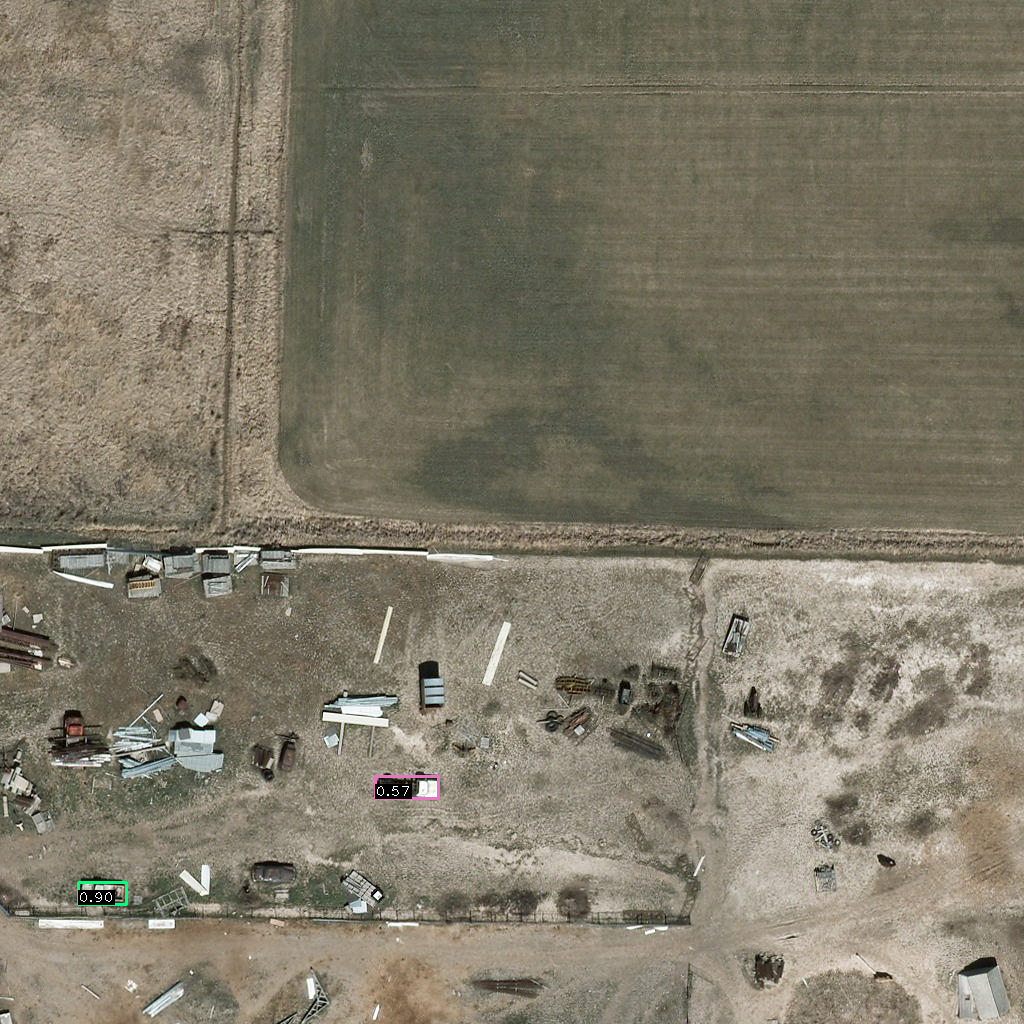
\includegraphics[trim={360pt 200pt 540pt 715pt},clip,width=\linewidth]{images/015Results/01abb_vs_obb/comp_images/aab_old/212.png}
    %Camping Car
    & 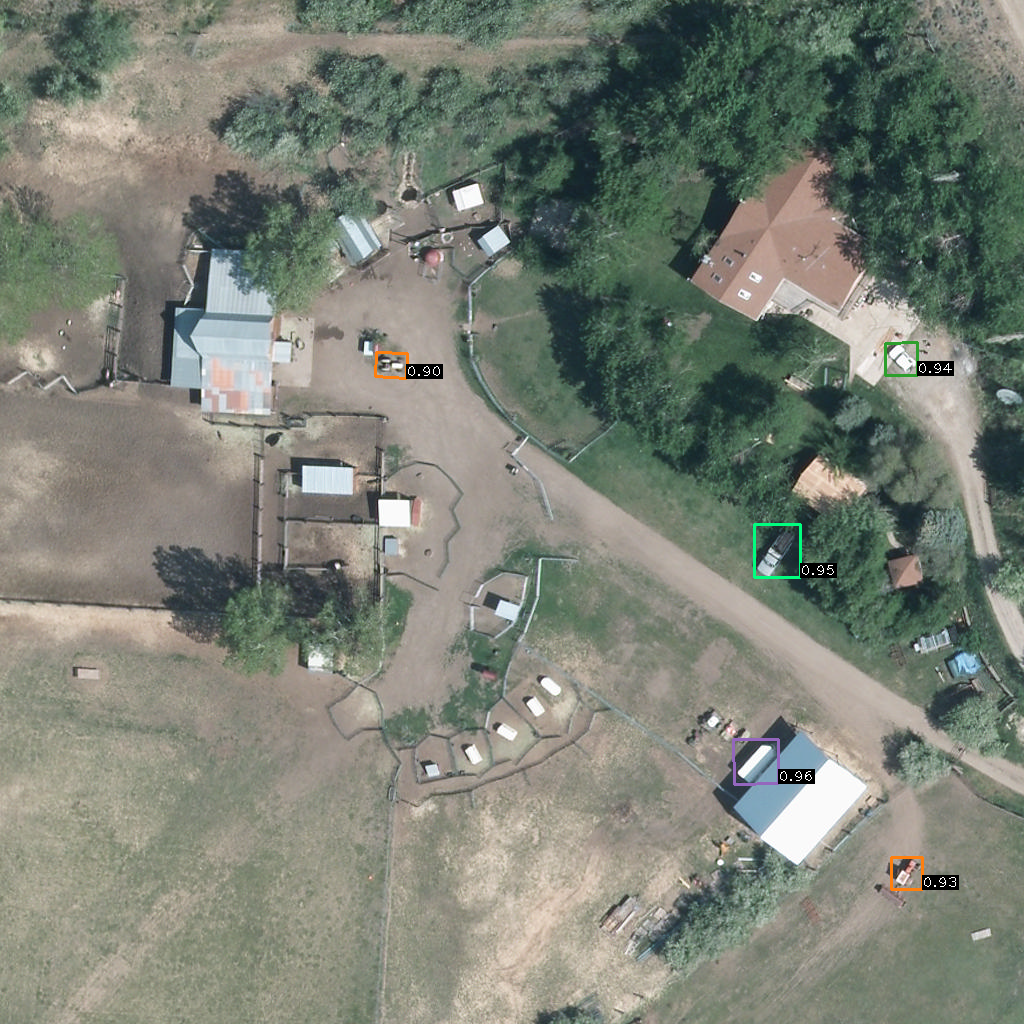
\includegraphics[trim={730pt 220pt 200pt 720pt},clip,width=\linewidth]{images/015Results/01abb_vs_obb/comp_images/aab_old/523.png}
    %Tractor
    & \includegraphics[trim={850pt 110pt 80pt 830pt},clip,width=\linewidth]{images/015Results/01abb_vs_obb/comp_images/aab_old/523.png}
    %Plane
    &  \includegraphics[trim={650pt 120pt 170pt 720pt},clip,width=\linewidth]{images/015Results/01abb_vs_obb/comp_images/aab_old/487.png}
    %Ship
    & \includegraphics[trim={230pt 200pt 680pt 725pt},clip,width=\linewidth]{images/015Results/01abb_vs_obb/comp_images/aab_old/509.png}
    %vehicle
    & \includegraphics[trim={440pt 360pt 460pt 555pt},clip,width=\linewidth]{images/015Results/01abb_vs_obb/comp_images/aab_old/427.png}
    %Pick Up
    & \includegraphics[trim={740pt 420pt 180pt 510pt},clip,width=\linewidth]{images/015Results/01abb_vs_obb/comp_images/aab_old/523.png}
    %Van
    & \includegraphics[trim={300pt 355pt 610pt 570pt},clip,width=\linewidth]{images/015Results/01abb_vs_obb/comp_images/aab_old/198.png} \\ \hline
\end{tabularx}
\caption[aab and obb: Examples of different classes for the object recognition performance]{Examples of different classes for the object recognition performance of different bounding box formats. The numbers displayed on the bounding boxes indicate the confidence of the model in the classification of the respective box. For Color Scheme explanation see Tab. \ref{tab:class_colors}}.
\label{fig:aab_obb_example_pics}
\end{figure}

%##########################################################################
%##########################################################################






\FloatBarrier
%##########################################################################
%##########################################################################
%##########################################################################
%##########################################################################
%##########################################################################
%##########################################################################
%##########################################################################
%##########################################################################
%##########################################################################

\section{Permutation Experiments}
\begin{figure}[t]
    \centering
    \includesvg[width=0.9\textwidth]{images/015Results/02perm_exp/perm_exp_best_val_on_test.svg}
    \caption[Comparison of \acrshort{mAP}@0.5--0.95 values for different channel permutation models (Best validation model on test dataset)]{Comparison of \acrshort{mAP}@0.5--0.95 values for different channel permutation models (Best validation model on test dataset). The red dot is the fold, that has the best \acrshort{mAP}@0.5--0.95 at the validation dataset (see fig. \ref{fig:perm_exp_map50-95:val_on_val}). \acrshort{RGIR} performs best, with models using \acrshort{NDVI} performing significantly worse than the five main permutations. \acrshort{NDVI} may introduce noise. Fluctuations between the quantiles in the main permutations are due to the fact that the channel changes do have an influence. \acrshort{RGBIR} has the third-best performance because it contains all bands. \acrshort{RGB} and \acrshort{RIRB} are better, possibly because too much information also causes noise (Own representation).}
    \label{fig:perm_exp_map50-95:val_on_test}
\end{figure}

\begin{figure}[b]
    \centering
    \includesvg[width=0.9\textwidth]{images/015Results/02perm_exp/perm_exp_best_val_on_val.svg}
    \caption[Comparison of \acrshort{mAP}@0.5--0.95 values for different channel permutation models (Best validation model on validation dataset)]{Comparison of \acrshort{mAP}@0.5--0.95 values for different channel permutation models (Best validation model on validation dataset). The RGBIR channel permutation achieves the best performance, followed by the other main permutations, while RGIR performs worst among the five main permutations. Models with NDVI are again significantly worse due to additional noise. The small fluctuations between the five main quantiles indicate robust folds and stable training (Own representation).}
    \label{fig:perm_exp_map50-95:val_on_val}
\end{figure}
The following section first describes the general results of the models in terms of detection performance and compares them with the \acrshort{mAP}@0.5--0.95 values shown in Figure \ref{fig:perm_exp_map50-95:val_on_test}. This is followed by a detailed analysis of class recognition performance using the difference matrices.  

Figure \ref{fig:perm_exp_map50-95:val_on_test} shows that the RGIR model achieves the best \acrshort{mAP}@0.5--0.95 performance on the test fold, followed by the RIRB and RGB models. The comparatively large differences between the quantiles are striking, indicating a greater dispersion of the results. The RGBIR model ranks fourth, while the IRGB model performs significantly weaker than the aforementioned models, but still achieves better results than the two models that include an NDVI channel. The latter show the weakest overall performance, suggesting that the NDVI channel is of limited use for this task. \todo{is actually analysis} 

Comparing the results with those on the validation dataset (see Figure \ref{fig:perm_exp_map50-95:val_on_val}), there are greater fluctuations between the quantiles overall. While the results of most models are close together in the validation data set and only the NDVI-based models show clear weaknesses, the results in the test data set show a wider range. RGIR in particular shows the largest quantile range here and achieves the weakest robustness compared to the five main models.
 
Table \ref{tab:best_map_fold_perm_exp} summarises the folds per highest \acrshort{mAP} value and model. It is striking in Fig. \ref{fig:perm_exp_map50-95:val_on_test} that most of the red dots are in the median range of the models and only the \acrshort{RGIR} model shows a match between the best fold in the test data set and the best fold in the validation data set.  While each fold performed once or twice as the best validation model on the validation dataset, only fold 2 and fold 3 were able to achieve the top position of the best validation model on the test dataset. This suggests that the generalisation ability of the models can vary greatly and, in particular, that the transferability from the validation to the test dataset is not consistent in all cases.  \todo{is actually analysis}

A more detailed look at the class recognition performance is evident in the difference matrices (see Figure \ref{fig:perm_exp_diffM_all}). These illustrate the specific strengths and weaknesses of the individual models in comparison to RGBIR. While some models show clear advantages for certain classes, systematic misclassifications are evident for other classes. Differences of over 20\% can occur for individual class examples, which significantly influence the overall evaluation of individual models.
  






\begin{table}[h!]
\centering

\begin{tabular}{lcc}
\hline
\textbf{Model} & \textbf{Best mAP Fold (Validation)} & \textbf{Best mAP Fold (Test)} \\ \hline
RGBIR    & 0 & 2 \\
RGB      & 0 & 2 \\
IRGB     & 1 & 3 \\
RIRB     & 4 & 2 \\
RGIR     & 3 & 3 \\
GBNDVI   & 1 & 2 \\
RGBNDVI  & 4 & 2 \\ \hline
\end{tabular}
\caption{Best mAP folds for validation and test sets}
\label{tab:best_map_fold_perm_exp}
\end{table}




\FloatBarrier
\subsection{Comparison with Confusion Matrices}
\label{subsec:permexp_comp_confusion_matric}


\begin{figure}[htbp]
    \centering
    \includesvg[width=0.9\textwidth]{images/015Results/02perm_exp/confusion_matrices/rgbir_F2.svg}
    \caption[Confusion Matrix for RGBIR Modell (Fold 2)]{Confusion Matrix for RGBIR Modell (Fold 2). All values falling within the interval [–0.05, 0.05] are excluded from the matrix. The model performs very well on the training data. The class \textit{Plane} is perfectly recognised and classified, while \textit{Car}, \textit{Ship} and \textit{Tractor} achieve excellent results. The generic class \textit{Vehicle} is often confused with the background, presumably due to the high variability of the object types it contains and because it is generic, meaning that there are no clear shapes and colours. The good recognition rate for \textit{Car} illustrates the strong influence of a large amount of training data on classification accuracy (Own representation).}
    \label{fig:perm_exp_confM_rgbir_f2}
\end{figure}

The confusion matrix for the RGBIR model (Fold 2) shown in Figure~\ref{fig:perm_exp_confM_rgbir_f2} demonstrates very strong performance. In particular, the model achieves a perfect recognition rate of 100\% for the \textit{Plane} class. The classes \textit{Car}, \textit{Ship}, and \textit{Tractor} also show excellent performance of over 80\%. Good results in the range of 60–80\% are achieved for the classes \textit{Truck}, \textit{Camping Car}, \textit{Van}, and \textit{Pick Up}. The generic class \textit{Vehicle} shows an acceptable recognition rate of over 52\%. However, the problem is that the class \textit{Vehicle} is often misclassified as \textit{Background} (over 40\%). In addition, there is an increased misclassification rate for \textit{Camping Car} (28~\%) and \textit{Truck} (16~\%), while the remaining classes range between 8–12~\%. Due to this strong overall performance, the RGBIR model (Fold~2) serves as the basis for the difference matrices. Another decisive factor is that all available bands are included unchanged in raw form in this permutation run.

Difference matrices are generated for the quantitative analysis of the differences between the predictions of different models. The confusion matrices are first normalised row by row and then subtracted from each other element by element. Minor deviations within the range of -0.05-0.05\% are masked and not displayed so as not to overestimate them. Due to the partially inferior label representation, the extent of which cannot be quantified and which is briefly explained in the following paragraph, the differences in the last column (background/object distinction) are only taken into account to a limited extent in the following analysis.

Fig. \ref{fig:wrong_labels} shows that the quality of the label annotation is sometimes inadequate. For example, image 34, which depicts a typical suburban environment, contains no annotated objects, even though vehicles are clearly visible. However, the trained model recognises them with high confidence. As a result, the selectivity between \acrshort{GT} background and objects is impaired, which is particularly reflected in the last column of the confusion matrix.

The following applies to the interpretation of the difference matrices: Red indicates better performance of the RGBIR (F2) model, blue indicates better performance of the comparison model. The stronger the colour intensity, the greater the difference. The differences are divided into four categories: low (0–5\%), moderate (5–10\%), high (10–20\%) and very high (>20\%) (see Table~\ref{tab:diff_cat}). The comparison sequence starts with the weakest model and progresses to the best model according to the results in Figure~\ref{fig:perm_exp_map50-95:val_on_test}.



\begin{figure}[h] 
    \centering
    % Erste Subfigur
    \begin{subfigure}[b]{0.45\textwidth} % [b] für bottom alignment, 0.48\textwidth damit noch Platz ist
        \includegraphics[width=\textwidth]{images/015Results/wrong_labels/comp_images/00000034_co.png} % Bildpfad zum ersten Bild
        \caption{\Acrlong{GT} } % Unterschrift für das erste Bild
        \label{fig:cm_trgbir} % Label für Referenzierung von Bild 1
    \end{subfigure}
    \hfill % Fügt horizontalen Platz zwischen den Subfiguren ein
    % Zweite Subfigur
    \begin{subfigure}[b]{0.45\textwidth} % 0.48\textwidth für das zweite Bild
        \includegraphics[width=\textwidth]{images/015Results/wrong_labels/comp_images/rgbir/34.png} % Bildpfad zum zweiten Bild
        \caption{Prediction} % Unterschrift für das zweite Bild
        \label{fig:cm_irgb} % Label für Referenzierung von Bild 2
    \end{subfigure}
    \caption[Comparison \acrshort{GT} and Prediction (RGBIR, F0, Validation on Validation Dataset) of image 00000034\_co.png]{Comparison of image 00000034\_co.png shows a discrepancy between ground truth and model prediction: vehicles are recognisable in the GT but not annotated, while the model (RGBIR, F0, (Validation on Validation)) detects and classifies them correctly. This calls into question the validity of GT-based metrics for distinguishing between background and object (Own representation).} % Gemeinsame Unterschrift für beide Bilder
    \label{fig:wrong_labels} % Label für die gesamte Figure-Umgebung
\end{figure}


\begin{table}[h]
\centering
\begin{tabular}{c c}
\hline
\textbf{Difference (in \% from reference)} & \textbf{Category} \\ \hline
0 -- 5 \%   & low \\ 
5 -- 10 \%  & moderate \\ 
10 -- 20 \% & high \\ 
> 20 \%     & very high \\ \hline
\end{tabular}
\caption{Classification of differences relative to the reference}
\label{tab:diff_cat}
\end{table}

\begin{figure}[htbp]
    \centering
    % Erste Spalte
    \begin{subfigure}{0.48\textwidth}
        \centering
        \includesvg[width=\linewidth]{images/015Results/02perm_exp/confusion_matrices/Difference_Matrices/RGBIR_F2_vs_RGBNDVI_F2.svg}
        \caption{RGBNDVI (F2)}
        \label{fig:perm_exp_diffM_rgbndvi_f2}
    \end{subfigure}
    \begin{subfigure}{0.48\textwidth}
        \centering
        \includesvg[width=\linewidth]{images/015Results/02perm_exp/confusion_matrices/Difference_Matrices/RGBIR_F2_vs_GBNDVI_F2.svg}
        \caption{GBNDVI (F2)}
        \label{fig:perm_exp_diffM_gbndvi_f2}
    \end{subfigure}
    
    \begin{subfigure}{0.48\textwidth}
        \centering
        \includesvg[width=\linewidth]{images/015Results/02perm_exp/confusion_matrices/Difference_Matrices/RGBIR_F2_vs_IRGB_F3.svg}
        \caption{IRGB (F3)}
        \label{fig:perm_exp_diffM_irgb_f3}
    \end{subfigure}
    \begin{subfigure}{0.48\textwidth}
        \centering
        \includesvg[width=\linewidth]{images/015Results/02perm_exp/confusion_matrices/Difference_Matrices/RGBIR_F2_vs_RIRB_F2.svg}
        \caption{RIRB (F2)}
        \label{fig:perm_exp_diffM_RIRB_f2}
    \end{subfigure}
    
    \begin{subfigure}{0.48\textwidth}
        \centering
        \includesvg[width=\linewidth]{images/015Results/02perm_exp/confusion_matrices/Difference_Matrices/RGBIR_F2_vs_RGB_F2.svg}
        \caption{RGB (F2)}
        \label{fig:perm_exp_diffM_RGB_f2}
    \end{subfigure}
    \begin{subfigure}{0.48\textwidth}
        \centering
        \includesvg[width=\linewidth]{images/015Results/02perm_exp/confusion_matrices/Difference_Matrices/RGBIR_F2_vs_RGIR_F3.svg}
        \caption{RGIR (F3)}
        \label{fig:perm_exp_diffM_RGIR_f3}
    \end{subfigure}

    \caption[Difference Matrices compared to RGBIR (Fold 2)]{Difference Matrices for all models compared against RGBIR (Fold 2). Red indicates better performance for RGBIR, blue for the respective comparison model. All values falling within the interval [–0.05, 0.05] are excluded from the matrices. Clear differences exist between channel permutations. \textit{Ship} and \textit{Tractor} are best recognised by RGBIR, while RGIR shows minimal differences. Object-background distinction remains challenging for all models, with RGIR yielding the most stable results (own representation).}
    \label{fig:perm_exp_diffM_all}
\end{figure}
\todo{Beschreibung Figures länger machen, mehr Analyse weniger "was sieht man"}



Figure~\ref{fig:perm_exp_diffM_rgbndvi_f2} illustrates clear differences in favour of RGBIR. This is particularly evident in the correct recognition of \textit{Ship} (+24~\%), \textit{Vehicle} (+16~\%), \textit{Plane} (+12~\%) and \textit{Tractor} (10~\%). There are also differences of more than 10\% in cases of confusion between \textit{Van} and \textit{Car}. In contrast, RGBNDVI has fewer misclassifications, for example in the case of \textit{Plane} (-12\%) and \textit{Van} (-23\%), which are less frequently misidentified as \textit{Background}. Overall, RGBIR shows five classes (\textit{Ship}, \textit{Tractor}, \textit{Vehicle}, \textit{Van}, \textit{Plane}) in which it performs at least 5\% better, while RGBNDVI does not show any higher classification accuracy.


Figure~\ref{fig:perm_exp_diffM_gbndvi_f2} shows a very large difference in the \textit{Tractor} class, where RGBIR is clearly superior (+22\%). In contrast, the improvement for \textit{Ship} is only +8\%. It is striking that \textit{Tractor} (-15\%), \textit{Ship} (-12\%) and \textit{Van} (-11\%) are less frequently misclassified as \textit{Background} in the GBNDVI model. Overall, RGBIR is at least 5\% better in four classes (\textit{Ship}, \textit{Tractor}, \textit{Van}, \textit{Vehicle}), while GBNDVI does not show higher accuracy in any class.




As Figure~\ref{fig:perm_exp_diffM_irgb_f3} shows, \textit{Ship} remains a class in which RGBIR is particularly strong (+21~\%). Nevertheless, misclassifications occur in both models, such as the confusion of \textit{Ship} with \textit{Camping Car} (-14\%) or \textit {Background} (-12\%). Overall, RGBIR is at least 5\% better in three classes (\textit{Ship}, \textit{Camping Car}, \textit{Vehicle}), while IRGB does not show higher accuracy in any class.




Figure~\ref{fig:perm_exp_diffM_RIRB_f2} shows a mixed picture: RGBIR has advantages in distinguishing object/background with the classes vehicle and camping car, while RIRB achieves a moderate improvement in background/object distinction (6\%) for camping cars. Noteworthy are the less frequent misclassifications in the RIRB model, where \textit{Van} (21\%) and \textit{Ship} (12\%) are not recognised as \textit{Background}. Overall, RGBIR is better in two classes (\textit{Ship}, \textit{Van}), while RIRB has higher accuracy in one class (\textit{Camping Car}).




Figure~\ref{fig:perm_exp_diffM_RGB_f2} shows clear differences in favour of the RGBIR model in the classes \textit{Ship} (12~\%) and \textit{Vehicle} (15~\%). Nevertheless, moderate misclassifications also occur here, such as the confusion of \textit{Pick Up} with \textit{Car} (6~\%) or \textit{Van} with \textit{Pick Up} (6~\%). While RGB misclassifies \textit{Vehicle} (15\%) and \textit{Ship} (10\%) less frequently than \textit{Background}, RGBIR more frequently misclassifies \textit{Background} as \textit{Pick Up} (7\%). Overall, RGBIR is superior in two classes (\textit{Ship}, \textit{Vehicle}).



The last comparison in Figure~\ref{fig:perm_exp_diffM_RGIR_f3} between RGBIR and RGIR (Fold~3) shows an almost equal result. While RGBIR confuses \textit{Van} with \textit{Car} more often (12\%) and classifies \textit{Camping Car} more often than \textit{Background} (10\%), RGIR performs moderately better for \textit{Ship} (6\%) and \textit{Van} (8\%). Overall, both models show comparable performance, with neither achieving higher classification accuracy for any one class.

Figure \ref{fig:perm_exp_example_pics} illustrates the recognition performance of the different models for the classes present in the \acrshort{VEDAI} dataset. The outstanding classification performance of all models for the \textit{Car} class is particularly evident. The situation is similar for the \textit{Truck} class, although in the example shown, the IRGB model sometimes classifies the objects as both \textit{Truck} and \textit{Vehicle}. The models also show very good results for the classes \textit{Camping Car}, \textit{Tractor}, \textit{Plane}, \textit{Pick Up} and \textit{Van}, although the GBNDVI model confuses \textit{Van} with \textit{Car}, albeit with low confidence. The class \textit{Ship} is misclassified by almost all models as \textit{Camping Car} with low confidence; RGBIR and IRGB also double-classify it as \textit{Ship} and \textit{Camping Car}. Only the RGBNDVI model correctly recognises \textit{Ship}. It is striking that the class \textit{Vehicle} is not reliably recognised by any of the models.


\begin{figure}[h!]
\centering
\renewcommand{\arraystretch}{1.2} % mehr Platz zwischen Zeilen
\setlength{\tabcolsep}{2pt} % weniger Platz zwischen Spalten
\begin{tabularx}{\textwidth}{c|*{9}{X}}
    & \textbf{Car}
    & \textbf{Truck}
    & \textbf{Camping Car}
    & \textbf{Tractor}
    & \textbf{Plane}
    & \textbf{Ship}
    & \textbf{Vehicle}
    & \textbf{Pick-Up}
    & \textbf{Van} \\ \hline
    \rotatebox{90}{\textbf{\acrshort{GT} (\acrshort{abb})}} 
    %Car
    & \includegraphics[trim={880pt 630pt 70pt 330pt},clip,width=\linewidth]{images/015Results/01abb_vs_obb/comp_images/ground_truth_abb/523.png}
    %Truck
    & \includegraphics[trim={360pt 200pt 540pt 715pt},clip,width=\linewidth]{images/015Results/01abb_vs_obb/comp_images/ground_truth_abb/212.png}
    %Camping Car
    & \includegraphics[trim={730pt 220pt 200pt 720pt},clip,width=\linewidth]{images/015Results/01abb_vs_obb/comp_images/ground_truth_abb/523.png}
    %Tractor
    & \includegraphics[trim={850pt 110pt 80pt 830pt},clip,width=\linewidth]{images/015Results/01abb_vs_obb/comp_images/ground_truth_abb/523.png}
    %Plane
    &  \includegraphics[trim={650pt 120pt 170pt 720pt},clip,width=\linewidth]{images/015Results/01abb_vs_obb/comp_images/ground_truth_abb/487.png}
    %Ship
    & \includegraphics[trim={230pt 200pt 680pt 725pt},clip,width=\linewidth]{images/015Results/01abb_vs_obb/comp_images/ground_truth_abb/509.png}
    %vehicle
    & \includegraphics[trim={440pt 360pt 460pt 555pt},clip,width=\linewidth]{images/015Results/01abb_vs_obb/comp_images/ground_truth_abb/427.png}
    %Pick Up
    & \includegraphics[trim={740pt 420pt 180pt 510pt},clip,width=\linewidth]{images/015Results/01abb_vs_obb/comp_images/ground_truth_abb/523.png}
    %Van
    & \includegraphics[trim={300pt 355pt 610pt 570pt},clip,width=\linewidth]{images/015Results/01abb_vs_obb/comp_images/ground_truth_abb/198.png} \\ \hline

    \rotatebox{90}{\textbf{\acrshort{GT} (\acrshort{obb})}} 
    %Car
    & \includegraphics[trim={880pt 630pt 70pt 330pt},clip,width=\linewidth]{images/015Results/01abb_vs_obb/comp_images/ground_truth_obb/523.png}
    %Truck
    & \includegraphics[trim={360pt 200pt 540pt 715pt},clip,width=\linewidth]{images/015Results/01abb_vs_obb/comp_images/ground_truth_obb/212.png}
    %Camping Car
    & \includegraphics[trim={730pt 220pt 200pt 720pt},clip,width=\linewidth]{images/015Results/01abb_vs_obb/comp_images/ground_truth_obb/523.png}
    %Tractor
    & \includegraphics[trim={850pt 110pt 80pt 830pt},clip,width=\linewidth]{images/015Results/01abb_vs_obb/comp_images/ground_truth_obb/523.png}
    %Plane
    &  \includegraphics[trim={650pt 120pt 170pt 720pt},clip,width=\linewidth]{images/015Results/01abb_vs_obb/comp_images/ground_truth_obb/487.png}
    %Ship
    & \includegraphics[trim={230pt 200pt 680pt 725pt},clip,width=\linewidth]{images/015Results/01abb_vs_obb/comp_images/ground_truth_obb/509.png}
    %vehicle
    & \includegraphics[trim={440pt 360pt 460pt 555pt},clip,width=\linewidth]{images/015Results/01abb_vs_obb/comp_images/ground_truth_obb/427.png}
    %Pick Up
    & \includegraphics[trim={740pt 420pt 180pt 510pt},clip,width=\linewidth]{images/015Results/01abb_vs_obb/comp_images/ground_truth_obb/523.png}
    %Van
    & \includegraphics[trim={300pt 355pt 610pt 570pt},clip,width=\linewidth]{images/015Results/01abb_vs_obb/comp_images/ground_truth_obb/198.png} \\ \hline
    \rotatebox{90}{\textbf{\acrshort{abb}}} 
    %Car
    & \includegraphics[trim={880pt 630pt 70pt 330pt},clip,width=\linewidth]{images/015Results/01abb_vs_obb/comp_images/abb/523.png}
    %Truck
    & \includegraphics[trim={360pt 200pt 540pt 715pt},clip,width=\linewidth]{images/015Results/01abb_vs_obb/comp_images/abb/212.png}
    %Camping Car
    & \includegraphics[trim={730pt 220pt 200pt 720pt},clip,width=\linewidth]{images/015Results/01abb_vs_obb/comp_images/abb/523.png}
    %Tractor
    & \includegraphics[trim={850pt 110pt 80pt 830pt},clip,width=\linewidth]{images/015Results/01abb_vs_obb/comp_images/abb/523.png}
    %Plane
    &  \includegraphics[trim={650pt 120pt 170pt 720pt},clip,width=\linewidth]{images/015Results/01abb_vs_obb/comp_images/abb/487.png}
    %Ship
    & \includegraphics[trim={230pt 200pt 680pt 725pt},clip,width=\linewidth]{images/015Results/01abb_vs_obb/comp_images/abb/509.png}
    %vehicle
    & \includegraphics[trim={440pt 360pt 460pt 555pt},clip,width=\linewidth]{images/015Results/01abb_vs_obb/comp_images/abb/427.png}
    %Pick Up
    & \includegraphics[trim={740pt 420pt 180pt 510pt},clip,width=\linewidth]{images/015Results/01abb_vs_obb/comp_images/abb/523.png}
    %Van
    & \includegraphics[trim={300pt 355pt 610pt 570pt},clip,width=\linewidth]{images/015Results/01abb_vs_obb/comp_images/abb/198.png} \\ \hline
    \rotatebox{90}{\textbf{\acrshort{obb}}} 
    %Car
    & \includegraphics[trim={880pt 630pt 70pt 330pt},clip,width=\linewidth]{images/015Results/01abb_vs_obb/comp_images/obb/523.png}
    %Truck
    & \includegraphics[trim={360pt 200pt 540pt 715pt},clip,width=\linewidth]{images/015Results/01abb_vs_obb/comp_images/obb/212.png}
    %Camping Car
    & \includegraphics[trim={730pt 220pt 200pt 720pt},clip,width=\linewidth]{images/015Results/01abb_vs_obb/comp_images/obb/523.png}
    %Tractor
    & \includegraphics[trim={850pt 110pt 80pt 830pt},clip,width=\linewidth]{images/015Results/01abb_vs_obb/comp_images/obb/523.png}
    %Plane
    &  \includegraphics[trim={650pt 120pt 170pt 720pt},clip,width=\linewidth]{images/015Results/01abb_vs_obb/comp_images/obb/487.png}
    %Ship
    & \includegraphics[trim={230pt 200pt 680pt 725pt},clip,width=\linewidth]{images/015Results/01abb_vs_obb/comp_images/obb/509.png}
    %vehicle
    & \includegraphics[trim={440pt 360pt 460pt 555pt},clip,width=\linewidth]{images/015Results/01abb_vs_obb/comp_images/obb/427.png}
    %Pick Up
    & \includegraphics[trim={740pt 420pt 180pt 510pt},clip,width=\linewidth]{images/015Results/01abb_vs_obb/comp_images/obb/523.png}
    %Van
    & \includegraphics[trim={300pt 355pt 610pt 570pt},clip,width=\linewidth]{images/015Results/01abb_vs_obb/comp_images/obb/198.png} \\ \hline
     \rotatebox{90}{\textbf{\acrshort{abb} in \acrshort{obb}}} 
    %Car
    & \includegraphics[trim={880pt 630pt 70pt 330pt},clip,width=\linewidth]{images/015Results/01abb_vs_obb/comp_images/aab_old/523.png}
    %Truck
    & \includegraphics[trim={360pt 200pt 540pt 715pt},clip,width=\linewidth]{images/015Results/01abb_vs_obb/comp_images/aab_old/212.png}
    %Camping Car
    & \includegraphics[trim={730pt 220pt 200pt 720pt},clip,width=\linewidth]{images/015Results/01abb_vs_obb/comp_images/aab_old/523.png}
    %Tractor
    & \includegraphics[trim={850pt 110pt 80pt 830pt},clip,width=\linewidth]{images/015Results/01abb_vs_obb/comp_images/aab_old/523.png}
    %Plane
    &  \includegraphics[trim={650pt 120pt 170pt 720pt},clip,width=\linewidth]{images/015Results/01abb_vs_obb/comp_images/aab_old/487.png}
    %Ship
    & \includegraphics[trim={230pt 200pt 680pt 725pt},clip,width=\linewidth]{images/015Results/01abb_vs_obb/comp_images/aab_old/509.png}
    %vehicle
    & \includegraphics[trim={440pt 360pt 460pt 555pt},clip,width=\linewidth]{images/015Results/01abb_vs_obb/comp_images/aab_old/427.png}
    %Pick Up
    & \includegraphics[trim={740pt 420pt 180pt 510pt},clip,width=\linewidth]{images/015Results/01abb_vs_obb/comp_images/aab_old/523.png}
    %Van
    & \includegraphics[trim={300pt 355pt 610pt 570pt},clip,width=\linewidth]{images/015Results/01abb_vs_obb/comp_images/aab_old/198.png} \\ \hline
\end{tabularx}
\caption[aab and obb: Examples of different classes for the object recognition performance]{Examples of different classes for the object recognition performance of different bounding box formats. The numbers displayed on the bounding boxes indicate the confidence of the model in the classification of the respective box. For Color Scheme explanation see Tab. \ref{tab:class_colors}}.
\label{fig:aab_obb_example_pics}
\end{figure}
\FloatBarrier






%##########################################################################
%##########################################################################
%##########################################################################
%##########################################################################
%##########################################################################
%##########################################################################
%##########################################################################
%##########################################################################
%##########################################################################
\section{Ablation Studies}

The box plots in Fig. \ref{fig:ablation_map50-95:val_on_test} of the 6-fold cross-validation show that the models for the red, green, blue and IR channels are in the range of \acrshort{mAP}@0.5--0.95 = 0.52–0.54 on the test data set. A single value in the IR model reaches 0.5777, but this is well outside the central range of the other folds and should be interpreted as an outlier. Overall, no significant differences can be observed between the Red, Green, Blue and IR models, while NDVI performs significantly worse with a median of around 0.44. Similar results can be seen in Fig. \ref{fig:ablation_map50-95:val_on_val} for the performance on the validation data.

The evaluation of the results in Tab. \ref{tab:ablation_best_folds_test} also shows that fold 4 and fold 2 in particular achieved the best results on the validation data set. On the test data set, however, folds 0, 2 and 3 achieve the best performance.  

Overall, the IR model shows the highest performance and achieves the highest \acrshort{mAP} value compared to the other variants examined.




\begin{figure}[htbp]
    \centering
    \includesvg[width=0.8\textwidth]{images/015Results/03ablation/best_val_on_test.svg}
    \caption[Comparison of \acrshort{mAP}@0.5--0.95 values for channels: red, green, blue, ndvi (Best validation model on test dataset)]{Comparison of \acrshort{mAP}@0.5--0.95 values for channels: Red, Green, Blue, NDVI (Best validation model on test dataset). The red dot is the fold, that has the best \acrshort{mAP}@0.5--0.95 at the validation dataset (see fig. \ref{fig:ablation_map50-95:val_on_val}). Minimal fluctuations in quantiles between individual channels indicate that a single channel is fundamentally suitable for object recognition, but that significantly better results can be achieved in combination with other channels. The grey value gradients of the individual channels are similar (with the exception of NDVI), although models with NDVI perform significantly worse, presumably due to greater gradations in the grey values (Own representation).}
    \label{fig:ablation_map50-95:val_on_test}
\end{figure}


\begin{figure}[htbp]
    \centering
    \includesvg[width=0.8\textwidth]{images/015Results/03ablation/best_val_on_val.svg}
    \caption[Comparison of \acrshort{mAP}@0.5--0.95 values for channels: red, green, blue, ndvi (Best validation model on validation dataset)]{Comparison of \acrshort{mAP}@0.5--0.95 values for channels: Red, Green, Blue, NDVI (Best validation model on validation dataset). The quantile fluctuations of the R, G and B channels are very low, as the visible spectral colours probably contain similar information individually. The IR channel shows significantly broader quantiles, presumably due to stronger grey value fluctuations. NDVI perform significantly worse due to the pronounced gradations in the grey values. (Own representation)}
    \label{fig:ablation_map50-95:val_on_val}
\end{figure}

\begin{figure}[htbp]
    \centering
    % Erste Spalte
       
    \begin{subfigure}{0.48\textwidth}
        \centering
        \includesvg[width=\linewidth]{images/015Results/03ablation/conf_matr_ir_f0.svg}
        \caption{IR (F3)}
        \label{fig:ablation_confM_IR_f0}
    \end{subfigure}

    \begin{subfigure}{0.48\textwidth}
        \centering
        \includesvg[width=\linewidth]{images/015Results/03ablation/diff_matric/IR_F0_vs_R_F2.svg}
        \caption{Red (F2)}
        \label{fig:ablation_diffM_r_f2}
    \end{subfigure}
    \begin{subfigure}{0.48\textwidth}
        \centering
        \includesvg[width=\linewidth]{images/015Results/03ablation/diff_matric/IR_F0_vs_G_F3.svg}
        \caption{Green (F3)}
        \label{fig:ablation_diffM_g_f3}
    \end{subfigure}
    
    \begin{subfigure}{0.48\textwidth}
        \centering
        \includesvg[width=\linewidth]{images/015Results/03ablation/diff_matric/IR_F0_vs_B_F2.svg}
        \caption{Blue (F2)}
        \label{fig:ablation_diffM_b_f2}
    \end{subfigure}
    \begin{subfigure}{0.48\textwidth}
        \centering
        \includesvg[width=\linewidth]{images/015Results/03ablation/diff_matric/IR_F0_vs_NDVI_F0.svg}
        \caption{NDVI (F0)}
        \label{fig:ablation_diffM_NDVI_f0}
    \end{subfigure}
    \caption[Confusion Matrix for IR Model at Fold 3 and the Difference Matrices compared to this Model]{Confusion Matrix for IR Model at Fold 3 and the Difference Matrices compared to this Model. Red indicates better performance for IR, blue for the respective comparison model. All values falling within the interval [–0.05, 0.05] are excluded from the matrices. IR generally outperforms other channels, indicating that its additional spectral information improves feature discrimination. High performance for \textit{Car}, \textit{Tractor}, and \textit{Pick Up} reflects the influence of abundant training data, while persistent confusion for the generic \textit{Vehicle} class highlights limitations in distinguishing objects without distinctive shape or spectral cues (own representation).
}
    \label{fig:ablation_diffM_all}
\end{figure}

Following the analysis of the permutation experiments (see Section \ref{subsec:permexp_comp_confusion_matric}), the classification performance of the models is now examined using the confusion matrix of the IR model as a reference (see Figure \ref{fig:ablation_confM_IR_f0}). The evaluation is carried out in the same way as the categorisation of the differences in Table \ref{tab:diff_cat}.  

The IR model shows a perfect recognition rate of 100\,\% for the class \textit{Plane}. Very high recognition rates of over 80\,\% were also achieved for the classes \textit{Car} and \textit{Tractor}.

Good performance with recognition rates between 60\,\% and 80\,\% was achieved for the classes \textit{Truck}, \textit{Ship}, \textit{Camping Car} and \textit{Pick Up}. In contrast, the recognition rates for the classes \textit{Van} and \textit{Vehicle} are in the range of 40–60\%, which represents only moderate classification performance. 

Particularly striking is the incorrect classification of the class \textit{Vehicle}, which was assigned to \textit{Background} in 45\% of cases. In addition, increased misclassifications occur in several other categories: \textit{Pick Up} (17\%), \textit{Ship} (18\%), \textit{Camping Car} (28\%) and \textit{Van} (39\%) have particularly high rates of misclassification. These results highlight the specific weaknesses of the IR model compared to the variants examined in the permutation experiments.
  


The analysis of the difference matrices illustrates the respective performance of individual channels in comparison to the IR reference model (see Figure \ref{fig:ablation_confM_IR_f0}).

Figure \ref{fig:ablation_diffM_r_f2} shows that IR performs significantly better at recognising the \textit{Vehicle} class compared to the red channel alone (15\%). For the \textit{Van} class, however, the red channel proves to be advantageous, as it achieves a 16\,\% higher recognition rate here. The IR model, on the other hand, shows advantages in distinguishing object/\textit{Background} from \textit{Van} (12\,\%), \textit{Camping Car} (9\,\%) and, to a moderate extent, \textit{Pick Up} (6\,\%).
    
Figure \ref{fig:ablation_diffM_g_f3} shows the comparison with the green channel. Here, the green channel achieves significantly higher performance in the detection of \textit{Ship} (26\,\%) and a high improvement in \textit{Van} (17\,\%). The IR model, on the other hand, is superior in the detection of \textit{Truck} (14\,\%). Particularly striking is the distinction between objects and the background: here, IR performs significantly better with \textit{Van} at 24\,\%. IR also achieves high precision for \textit{Ship} and \textit{Vehicle}, while there are moderate advantages in distinguishing object/\textit{Background} for \textit{Camping Car} (8\,\%) and \textit{Pick Up} (6\,\%). In contrast, the green channel shows better results for \textit{Truck} (15\,\%) and moderate results for \textit{Tractor} (6\,\%). There is no significant difference in the \textit{Car} class. Overall, IR is at least 5\,\% better in two classes (\textit{Truck}, \textit{Tractor}), while the green channel has advantages in three other classes (\textit{Van}, \textit{Camping Car}, \textit{Pick Up}).

Figure \ref{fig:ablation_diffM_b_f2} shows the comparison with the blue channel. This shows moderate advantages for \textit{Camping Car} (6\,\%) and \textit{Pick Up} (6\,\%) as well as a significant improvement for \textit{Van} (13\,\%). The IR model, on the other hand, is superior for \textit{Truck} (10\,\%) and moderately superior for \textit{Ship} (7\,\%) and \textit{Vehicle} (9\,\%). In addition, IR is better at distinguishing \textit{Van} from \textit{Background} (10\,\%) and achieves moderate advantages in this distinction for \textit{Camping Car} (6\,\%) and \textit{Pick Up} (5\,\%). The blue channel, on the other hand, shows moderate improvements in distinguishing \textit{Truck} (8\,\%) and \textit{Vehicle} (5\,\%) from the \textit{Background}. Overall, IR is clearly superior in three classes (\textit{Camping Car}, \textit{Van}, \textit{Pick Up}), while the blue channel has advantages in two classes (\textit{Truck}, \textit{Vehicle}).  

Compared to NDVI, IR shows higher precision for the classes \textit{Car} (10\,\%), \textit{Truck} (12\,\%), \textit{Tractor} (16\,\%) and \textit{Camping Car} (14\,\%) classes and is significantly more accurate for \textit{Ship} (24\,\%) in particular. IR also achieves a moderate improvement (6\,\%) for \textit{Vehicle}. NDVI, on the other hand, shows advantages in distinguishing between background and object, particularly moderately for \textit{Truck} (9\,\%) and \textit{Camping Car} (7\,\%), as well as higher precision for \textit{Ship} (26\,\%) and \textit{Tractor} (13\,\%). Overall, IR is at least 5\% better than NDVI in six classes (\textit{Car}, \textit{Truck}, \textit{Ship}, \textit{Tractor}, \textit{Camping Car}, \textit{Vehicle}), while NDVI only shows advantages in distinguishing between object and Background in four cases. 

In summary, it can be said that all models – with the exception of the NDVI model – demonstrate high classification performance in the \textit{Car} category, which is also clearly reflected in the example images (see Figure \ref{fig:ablation_example_pics}). At the same time, both the difference matrices and the example images show that misclassifications between background and object continue to occur to a considerable extent, especially within the \textit{Vehicle} class (see Confusion Matrix \ref{fig:ablation_confM_IR_f0}). What is striking here is the IR channel, which shows a particularly high confusion rate between objects and background in the examples shown in Figure \ref{fig:ablation_example_pics}, while in the other channels, more objects are correctly recognised overall. Furthermore, the confusion of the class \textit{Van} with \textit{Car} in the Red model is confirmed in the difference matrix \ref{fig:ablation_diffM_g_f3}. Compared to the reference model (6\%, see Figure \ref{fig:ablation_confM_IR_f0}), this confusion rate does not indicate either an improvement or a deterioration in performance. The NDVI model, on the other hand, shows a significantly reduced performance: Figure \ref{fig:ablation_example_pics} shows that, with the exception of the correct classification of \textit{Van} and the misclassification of \textit{Truck} as \textit{Vehicle}, no accurate results were achieved. All other classes were incorrectly assigned to the background.






\begin{table}[h]
\centering
\begin{tabular}{l c c}
\hline
\textbf{Channel} & \textbf{Best mAP Fold (Validation)} & \textbf{Best mAP Fold (Test)} \\ 
\hline
red   & 4 & 2 (0.5408) \\
green & 4 & 3 (0.5449) \\
blue  & 4 & 2 (0.5449) \\
ir    & 4 & 0 (0.5777) \\
ndvi  & 2 & 0 (0.4467) \\
\hline
\end{tabular}
\caption{Best fold per model on validation and test sets, with test mAP@50-95 values}
\label{tab:ablation_best_folds_test}
\end{table}

\begin{figure}[h!]
\centering
\renewcommand{\arraystretch}{1.2} % mehr Platz zwischen Zeilen
\setlength{\tabcolsep}{2pt} % weniger Platz zwischen Spalten
\begin{tabularx}{\textwidth}{c|*{9}{X}}
    & \textbf{Car}
    & \textbf{Truck}
    & \textbf{Camping Car}
    & \textbf{Tractor}
    & \textbf{Plane}
    & \textbf{Ship}
    & \textbf{Vehicle}
    & \textbf{Pick-Up}
    & \textbf{Van} \\ \hline
    \rotatebox{90}{\textbf{\acrshort{GT} (\acrshort{abb})}} 
    %Car
    & \includegraphics[trim={880pt 630pt 70pt 330pt},clip,width=\linewidth]{images/015Results/01abb_vs_obb/comp_images/ground_truth_abb/523.png}
    %Truck
    & \includegraphics[trim={360pt 200pt 540pt 715pt},clip,width=\linewidth]{images/015Results/01abb_vs_obb/comp_images/ground_truth_abb/212.png}
    %Camping Car
    & \includegraphics[trim={730pt 220pt 200pt 720pt},clip,width=\linewidth]{images/015Results/01abb_vs_obb/comp_images/ground_truth_abb/523.png}
    %Tractor
    & \includegraphics[trim={850pt 110pt 80pt 830pt},clip,width=\linewidth]{images/015Results/01abb_vs_obb/comp_images/ground_truth_abb/523.png}
    %Plane
    &  \includegraphics[trim={650pt 120pt 170pt 720pt},clip,width=\linewidth]{images/015Results/01abb_vs_obb/comp_images/ground_truth_abb/487.png}
    %Ship
    & \includegraphics[trim={230pt 200pt 680pt 725pt},clip,width=\linewidth]{images/015Results/01abb_vs_obb/comp_images/ground_truth_abb/509.png}
    %vehicle
    & \includegraphics[trim={440pt 360pt 460pt 555pt},clip,width=\linewidth]{images/015Results/01abb_vs_obb/comp_images/ground_truth_abb/427.png}
    %Pick Up
    & \includegraphics[trim={740pt 420pt 180pt 510pt},clip,width=\linewidth]{images/015Results/01abb_vs_obb/comp_images/ground_truth_abb/523.png}
    %Van
    & \includegraphics[trim={300pt 355pt 610pt 570pt},clip,width=\linewidth]{images/015Results/01abb_vs_obb/comp_images/ground_truth_abb/198.png} \\ \hline

    \rotatebox{90}{\textbf{\acrshort{GT} (\acrshort{obb})}} 
    %Car
    & \includegraphics[trim={880pt 630pt 70pt 330pt},clip,width=\linewidth]{images/015Results/01abb_vs_obb/comp_images/ground_truth_obb/523.png}
    %Truck
    & \includegraphics[trim={360pt 200pt 540pt 715pt},clip,width=\linewidth]{images/015Results/01abb_vs_obb/comp_images/ground_truth_obb/212.png}
    %Camping Car
    & \includegraphics[trim={730pt 220pt 200pt 720pt},clip,width=\linewidth]{images/015Results/01abb_vs_obb/comp_images/ground_truth_obb/523.png}
    %Tractor
    & \includegraphics[trim={850pt 110pt 80pt 830pt},clip,width=\linewidth]{images/015Results/01abb_vs_obb/comp_images/ground_truth_obb/523.png}
    %Plane
    &  \includegraphics[trim={650pt 120pt 170pt 720pt},clip,width=\linewidth]{images/015Results/01abb_vs_obb/comp_images/ground_truth_obb/487.png}
    %Ship
    & \includegraphics[trim={230pt 200pt 680pt 725pt},clip,width=\linewidth]{images/015Results/01abb_vs_obb/comp_images/ground_truth_obb/509.png}
    %vehicle
    & \includegraphics[trim={440pt 360pt 460pt 555pt},clip,width=\linewidth]{images/015Results/01abb_vs_obb/comp_images/ground_truth_obb/427.png}
    %Pick Up
    & \includegraphics[trim={740pt 420pt 180pt 510pt},clip,width=\linewidth]{images/015Results/01abb_vs_obb/comp_images/ground_truth_obb/523.png}
    %Van
    & \includegraphics[trim={300pt 355pt 610pt 570pt},clip,width=\linewidth]{images/015Results/01abb_vs_obb/comp_images/ground_truth_obb/198.png} \\ \hline
    \rotatebox{90}{\textbf{\acrshort{abb}}} 
    %Car
    & \includegraphics[trim={880pt 630pt 70pt 330pt},clip,width=\linewidth]{images/015Results/01abb_vs_obb/comp_images/abb/523.png}
    %Truck
    & \includegraphics[trim={360pt 200pt 540pt 715pt},clip,width=\linewidth]{images/015Results/01abb_vs_obb/comp_images/abb/212.png}
    %Camping Car
    & \includegraphics[trim={730pt 220pt 200pt 720pt},clip,width=\linewidth]{images/015Results/01abb_vs_obb/comp_images/abb/523.png}
    %Tractor
    & \includegraphics[trim={850pt 110pt 80pt 830pt},clip,width=\linewidth]{images/015Results/01abb_vs_obb/comp_images/abb/523.png}
    %Plane
    &  \includegraphics[trim={650pt 120pt 170pt 720pt},clip,width=\linewidth]{images/015Results/01abb_vs_obb/comp_images/abb/487.png}
    %Ship
    & \includegraphics[trim={230pt 200pt 680pt 725pt},clip,width=\linewidth]{images/015Results/01abb_vs_obb/comp_images/abb/509.png}
    %vehicle
    & \includegraphics[trim={440pt 360pt 460pt 555pt},clip,width=\linewidth]{images/015Results/01abb_vs_obb/comp_images/abb/427.png}
    %Pick Up
    & \includegraphics[trim={740pt 420pt 180pt 510pt},clip,width=\linewidth]{images/015Results/01abb_vs_obb/comp_images/abb/523.png}
    %Van
    & \includegraphics[trim={300pt 355pt 610pt 570pt},clip,width=\linewidth]{images/015Results/01abb_vs_obb/comp_images/abb/198.png} \\ \hline
    \rotatebox{90}{\textbf{\acrshort{obb}}} 
    %Car
    & \includegraphics[trim={880pt 630pt 70pt 330pt},clip,width=\linewidth]{images/015Results/01abb_vs_obb/comp_images/obb/523.png}
    %Truck
    & \includegraphics[trim={360pt 200pt 540pt 715pt},clip,width=\linewidth]{images/015Results/01abb_vs_obb/comp_images/obb/212.png}
    %Camping Car
    & \includegraphics[trim={730pt 220pt 200pt 720pt},clip,width=\linewidth]{images/015Results/01abb_vs_obb/comp_images/obb/523.png}
    %Tractor
    & \includegraphics[trim={850pt 110pt 80pt 830pt},clip,width=\linewidth]{images/015Results/01abb_vs_obb/comp_images/obb/523.png}
    %Plane
    &  \includegraphics[trim={650pt 120pt 170pt 720pt},clip,width=\linewidth]{images/015Results/01abb_vs_obb/comp_images/obb/487.png}
    %Ship
    & \includegraphics[trim={230pt 200pt 680pt 725pt},clip,width=\linewidth]{images/015Results/01abb_vs_obb/comp_images/obb/509.png}
    %vehicle
    & \includegraphics[trim={440pt 360pt 460pt 555pt},clip,width=\linewidth]{images/015Results/01abb_vs_obb/comp_images/obb/427.png}
    %Pick Up
    & \includegraphics[trim={740pt 420pt 180pt 510pt},clip,width=\linewidth]{images/015Results/01abb_vs_obb/comp_images/obb/523.png}
    %Van
    & \includegraphics[trim={300pt 355pt 610pt 570pt},clip,width=\linewidth]{images/015Results/01abb_vs_obb/comp_images/obb/198.png} \\ \hline
     \rotatebox{90}{\textbf{\acrshort{abb} in \acrshort{obb}}} 
    %Car
    & \includegraphics[trim={880pt 630pt 70pt 330pt},clip,width=\linewidth]{images/015Results/01abb_vs_obb/comp_images/aab_old/523.png}
    %Truck
    & \includegraphics[trim={360pt 200pt 540pt 715pt},clip,width=\linewidth]{images/015Results/01abb_vs_obb/comp_images/aab_old/212.png}
    %Camping Car
    & \includegraphics[trim={730pt 220pt 200pt 720pt},clip,width=\linewidth]{images/015Results/01abb_vs_obb/comp_images/aab_old/523.png}
    %Tractor
    & \includegraphics[trim={850pt 110pt 80pt 830pt},clip,width=\linewidth]{images/015Results/01abb_vs_obb/comp_images/aab_old/523.png}
    %Plane
    &  \includegraphics[trim={650pt 120pt 170pt 720pt},clip,width=\linewidth]{images/015Results/01abb_vs_obb/comp_images/aab_old/487.png}
    %Ship
    & \includegraphics[trim={230pt 200pt 680pt 725pt},clip,width=\linewidth]{images/015Results/01abb_vs_obb/comp_images/aab_old/509.png}
    %vehicle
    & \includegraphics[trim={440pt 360pt 460pt 555pt},clip,width=\linewidth]{images/015Results/01abb_vs_obb/comp_images/aab_old/427.png}
    %Pick Up
    & \includegraphics[trim={740pt 420pt 180pt 510pt},clip,width=\linewidth]{images/015Results/01abb_vs_obb/comp_images/aab_old/523.png}
    %Van
    & \includegraphics[trim={300pt 355pt 610pt 570pt},clip,width=\linewidth]{images/015Results/01abb_vs_obb/comp_images/aab_old/198.png} \\ \hline
\end{tabularx}
\caption[aab and obb: Examples of different classes for the object recognition performance]{Examples of different classes for the object recognition performance of different bounding box formats. The numbers displayed on the bounding boxes indicate the confidence of the model in the classification of the respective box. For Color Scheme explanation see Tab. \ref{tab:class_colors}}.
\label{fig:aab_obb_example_pics}
\end{figure}




\cleardoubleoddemptypage

%!TEX root = ../thesis.tex
\chapter{Discussion}
\label{ch:discussion}
\begin{itemize}
    \item unterteilung analog zu  und Fig. \ref{fig:Flowchart} und Chap. \ref{ch:results}
\end{itemize}

\section*{Oriented Bounding Boxes and Axis Aligned Bounding Boxes}
\begin{itemize}
    \item in \ref{fig:comparison_bb_format} ist deutlich zu sehen, dass \acrshort{obb} deutlich exakter entlang der Objektgrenzen verlaufen und weniger umgebenes Areal umfassen; keine Überlappung ist wichtig, sorgt möglicherweise für eine bessere Erkennungsleistung bei nahe aneinander liegenden Objekten
    \item exaktere Objektgrenzen sieht man auch an geringeren Flächeninhalten über alle Objekte hinweg (s.\ref{fig:bbox_area})
    \item bessere Performance von \acrshort{abb} auf dem \acrshort{obb} Modell Wahrscheinlich dadurch, dass kleine Abweichunge/Änderungen in der Orientierung große Auswirkungen auf die \acrshort{mAP} haben
    \item \acrshortpl{obb} sind schmaler als \acrshort{abb} sodass dort eine höhere ungeauigekt beim \acrshort{mAP} herrscht
    \item \todo{Schreiben warum der eine Fold meistesn besser war als der andere? keine idee warum.. \ref{tab:best_folds_area} (vllt weil die Verteilung bei F 0 und 1 am besten für das Training geeignet ist?)}
\end{itemize}



\section*{Permutation Experiments}
\begin{itemize}
    \item das RGIR Modell hat beste MAP Leistung auf Testfold, B ist möglicherweise ein unwichtiger Kanal zur Fahrzeugdetektion
    \item NDVI könnte für Noise im Datensatz sorgen, sodass Fahrzeuge schlechter erkannt werden, deswegen performance beider modelle so schlecht
    \item IRGB ist mittelprächtig, weil möglicherweise der rote kanal für Fahrzeugdetektion wichitg ist 
    \item Fold 2 und 3 scheinen für den Testdatensatz die beste Verteilung der Trainingsdaten zu haben, da diese die höchsten MAP Werte haben, bei validierungsmodell auf Validierungsdatensatz hat jeder fold mindestens einmal am besten abgeschnitten (-> Verteilung spielt dort weniger eine große Rolle) \todo{Verteilungen genauer analysieren}
\end{itemize}
\begin{itemize}
    \item \todo{Verteilung genauer analysieren anhand performance bei Klassenerkennung bei Confusion Matrix (?Irrelevant weil immer auf Testdaten und dort ist die Objektanzahl immer gleich?)}
    \item absolute Zahlen statt nur Prozentzahlen analysieren; geringe Anzahl bei Klassen kann hohe Auswirkungen auf die Prozentzahlen haben (absolute Zahlen angucken?; dadurch Aussagekraft beurteilen)
\end{itemize}
\begin{itemize}
    \item \acrshort{RGBNDVI} zeigt schlechtere Performance bei Ship, Vehicle und Plane;background wird als van fehlklassifiziert; 
    \item 12\% Unterschied bei Plane kommt wohl exakt aus der fehlklassifizierung des plane als background
    \item beide NDVI Modelle performen schlechter als RGBIR; liegt möglicherweise an Noise durch NDVI die den Algorithmus beeinflusst
    \item 
\end{itemize}
\section*{Ablation Studies}
\section*{Implication}
\begin{itemize}
    \item alle Flugzeuge werden unabhängig von der Kanalpermuation und sogar bei einzelnen Kanälen erkannt, wahrscheinlich wegen der prägnanten Form 
    \item 
\end{itemize}

\todo{Rückgriff auf State of Research nciht vergessen? Fahrzeugverteilung in gesamter Region etc}
\todo{Räumlcihen Kontext beachten; Vorteile von Spatial Kontext einfügen}
\cleardoubleoddemptypage

%!TEX root = ../thesis.tex
\chapter{Conclusion and Outlook}
\label{ch:conclusion}

\Blindtext
\blindtext

\begin{definition}[\texorpdfstring{$\sigma$}-algebra]
    Let $X$ be some set. A subset $\Sigma \in \mathcal{P}\left(X\right)$ is called a
    $\sigma$-algebra if it satisfies the following three properties:
    \begin{enumerate}
        \item $X \in \Sigma$
        \item $A \in \Sigma \implies X \setminus A \in \Sigma$
        \item $A_1,A_2,\dots \in \Sigma \implies A_1 \cup A_2 \cup \dots \in \Sigma$
    \end{enumerate}
\end{definition}
For a full list of environments see \texttt{preamble.tex}


\cleardoubleoddemptypage

% when adding a new chapter comment out this line
%\input{chapter/chapterFile.tex}
%cleardoubleoddemptypage

\appendix % hier beginnt der Anhang
%!TEX root = ../thesis.tex
\chapter{Appendix}

\blindtext


\cleardoubleoddemptypage

\newacronym{SAE}{SAE}{Stacked Auto Encoder}
\newacronym{CNN}{CNN}{Convolutional Neural Network}
\newacronym{CSPN}{CSPN}{Cross-Stage-Partial-Network}
\newacronym{AAT}{AAT}{Anchor-Aided Training}
\newacronym{PGI}{PGI}{Programmable Gradient Information}
\newacronym{GELAN}{GELAN}{Generalized Efficient Layer Aggregation Network}
\newacronym{NMS}{NMS}{Non-Maximum-Supression}
\newacronym{AA2}{AA2}{Area Attention (AA2)-Modul}
\newacronym{R-ELAN}{R-ELAN}{Residual Efficient Layer Aggregation Networks}
\newacronym{YOLO}{YOLO}{You Only Look Once}
\newacronym{mAP}{mAP}{Mean Average Precision}
\newacronym{PRC}{PRC}{Precision-Recall-Curve}
\newacronym{IoU}{IoU}{Intersection-over-Union}
\newacronym{AP}{AP}{Average Precision}
\newacronym{DL}{DL}{Deep Learning}
\newacronym{ANN}{ANN}{Artificial Neural Network}
\newacronym{RNN}{RNN}{Recurrent Neural Network}
\newacronym{DNN}{DNN}{Deep Neural Network}
\newacronym{DCNN}{DCNN}{Deep Convolutional Neural Network}
\newacronym{FCL}{FCL}{Fully Connected Layer}
\newacronym{SVM}{SVM}{Support Vector Machine}
\newacronym{ReLU}{ReLU}{Rectified Linear Unit}
\newacronym{NaN-Value}{NaN-Value}{Not A Number Value}
\newacronym{R-CNN}{R-CNN}{Region-Based Convolutional Neural Network}
\newacronym{RPN}{RPN}{Region Proposal Network}
\newacronym{SSD}{SSD}{Single Shot Multibox Detector}
\newacronym{VEDAI}{VEDAI}{Vehicle Detection on Aerial Images (Dataset)}
\newacronym{DOTA}{DOTA}{Dataset for Object Detection in Aerial Images}
\newacronym{NIR}{NIR}{Near-Infrared}
\newacronym{MIR}{MIR}{Middle-Infrared}
\newacronym{FIR}{FIR}{Far-Infrared}
\newacronym{IR}{IR}{Infrared}
\newacronym{NDVI}{NDVI}{Normalized Difference Vegetation Index}
\newacronym{RGB}{RGB}{Red, Green, Blue}
\newacronym{RGBIR}{RGBIR}{Red, Green, Blue. Infrared}
\newacronym{IRGB}{IRGB}{Infrared, Green, Blue}
\newacronym{RIRB}{RIRB}{Red, Infrared, Blue}
\newacronym{RGIR}{RGIR}{Red, Green, Infrared}
\newacronym{RGBNDVI}{RGBNDVI}{Red, Green, Blue, Normalized Difference Vegetation Index}
\newacronym{GBNDVI}{GBNDVI}{Green, Blue, Normalized Difference Vegetation Index}
\newacronym{abb}{abb}{axis-aligned Bounding Box}
\newacronym{obb}{obb}{oriented Bounding Box}
\newacronym{R}{R}{Red}
\newacronym{G}{G}{Green}
\newacronym{B}{B}{Blue}
\newacronym{GFLOP}{GFLOP}{Giga Floating Point Per Second}
\newacronym{CIT}{CIT}{Center for Information Technology}
\newacronym{PALMA}{PALMA}{Paralleles Linux-System für Münsteraner Anwender}
\newacronym{GPU}{GPU}{Graphics Processing Unit}
\newacronym{CPU}{CPU}{Central Processing Unit}
\newacronym{GB}{GB}{Gigabyte}
\newacronym{PB}{PB}{Petabyte}
\newacronym{GHz}{GHz}{Gigaherz}
\newacronym{TFLOP}{TFLOP}{Teraflops}
\newacronym{Gbit}{Gbit}{Gigabit}
\newacronym{GPFS}{GPFS}{General Parallel File System}
\newacronym{BB}{BB}{Bounding Box}
\newacronym{YAML}{YAML}{"YAML Ain’t Markup Language" or originally "Yet Another Markup Language"}
\newacronym{ID}{ID}{Identifier}
\newacronym{SLURM}{SLURM}{Simple Linux Utility for Resource Management}
\newacronym{CV2}{CV2}{Computer Vision 2}


\printglossary[type=\acronymtype,title=List of Abbreviations]
\cleardoubleoddemptypage

\listoffigures
\cleardoubleoddemptypage

\listoftables
\cleardoubleoddemptypage

\printbibliography
\cleardoubleoddemptypage
%!TEX root = ../thesis.tex
\chapter*{Declaration of Academic Integrity}

I hereby confirm that this thesis, entitled 

\begin{center}
\textit{\printtitle}
\end{center}

 is solely my own work and that I have used no sources or aids other than the ones stated. All passages in my thesis for which other sources, including electronic media, have been used, be it direct quotes or content references, have been acknowledged as such and the sources cited. I am aware that plagiarism is considered an act of deception which can result in sanction in accordance with the examination regulations.


\vspace{0.75cm}
\parbox{17em}{\hrulefill} \\
\printname, \printcity, \today \\




I consent to having my thesis cross-checked with other texts to identify possible similarities and to having it stored in a database for this purpose.

I confirm that I have not submitted the following thesis in part or whole as an examination paper before.

\vspace{0.75cm}
\parbox{17em}{\hrulefill} \\
\printname, \printcity, \today



\end{document}
